 % !TEX encoding = UTF-8 Unicode
% !TeX TXS-program:compile = txs:///pdflatex/[--shell-escape] 

\documentclass[12pt, twoside]{book}
%***************************************************************************************************

% Podstawowe ustawienia języka, według którego formatowany będzie dokument
\usepackage[polish]{babel}
% \usepackage[english]{babel}

% Pakiet babel dla polskiego języka powoduje konflikt z pakietem amssymb.
% Polecenie '\lll' definiują oba pakiety - porządana jest druga definicja.
\let\lll\undefined

% W przypadku wielojęzykowości ustawia główny język dokumentu
\selectlanguage{polish}

% Kodowanie dokumentu
\usepackage[utf8]{inputenc} 
\usepackage[T1]{fontenc} 

% Dowolny rozmiar czcionek, kodowanie znaków
\usepackage{lmodern}

% Polskie wcięcia akapitów
\usepackage{indentfirst}

% Polskie formatowanie typograficzne
\frenchspacing

% Zapewnia liczne usprawnienia wyświetlania i organizacji matematycznych formuł. 
\usepackage{amsmath}

% Wprowadza rozszerzony zestaw symboli m.in. \leadsto
\usepackage{amssymb}

% Dodatkowa, ,,kręcona'' czcionka matematyczna
\usepackage{mathrsfs}

% Dodatkowe wsparcie dla środowiska mathbb, które nie wspiera domyślnie cyfr (\mathbb{})
%\usepackage{bbold}

% Fixes/improves amsmath
\usepackage{mathtools}


% ***************************************************************************************************
% Kolory  
% ***************************************************************************************************

% Umożliwia kolorowanie poszczególnych komórek tabeli
\usepackage[table, svgnames]{xcolor}% http://ctan.org/pkg/

% Umożliwia łatwą zmianę koloru linii w tabeli
\usepackage{tabu}

% Umożliwia rozszerzoną kontrolę nad kolorami.
\usepackage{xcolor}

% Definicje kolorów
\definecolor{lgray}{HTML}{9F9F9F}
\definecolor{dgray}{HTML}{5F5F5F}

% ***************************************************************************************************
% Algorytmy 
% ***************************************************************************************************

% Udostępnia środowisko do konstruowania pseudokodów
\usepackage[ruled,vlined,linesnumbered,longend,algochapter]{algorithm2e}

% Zamiana nazwy środowiska z domyślnej "Algorithm X" na "Pseudokod X"
\newenvironment{algorithm-custom}[1][htb]{
	\renewcommand{\algorithmcfname}{Algorithm}
	\begin{algorithm}[#1]%
	}{
\end{algorithm}
}

% Zmiana rozmiaru komentarzy
\newcommand\algcomment[1]{
	\footnotesize{#1}
}

% Ustawienie zadanego stylu dla komentarzy
\SetCommentSty{algcomment}

% Wyśrodkowana tylda
\usepackage{textcomp}%
\newcommand{\textapprox}{\raisebox{0.5ex}{\texttildelow}}

% Listowanie kodów źródłowych
\usepackage{listings} 
\renewcommand{\lstlistingname}{Kod źródłowy} % Polska nazwa listingu

% ***************************************************************************************************
% Marginesy 
% ***************************************************************************************************

% Ustawienia rozmiarów stron i ich marginesów
\usepackage[headheight=18pt, top=25mm, bottom=25mm, left=25mm, right=25mm]{geometry}

% Usunięcie górnego marginesu dla środowisk
\makeatletter
\setlength\@fptop{0\p@}	
\makeatother

% ***************************************************************************************************
% Styl 
% ***************************************************************************************************

% Definiuje środowisko 'titlingpage', które zapewnia pełną kontrolę nad układem strony tytułowej.
\usepackage{titling}

% Umożliwia modyfikowanie stylu spisu treści
\usepackage{tocloft}

\tocloftpagestyle{tableOfContentStyle}

% Definiowanie własnych stylów nagłówków i/lub stopek
\usepackage{fancyhdr}

% Styl dla rozdziałów nienumerowanych (np. Wstęp, Podziękowania)
\fancypagestyle{customUnnumberedStyle}{
	\fancyhf{}									% wyczyść stopki i nagłówki
	\fancyhead[RO]{								% Prawy, nieparzysty nagłówek
		\large \hrulefill 
		\put(-471.5,5.5){%
			\makebox(0,0)[l]{%
				\small Politechnika Wrocławska
			}
		}
	}
	\fancyhead[LE]{								% Lewy, parzysty nagłówek
		\large \hrulefill 
		\put(-267,5.5){%
			\makebox(0,0)[l]{%
				\small Wydział Informatyki i Telekomunikacji
			}
		}
	}
	\fancyfoot[LE,RO]{							% Stopki
		\thepage
	}
	\renewcommand{\headrulewidth}{0pt}			% Grubość linii w nagłówku
	\renewcommand{\footrulewidth}{0.2pt}		% Grubość linii w stopce
}


% Domyślny styl dla pracy 
\fancypagestyle{custom}{
	\fancyhf{}									% wyczyść stopki i nagłówki
	\fancyhead[RO]{								% Prawy, nieparzysty nagłówek
		\hrulefill \hspace{16pt} \large Rozdział \thechapter
		\put(-471.5,5.5){%
			\makebox(0,0)[l]{%
				\small Politechnika Wrocławska
			}
		}
	}
	\fancyhead[LE]{								% Lewy, parzysty nagłówek
		\large Rozdział \thechapter \hspace{16pt} \hrulefill 
		\put(-267,5.5){%
			\makebox(0,0)[l]{%
				\small Wydział Informatyki i Telekomunikacji
			}
		}
	}
	\fancyfoot[LE,RO]{							% Stopki
		\thepage
	}
	\renewcommand{\headrulewidth}{0pt}			% Grubość linii w nagłówku
	\renewcommand{\footrulewidth}{0.2pt}		% Grubość linii w stopce
}

% Domyślny styl dla List of Figures
\fancypagestyle{ListofFiguresStyle}{
	\fancyhf{}									% wyczyść stopki i nagłówki
	\fancyhead[RO]{								% Prawy, nieparzysty nagłówek
		\hrulefill \hspace{16pt} \large Spis rysunków
		\put(-471.5,5.5){%
			\makebox(0,0)[l]{%
				\small Politechnika Wrocławska
			}
		}
	}
	\fancyhead[LE]{								% Lewy, parzysty nagłówek
		\large Spis rysunków \hspace{16pt} \hrulefill 
		\put(-267,5.5){%
			\makebox(0,0)[l]{%
				\small Wydział Informatyki i Telekomunikacji
			}
		}
	}
	\fancyfoot[LE,RO]{							% Stopki
		\thepage
	}
	\renewcommand{\headrulewidth}{0pt}			% Grubość linii w nagłówku
	\renewcommand{\footrulewidth}{0.2pt}		% Grubość linii w stopce
}

% Domyślny styl dla List of Tables
\fancypagestyle{ListofTablesStyle}{
	\fancyhf{}									% wyczyść stopki i nagłówki
	\fancyhead[RO]{								% Prawy, nieparzysty nagłówek
		\hrulefill \hspace{16pt} \large Spis tabel
		\put(-471.5,5.5){%
			\makebox(0,0)[l]{%
				\small Politechnika Wrocławska
			}
		}
	}
	\fancyhead[LE]{								% Lewy, parzysty nagłówek
		\large Spis tabel \hspace{16pt} \hrulefill 
		\put(-267,5.5){%
			\makebox(0,0)[l]{%
				\small Wydział Informatyki i Telekomunikacji
			}
		}
	}
	\fancyfoot[LE,RO]{							% Stopki
		\thepage
	}
	\renewcommand{\headrulewidth}{0pt}			% Grubość linii w nagłówku
	\renewcommand{\footrulewidth}{0.2pt}		% Grubość linii w stopce
}

% Domyślny styl dla List of Listings
\fancypagestyle{ListOfListingsStyle}{
	\fancyhf{}									% wyczyść stopki i nagłówki
	\fancyhead[RO]{								% Prawy, nieparzysty nagłówek
		\hrulefill \hspace{16pt} \large Lista kodów źródłowych
		\put(-471.5,5.5){%
			\makebox(0,0)[l]{%
				\small Politechnika Wrocławska
			}
		}
	}
	\fancyhead[LE]{								% Lewy, parzysty nagłówek
		\large List of Tables \hspace{16pt} \hrulefill 
		\put(-267,5.5){%
			\makebox(0,0)[l]{%
				\small Wydział Informatyki i Telekomunikacji
			}
		}
	}
	\fancyfoot[LE,RO]{							% Stopki
		\thepage
	}
	\renewcommand{\headrulewidth}{0pt}			% Grubość linii w nagłówku
	\renewcommand{\footrulewidth}{0.2pt}		% Grubość linii w stopce
}


% Domyślny styl dla bibliografii
\fancypagestyle{bibliographyStyle}{
	\fancyhf{}									% wyczyść stopki i nagłówki
	\fancyhead[RO]{								% Prawy, nieparzysty nagłówek
		\hrulefill \hspace{16pt} \large Bibliografia
		\put(-471.5,5.5){%
			\makebox(0,0)[l]{%
				\small Politechnika Wrocławska
			}
		}
	}
	\fancyhead[LE]{								% Lewy, parzysty nagłówek
		\large Bibliografia \hspace{16pt} \hrulefill 
		\put(-267,5.5){%
			\makebox(0,0)[l]{%
				\small Wydział Informatyki i Telekomunikacji
			}
		}
	}
	\fancyfoot[LE,RO]{							% Stopki
		\thepage
	}
	\renewcommand{\headrulewidth}{0pt}			% Grubość linii w nagłówku
	\renewcommand{\footrulewidth}{0.2pt}		% Grubość linii w stopce
}

% Domyślny styl dla źródeł internetowych
\fancypagestyle{onlineSourcesStyle}{
	\fancyhf{}									% wyczyść stopki i nagłówki
	\fancyhead[RO]{								% Prawy, nieparzysty nagłówek
		\hrulefill \hspace{16pt} \large Źródła internetowe
		\put(-471.5,5.5){%
			\makebox(0,0)[l]{%
				\small Politechnika Wrocławska
			}
		}
	}
	\fancyhead[LE]{								% Lewy, parzysty nagłówek
		\large Źródła internetowe \hspace{16pt} \hrulefill 
		\put(-267,5.5){%
			\makebox(0,0)[l]{%
				\small Wydział Informatyki i Telekomunikacji
			}
		}
	}
	\fancyfoot[LE,RO]{							% Stopki
		\thepage
	}
	\renewcommand{\headrulewidth}{0pt}			% Grubość linii w nagłówku
	\renewcommand{\footrulewidth}{0.2pt}		% Grubość linii w stopce
}

% Domyślny styl dla dodatków
\fancypagestyle{appendixStyle}{
	\fancyhf{}									% wyczyść stopki i nagłówki
	\fancyhead[RO]{								% Prawy, nieparzysty nagłówek
		\hrulefill \hspace{16pt} \large Appendix \thechapter
		\put(-472.1, 12.1){%
			\makebox(0,0)[l]{%
				\includegraphics[width=0.05\textwidth]{resources/pwr-logo}
			}
		}
		\put(-443,5.5){%
			\makebox(0,0)[l]{%
				\small Politechnika Wrocławska
			}
		}
	}
	\fancyhead[LE]{								% Lewy, parzysty nagłówek
		\large Dodatek \thechapter \hspace{16pt} \hrulefill 
		\put(-22, 12.1){%
			\makebox(0,0)[l]{%
				\includegraphics[width=0.05\textwidth]{wiz-logo}
			}
		}
		\put(-220,5.5){%
			\makebox(0,0)[l]{%
				\small Wydział Informatyki i Telekomunikacji
			}
		}
	}
	\fancyfoot[LE,RO]{							% Stopki
		\thepage
	}
	\renewcommand{\headrulewidth}{0pt}			% Grubość linii w nagłówku
	\renewcommand{\footrulewidth}{0.2pt}		% Grubość linii w stopce
}


% Osobny styl dla stron zaczynających rozdział/spis treści itd. (domyślnie formatowane jako "plain")
\fancypagestyle{chapterBeginStyle}{
	\fancyhf{}%
	\fancyfoot[LE,RO]{
		\thepage
	}
	\renewcommand{\headrulewidth}{0pt}
	\renewcommand{\footrulewidth}{0.2pt}
}

% Styl dla pozostałych stron spisu treści
\fancypagestyle{tableOfContentStyle}{
	\fancyhf{}%
	\fancyfoot[LE,RO]{
		\thepage
	}
	\renewcommand{\headrulewidth}{0pt}
	\renewcommand{\footrulewidth}{0.2pt}
}

% Formatowanie tytułów rozdziałów i/lub sekcji
\usepackage{titlesec}


% Formatowanie tytułów rozdziałów
\titleformat{\chapter}[hang]
{\vspace{-10ex}\normalfont\Huge\bfseries}											
{\thechapter.}
{1ex}
{} 
%[\vspace{2ex}]

% Formatowanie tytułów sekcji
\titleformat{\section}[hang]
{\normalfont\Large\bfseries}											
{\thesection.}
{1ex}
{} 

\titleformat{\subsection}[hang]
{\normalfont\large\bfseries}											
{\thesubsection.}
{1ex}
{} 
% formatowanie elementów przed modyfikowanym tytułem


% ***************************************************************************************************
% Linki
% ***************************************************************************************************

% Umożliwia wstawianie hiperłączy do dokumentu
\usepackage{hyperref}							% Aktywuje linki

\hypersetup{
	colorlinks	=	true,					% Koloruje tekst zamiast tworzyć ramki.
	linkcolor	=	blue,					% Kolory: referencji,
    citecolor	=	blue,					% cytowań,
	urlcolor	=	blue					% hiperlinków.
}

% Do stworzenia hiperłączy zostanie użyta ta sama (same) czcionka co dla reszty dokumentu
\urlstyle{same}


% ***************************************************************************************************
% Linki
% ***************************************************************************************************

% Umożliwia zdefiniowanie własnego stylu wyliczeniowego
\usepackage{enumitem}

% Nowa lista numerowana z trzema poziomami
\newlist{myitemize}{itemize}{3}

% Definicja wyglądu znacznika pierwszego poziomu
\setlist[myitemize,1]{
	label		=	\textbullet,
	leftmargin	=	4mm}

% Definicja wyglądu znacznika drugiego poziomu
\setlist[myitemize,2]{
	label		=	$\diamond$,
	leftmargin	=	8mm}

% Definicja wyglądu znacznika trzeciego poziomu
\setlist[myitemize,3]{
	label		=	$\diamond$,
	leftmargin	=	12mm
}

% ***************************************************************************************************
% Inne pakiety
% ***************************************************************************************************

% Dołączanie rysunków
\usepackage{graphicx}

% Figury i przypisy
\usepackage{caption}
\usepackage{subcaption}

% Umożliwia tworzenie przypisów wewnątrz środowisk
\usepackage{footnote}

% Umożliwia tworzenie struktur katalogów
\usepackage{dirtree}

% Rozciąganie komórek tabeli na wiele wierszy
\usepackage{multirow}

% Precyzyjne obliczenia szerokości/wysokości dowolnego fragmentu wygenerowanego przez LaTeX
\usepackage{calc}

% ***************************************************************************************************
% Matematyczne skróty
% ***************************************************************************************************

% Skrócony symbol liczb rzeczywistych
\newcommand{\RR}{\mathbb{R}}

% Skrócony symbol liczb naturalnych
\newcommand{\NN}{\mathbb{N}}

% Skrócony symbol liczb wymiernych
\newcommand{\QQ}{\mathbb{Q}}

% Skrócony symbol liczb całkowitych
\newcommand{\ZZ}{\mathbb{Z}}

% Skrócony symbol logicznej implikacji
\newcommand{\IMP}{\rightarrow}

% Skrócony symbol  logicznej równoważności
\newcommand{\IFF}{\leftrightarrow}

% ***************************************************************************************************
% Środowiska
% ***************************************************************************************************

% Środowisko do twierdzeń
\newtheorem{theorem}{Twierdzenie}[chapter]

% Środowisko do lematów
\newtheorem{lemma}{Lemat}[chapter]

% Środowisko do przykładów
\newtheorem{example}{Przykład}[chapter]

% Środowisko do wniosków
\newtheorem{corollary}{Wniosek}[chapter]

% Środowisko do definicji
\newtheorem{definition}{Definicja}[chapter]

% Środowisko do dowodów
\newenvironment{proof}{
	\par\noindent \textbf{Dowód.}
}{
\begin{flushright}
	\vspace*{-6mm}\mbox{$\blacklozenge$}
\end{flushright}
}

% Środowisko do uwag
\newenvironment{remark}{
	\bigskip \par\noindent \small \textbf{Uwaga.}
}{
\begin{small}
	\vspace*{4mm}
\end{small}
}

% dodatkowe pomagające, oczywiście nie wszystskie są wymagane
\usepackage{psfrag}
\usepackage{amsfonts}
\usepackage{supertabular}
\usepackage{array}
\usepackage{tabularx}
\usepackage{hhline}
\usepackage{minted}
\usepackage{url}
\usepackage{microtype}
\usepackage{booktabs} % for professional tables
\usepackage{makecell}
\usepackage{rotating}
\usepackage{multicol}
\usepackage{cuted}
\usepackage{colortbl}
\usepackage{adjustbox}
\usepackage{color,soul}
% \usepackage{subfigure}
\usepackage{pdfpages}
\usepackage[backend=biber,maxbibnames=3]{biblatex}
\usepackage{csquotes}

\let\origdoublepage\cleardoublepage
\newcommand{\clearemptydoublepage}{\clearpage{\pagestyle{empty}\origdoublepage}}
\let\cleardoublepage\clearemptydoublepage

\usepackage{pifont}
\newcommand{\cmark}{\ding{51}}
\newcommand{\xmark}{\ding{55}}
\newcommand{\bftab}{\fontseries{b}\selectfont}

\newcolumntype{P}[1]{>{\raggedright\arraybackslash\noindent}p{#1}}


\newcolumntype{R}[1]{>{\raggedleft\arraybackslash}p{#1}}
\newcolumntype{L}[1]{>{\raggedright\arraybackslash}p{#1}}
\newcolumntype{C}[1]{>{\centering\arraybackslash}m{#1}}

\usepackage{caption}
% \usepackage[nocompress]{cite}
\usepackage{url}
\usepackage{color,soul}
\usepackage{svg}
\usepackage{tabto}
\usepackage{wrapfig}

% formatowanie pierwszych stron rozdziałów - pomagające
\newcommand{\resetformatting}{ 
\fancypagestyle{plain}{
    	\fancyhf{}%
    	\fancyfoot[LE,RO]{
    		\thepage
    	}
    	\renewcommand{\headrulewidth}{0pt}
    	\renewcommand{\footrulewidth}{0.2pt}
    } }
\newcommand{\doublepage}{ 
\newpage
\thispagestyle{empty}
\cleardoublepage}

\newcommand\Chapter[1]{ 
\chapter{#1}
\thispagestyle{chapterBeginStyle}}
\addbibresource{sources/bibliography.bib} % Your .bib file

\frontmatter
%check the current front page here:
%https://wiz.pwr.edu.pl/en/students/thesis
%and generate pdfs, and save in title_page folder.
\begin{document}


\includepdf[pages={1}]{title_page/title_page.pdf}
\doublepage
% Add table of contents
\pagestyle{tableOfContentStyle}
% Add abstract
\pagenumbering{Roman}
\section*{Streszczenie}

Streszczenie  w języku polskim.

\section*{Abstract}

Streszczenie  w języku angielskim.
\doublepage
\tableofcontents 
\doublepage
% Set page style 
\pagestyle{custom}
\mainmatter

% Create chapters:
\pagestyle{customUnnumberedStyle}
\chapter{Wybrane metody optymalizacji}\label{chapter:wybrane_metody_optimalizacji}

% TODO: jakiś wstęp, typu jakich metod brakowało w przeglądzie. Podkreślić brak innych języków
\section{SnapStart}\label{chapter:snapstart}

Jednym z istotnych czynników wpływających na wydajność funkcji AWS Lambda implementowanych w ekosystemie Java jest zjawisko tzw. zimnego startu.
Wynika on z cyklu życia funkcji i etapu inicjalizacji (co zostało opisane w Rozdziale \ref{chapter:aws_lambda}).
W etap ten wchodzą procesy takie jak inicjalizacja maszyny wirtualnej Java czy uruchomienie statycznego kodu inicjującego \cite{awsLambdaDocs}.
W przypadku Javy zajmuje to więcej czasu niż dla innych języków (jak Python), co wydłuża zimne starty \cite{8605773}.
Znacząco oddziałuje to na wydajność funkcji, a może być szczególnie dotkliwe dla serwisów o niewielkiej aktywności.
W odpowiedzi na potrzebę minimalizacji tych negatywnych skutków Amazon Web Services wprowadziło mechanizm znany jako AWS Lambda SnapStart.
W ramach podrozdziału podjęto analizę tego rozwiązania w kontekście jego działania, zalet oraz ograniczeń. 

Mechanizm SnapStart istotnie modyfikuje tradycyjny cykl życia funkcji AWS Lambda.
Zasadnicza różnica polega na przeniesieniu kosztownego etapu inicjalizacji z momentu pierwszego wywołania funkcji na etap jej publikacji \cite{amazonSnapstartDeveloperGUide}.
Oznacza to, że inicjalizacja funkcji nie jest wykonywana w momencie zapytania użytkownika (co wywołuje zimny start), lecz w momencie wgrania nowej wersji funkcji (oraz kodu) przez programistę.
Inicjalizacja ta zawiera najdłuższe operacje dla rozwiązań Java jak utworzenie maszyny wirtualnej, załadowanie klas, czy wykonanie kodu inicjalizującego.
Następnie, tworzona jest zaszyfrowana ,,migawka'' (ang. snapshot) stanu pamięci i dysku w pełni gotowego środowiska wykonawczego.
Gdy funkcja jest następnie wywoływana po raz pierwszy, nie zachodzi już standardowy zimny start.
Zamiast tego środowisko jest odtwarzane z utworzonej migawki, co zostało przedstawione na Rysunku \ref{fig:aws_lambda_snapstart_process}.
Według dostawcy AWS metoda ta w optymalnych scenariuszach zmniejsza opóźnienie z kilku sekund do mniej niż sekundy \cite{amazonSnapstartDeveloperGUide}. 

\begin{figure}[h]
    \centering
    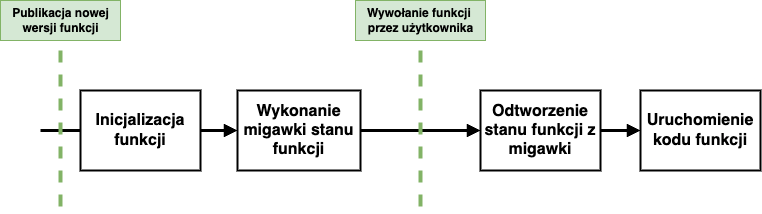
\includegraphics[width=0.95\textwidth]{charts/snapstart.png}
    \caption{Proces uruchomienia AWS Lambda z użyciem metody SnapStart [źródło:~opracowanie~własne]}
    \label{fig:aws_lambda_snapstart_process}
\end{figure}

Działanie tej metody jest technicznie możliwe dzięki użyciu środowiska wirtualizacji przez AWS Lambda.
Jak opisują Agache i inni autorzy \cite{246288} usługa Lambda do izolacji poszczególnych funkcji wykorzystuje dedykowane maszyny wirtualne typu microVM.
Są one zarządzane przez lekki monitor maszyn wirtualnych (ang. VMM) o nazwie Firecracker.
Posiada on cechy, które były kluczowe w minimalizacji problemu zimnego startu.
Po pierwsze, celowo rezygnuje on z emulacji zbędnych urządzeń (jak emulacja systemu BIOS czy rozbudowanych kontrolerów PCI) \cite{246288}.
Zmniejsza to złożoność i rozmiar stanu każdej maszyny wirtualnej. 
Dzięki temu wykonanie i odtworzenie migawki jest łatwiejsze.
Po drugie, Firecracker jest w pełni kontrolowany przez interfejs REST API \cite{246288}.
Umożliwia to precyzyjne zarządzanie całym cyklem życia każdej maszyny wirtualnej, włączając w to jej konfigurację, uruchomienie oraz zatrzymanie.
Pozwala to na określenie fazy inicjalizacji funkcji oraz wykonanie migawki w odpowiednim momencie.
Istotna jest również zapewniona przez Firecracker izolacja \cite{246288}, co gwarantuje bezpieczeństwo tworzenia i odtwarzania migawek.

Samo użycie metody SnapStart jest bardzo proste i nie wymaga od programisty dużego nakładu pracy.
Włączenie rozwiązania wymaga jedynie ustawienia odpowiedniej opcji podczas konfiguracji funkcji \cite{amazonSnapstartDeveloperGUide}.
Nie oznacza to jednak, że SnapStart jest odpowiedni dla wszystkich funkcji.
AWS podkreśla dwa typy aplikacji, które znacząco zyskają poprzez użycie SnapStart \cite{amazonSnapstartDeveloperGUide}.
Są nimi wrażliwe na opóźnienia interfejsy API i potoki przetwarzania danych.
Dodatkowo, metoda ta niesie za sobą pewne ograniczenia, które muszą zostać uwzględnione przed jej wdrożeniem.

Pierwszym aspektem jest kwestia unikalności stanu w funkcjach wykorzystujących SnapStart.
Jak analizują Brooker i inni autorzy \cite{brooker2021restoringuniquenessmicrovmsnapshots}, klonowanie migawek wprowadza fundamentalne wyzwanie związane z przywróceniem unikalności maszyn wirtualnych, co jest niezbędne do poprawnego generowania unikalnych identyfikatorów czy sekretów kryptograficznych.
Migawka zainicjowanego środowiska wykonywana jest jednorazowo, a następnie używana podczas wielu wywołań funkcji.
Może to stanowić duże zagrożenie dla programisty AWS Lambda, gdy potrzebuje on generować unikalne wartości jak identyfikatory (np. UUID) czy jednorazowe tokeny.
Narusza to znacznie poprawność logiki aplikacji oraz jej bezpieczeństwo.
Jedną z metod naprawy tego problemu jest generowanie wartości losowych wyłącznie w metodzie wywołującej funkcje (zamiast w bloku statycznym kodu) \cite{amazonSnapstartDeveloperGUide}.
Dodatkowo, ewentualne problemy z unikalnością funkcji SnapStart mogą zostać wykryte poprzez oprogramowanie SpotBugs \cite{SpotBugsProject}.
Narzędzie wykonuje statyczną analizę kodu, walidując go poprzez reguły zapewnione przez AWS.
Pozwala to programiście wykryć, a następnie naprawić fragmenty kodu powodujące problem z unikalnością.

Kolejnym istotnym wyzwaniem podczas rozwoju aplikacji z technologią SnapStart jest zarządzanie połączeniami sieciowymi \cite{amazonSnapstartDeveloperGUide}.
Połączenia nawiązane z zewnętrznymi usługami są standardową praktyką podczas tworzenia aplikacji AWS Lambda \cite{eismann2021reviewserverlessusecases}\cite{Ivanov_Petrova_2024}.
Problematyczne stają się jednak te połączenia sieciowe, które nawiązano podczas inicjalizacji funkcji. 
Ponieważ inicjalizacja odbywa się przed faktycznym przetworzeniem żądania użytkownika, upływający czas może sprawić, że w momencie odtworzenia funkcji połączenia te nie będą już aktywne.
Praktyką zalecaną przez AWS jest ponowne nawiązywanie lub dokładna walidacja istniejących połączeń \cite{amazonSnapstartDeveloperGUide}.
Powinno to być wykonane bezpośrednio w metodzie wywołującej funkcje lub z wykorzystaniem metody ,,afterRestore''.
Metoda ta jest wywoływana bezpośrednio po odtworzeniu migawki stanu funkcji.

Strategicznym czynnikiem usług bezserwerowych są koszty, zatem powinny być one uwzględnione także przed użyciem SnapStart.
Zgodnie z dokumentacją Amazon Web Services \cite{amazonSnapstartDeveloperGUide}, użycie SnapStart dla środowisk uruchomieniowych Java nie wiążą się z dodatkowymi kosztami.
Koszt wykonania funkcji z włączonym SnapStart nadal bazuje na standardowych rozliczeniach.
Składa się na niego liczba przetworzonych żądań oraz łączny czas trwania wykonań.

Podsumowując, mechanizm SnapStart stanowi prostą w aktywacji metodę redukcji czasu zimnych startów.
Sam mechanizm opiera się na wcześniejszym wykonaniu fazy inicjacji funkcji, a następnie wykonania migawki stanu.
W momencie wywołania funkcji stan ten może zostać odtworzony.
Znaczącą korzyścią metody jest brak dodatkowych kosztów.
Wiąże się ona jednak z istotnymi utrudnieniami (jak zarządzanie połączeniami sieciowymi i problem z unikalnością stanu).
Powinny być one uwzględnione przez programistę przed użyciem narzędzia.
\section{GraalVM}\label{chapter:graalvm}

Ważnym obszarem badań nad optymalizacją Javy i jej użycia w AWS Lambda, są technologie pozwalające na zmianę sposobu kompilacji i uruchamiana aplikacji.
Jedną z technologii, które zyskusje na popularności w tym zakresie, jest GraalVM.
Jest to możliwe m.in. dzięki użyciu kompilatora JIT (ang. Just-In-Time) w połączeniu z kompilacją AOT (ang. Ahead-Of-Time) \cite{8756917}.
GraalVM oferuje zaawansowaną architekturę pozwalającą na kompilację i uruchomienie aplikacji w postaci obrazów natywnych.
Stanowi to alternatywę dla klasycznej maszyny wirtualnej Javy, a dodatkowo skupia się na jej wydajności.
Poniższy podrozdział poświęcono analizie działania omawianego rozwiązania, jego zalet i słabych stron.

Kluczowym mechanizmem GraalVM jest kompilacja AOT (ang. Ahead-Of-Time) do postaci tzw. obrazów natywnych (ang. native images) \cite{8756917}.
Ma to bezpośredni wpływ na wydajność działania aplikacji.
W modelu tradycyjnym, kod bajtowy Java jest interpretowany i kompilowany dynamicznie przez maszynę wirtualną w trakcie działania aplikacji.
Podejście AOT przenosi znaczną część z tych operacji na etap budowania artefaktu. 
Istotnym elementem tego procesu jest agresywna, statyczna analiza kodu \cite{9245290}, w celu identyfikacji osiągalnych w trakcie działania części.
Pozwala to na odrzucenie nieużywanych fragmentów kodu (np. z używanych bibliotek), co pozwala na zmniejszenie wielkości obrazu natywnego.
Aspekt ten może być kluczowy w kontekście AWS Lambda, ze względu na wpływ wielkości artefaktu na wydajność \cite{8116416}.
Po analizie kodu, dokonywana jest inicjalizacja klas, a stan aplikacji, w tym częściowo zainicjalizowana sterta, jest utrwalany.
W celu lepszej optymalizacji, operacje te są powtarzane, co zostało przedstawione na Rysunku \ref{fig:graalvm_build_process}.

Jako wynik kompilacji powstaje samodzielny, zoptymalizowany plik binarny.
Nie wymaga on do uruchomienia pełnej maszyny wirtualnej Java, a jedynie minimalnego środowiska wykonawczego dostarczanego przez SubstrateVM, będącego częścią GraalVM \cite{8756917}.
Różnica ta ma fundamentalne znaczenie w kontekście wydajności AWS Lambda.
Eliminowana jest konieczność wykonywania czasochłonnych operacji typowych dla startu tradycyjnej maszyny wirtualnej Java, takich jak ładowanie klas czy jej inicjalizacja.
Wszystkie te zadania zostały już wykonane wcześniej, w procesie budowy obrazu natywnego.
Dzięki temu tworzona przez programistę funkcja AWS Lambda nie będzie operować w zarządzanym środowisku Java.
Zamiast tego, usługi muszą opierać się o niestandardowe środowiska wykonawcze, oferujące wyłącznie system operacyjny (Amazon Linux 2023 lub Amazon Linux 2) \cite{awsLambdaDeveloperGuide}.
Ich użycie pozwala także na realizację drugiej zalety GraalVM, czyli redukcji zapotrzebowania na pamięć operacyjną \cite{9245290}.

Pomimo pozytywnego wpływu na wydajność, zastosowanie kompilacji AOT w GraalVM wiąże się także z ograniczeniami.
Jednym z nich jest obsługa dynamicznych cech Javy, takich jak refleksja (ang. reflection), dynamiczne proxy, serializacja czy natywny interfejs Java (JNI)
Wynika to z faktu użycia agresywnej statycznej analizy kodu.
Napotyka ona trudności w przewidzeniu wszystkich dynamicznie ładowanych klas, pól i metod, które nie są jawnie osiągalne w kodzie źródłowym.
Problem ten wymaga użycia dodatkowych mechanizmów GraalVM \cite{graalvm-reflection-jdk21}.
Polegają one na przygotowaniu dodatkowych metadanych dla klas, co wymaga jednak dodatkowej obsługi.

\begin{figure}
    \centering
    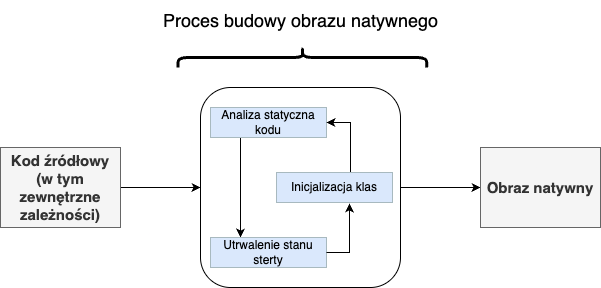
\includegraphics[width=0.95\textwidth]{charts/graalvm-build-process.drawio.png}
    \caption{Uproszczony proces budowy obrazu natywnego GraalVM [źródło:~opracowanie~własne]}
    \label{fig:graalvm_build_process}
\end{figure}

Kolejnym aspektem, który może negatywnie wpłynąć na rozwój oprogramowania przy użyciu GraalVM, jest czasochłonność procesu kompilacji.
Generowanie w pełni zoptymalizowanego obrazu natywnego jest operacją bardziej złożoną niż standardowa kompilacja kodu Javy do postaci bajtowej.
W praktyce oznacza to, że proces budowania artefaktu dla funkcji AWS Lambda może trwać odczuwalnie dłużej.
Może mieć to znaczący wpływ na rozwój oprogramowania, szczególnie w przypadku częstych iteracji i tworzenia nowych wersji funkcji.
Dłuższy czas kompilacji może także wpłynąć na ogólną efektywność procesów ciągłej integracji i ciągłego dostarczania (ang. CI/CD).

Jednym z sposobów poprawy doświadczeń programistów przy pracy z GraalVM, jest użycie odpowiednich frameworków.
Jednym z nich jest Quarkus \cite{9245290}, który został zaprojektowany z myślą o środowiskach chmurowych.
Kluczową cechą Quarkusa jest przeniesienie jak największej liczby operacji inicjalizacyjnych i konfiguracyjnych na etap budowania aplikacji.
Obejmuje to między innymi wstrzykiwanie zależności, przetwarzanie adnotacji oraz konfigurację rozszerzeń. 
Dzięki temu, w czasie budowania obrazu natywnego, Quarkus jest w stanie przeprowadzić szczegółową analizę aplikacji.
Poprzez użycie odpowiednich annotacji pozwala on na oznaczenie klas niezbędnych dla mechanizmów refleksji czy proxy \cite{quarkus-docs}.
Dzięki temu jest on w stanie automatycznie wygenerować niezbędne metadane dla klas.
Dane te następnie pozwalają na użycie wspomnianych mechanizmów w GraalVM.
Innymi, konkurencyjnymi do Quarkusa frameworkami, które oferują wsparcie dla obrazów natywnych są Helidon i Micronaut \cite{9245290}.
Ich popularność wskazuje na wysokie zainteresowanie takimi technologiami w społeczności programistów Java, dlatego jest to interesujący kierunek rozwoju dla funkcji AWS Lambda.

\section{Kotlin}\label{chapter:kotlin_multiplatform}

W ramach systematycznego przeglądu literatury (przedstawionego w Rozdziale \ref{chapter:przeglad_literatury}) zauważono, że aktualne badania skupiają się wyłącznie na języku Java.
Pomijają one jednak inne języki z ekosystemu Java, także oparte o maszynę wirtualną Java (ang. JVM).
Tymczasem na popularności zyskują alternatywne języki ekosystemu Javy.
Wśród nich na szczególną uwagę zasługuje Kotlin, rozwijany przez firmę JetBrains.
Jest on oficjalnie wspierany przez Google jako język programowania dla platformy Android, co wskazuje na jego solidne zastosowanie w tych systemach.
Coraz większe uznanie zyskuje także jako działający po stronie serwera. 
Dlatego język ten jest interesującym obszarem badań w kontekście AWS Lambda.
W tym rozdziale przedstawiony zostanie język programowania Kotlin, w tym jego zastosowanie w kontekście funkcji AWS Lambda.

Jednym z kluczowych czynników, które zwiększają popularność Kotlina, jest jego łatwa nauka przez programistów Javy.
Dodatkowo, istnieje możliwość łatwej intergracji kodu napisanego w Kotlinie z istniejącym oprogramowaniem Java \cite{kotlinlangKotlinDocs}.
Te cechy czynią go interesującym kandydatem do analizy w kontekście optymalizacji wydajności rozwiązań dla usługi AWS Lambda. 
Dla zespołów programistycznych może stanowić on wartościowe rozszerzenie dotychczasowych możliwości. 
Kotlin oferuje bowiem alternatywę lub uzupełnienie dla tradycyjnie stosowanej Javy.

Kwestia wydajności Kotlina w porównaniu do Javy jest przedmiotem dyskusji. 
Jednak badania dotyczą najczęściej ich zastosowań w kontekście aplikacji mobilnych.
Gajek i inni autorzy \cite{Gajek_Plechawska-Wójcik_2024} przeanalizowali wydajność obu języków, poprzez użycie gry mobilnej uruchomionej na systemie Android.
Wykazali oni, że w testowanym scenariuszu Java osiągnęła nieznacznie lepszą wydajność pod względem zużycia zasobów CPU i RAM.
Było to jednak zastosowanie mobilne, a same różnice nie były znaczne.
Należy jednak podkreślić, że warunki mobilne mogą być inne niż w systemach działających w usłudze AWS Lambda.
Sam język Kotlin posiada mechanizmy, które mogą pozytywnie wpłynąć na wydajność.

Funkcje inline (ang. inline functions) w Kotlinie mogą przyczynić się do redukcji narzutu wydajności podczas wywołań funkcji.
Mechanizm ten polega na wstawieniu kodu ciała funkcji bezpośrednio w miejsce jej wywołania \cite{kotlinlangKotlinDocs}.
Jest to wykonywane w momencie kompilacji, a programista może określić, które funkcje powinny być w ten sposób optymalizowane.
Eliminuje to koszt ich wywołania, co jest szczególnie przydatne w przypadku małych, często używanych funkcji.
Dodatkowo, język pozwala na przekazywanie funkcji jako parametrów, na przykład w kolekcjach i metodach jak filtrowanie.
W tych sytuacjach użycie funkcji inline może znacząco zmniejszyć liczbę operacji.
Pozytywny wpływ mechanizmu inline został przedstawiony przez Bergstrom i innych autorów \cite{DBLP:journals/corr/BergstromFRS13}, gdzie jego użycie zmniejszyło czas wykonywania programów nawet do 8\%.

Innym istotnym elementem Kotlina wspierającym wydajność są korutyny (ang. coroutines).
Mogą być one użyteczne zwłaszcza w kontekście operacji wejścia-wyjścia (I/O).
Systemy oparte o usługę AWS Lambda często integrowane są z zewnętrznymi serwisami (co zostało zauważone w ramach przeglądu literatury w Rozdziale \ref{chapter:przeglad_literatury}).
Wymaga to komunikacji opartej o operacje sieciowe.
Tradycyjne podejście oparte na wątkach może konsumować dużą ilość zasobów serwera i prowadzić do blokowania wykonania.
Korutyny pozwalają na pisanie asynchronicznego, nieblokującego kodu w sposób bardziej sekwencyjny i czytelny \cite{kotlinlangKotlinDocs}.
Na lepszą wydajność korutyn w porównaniu z tradycyjnymi wątkami wskazali Beronić i inni autorzy \cite{9803765}.

Implementacja mechanizmów poprawiających wydajność w języku programowania, pozwala następnie na ich użycie w bibliotekach, które są wykorzystywane przez programistów.
Język Kotlin oferuje ciekawy ekosystem bibliotek, przeznaczonych na przykład do tworzenia aplikacji działających po stronie serwera.
Są to biblioteki jak http4k czy ktor.
Ktor to framework zaprojektowany do budowy asynchronicznych aplikacji serwerowych i klienckich, rozwijany przez firmę JetBrains.
Jest on oparty w pełni o język Kotlin, a jego kluczową cechą jest natywne wsparcie dla korutyn.
Z kolei http4k kładzie nacisk na prostotę i minimalizm.
Architektura http4k opiera się na koncepcji funkcji jako podstawowych bloków aplikacji \cite{http4kCoreDocs}, co naturalnie współgra z modelem serverless i AWS Lambda.
Samo narzędzie rezyguje z mechanizmów refleksji \cite{http4kCoreDocs}, co może mieć pozytywny wpływ na wydajność.

Rosnące znaczenie Kotlin dostrzega także Amazon Web Service, które oferuje bibliotekę AWS SDK dla Kotlina \cite{awsSDKForKotlinDeveloperGuide}.
Jej celem jest zapewnienie programistom możliwości interakcji z usługami AWS w sposób naturalny dla tego języka.
SDK ten został zaprojektowany od podstaw z myślą o Kotlinie, co przejawia się między innymi w wykorzystaniu korutyn do obsługi operacji asynchronicznych.

Duży wpływ na wydajność funkcji AWS Lambda ma wybrany język programowania \cite{8605773}\cite{Cordingly2020704}.
Wynika to na przykład z różnych przypadków biznesowych i operacji, które muszą wykonywać.
Mimo to, często muszą one dzielić wspólny kod \cite{8116416}, co wskazuje na potrzebę wykorzystania mechanizmów, które to umożliwą.
Z tego powodu bardzo interesującą dla AWS Lambda i jej wydajności, może okazać się inicjatywa Kotlin Multiplatform.
KMP (Kotlin Multiplatform) to projekt, który powstał w szczególności dla aplikacji mobilnych.
Pozwala on na kompilację lub translację tego samego kodu Kotlin do użycia na różnych platformach.
Mogą to być na przykład Android, iOS, aplikacje desktopowe (JVM) lub webowe (JavaScript, Web Assembly) \cite{kotlinlangKotlinDocs}.
Oferuje to możliwość dzielenia kodu (np. logiki biznesowej) pomiędzy różnymi platformami, jednak przy możliwości zachowania natywnych komponentów widoku.

Mimo głównego przypadku użycia jakim są aplikacje klienckie, Kotlin Multiplatform może być obiecującym rozwiązaniem dla AWS Lambda.
Po pierwsze oferuje on możliwość translacji kodu Kotlin do JavaScript oraz kompilację do natywnych plików binarnych (opcje te zostaną przedstawione jako osobne metody w kolejnych rozdziałach).
Pozwala to na ominięcie różnych niedogodności wynikających z użycia maszyny wirtualnej Javy.
Jednak zachowane są przy tym zalety języka oraz wspiera to użycie już istniejących umiejętności programistów języków rodziny JVM.
Po drugie, kod w KMP może być dzielony pomiędzy platformami.
Umożliwia to bardzo elastyczny wybór środowiska uruchomieniowego AWS Lambda w ramach pojedynczego systemu.
Jednocześnie, część kodu może być współdzielona między wszystkie funkcje niezależnie od wybranej platformy.
Może to na przykład oznaczać, że klasy implementujące pewne struktury oraz zasady wynikające z reguł biznesowych, będą mogły być używane przez funkcje działające zarówno poprzez JavaScript, JVM, jak i natywne pliki binarne. 

Jednym z czynników, które mogą być modyfikowane już podczas działania usług AWS Lambda jest pamięć.
Jej rozmiar może być dostosowywany w zależności od wydajności monitorowanej funkcji.
Użycie Kotlin Multiplatform pozwala na rozszerzenie tej metody.
W zależności od obserwowanych parametrów (jak czas odpowiedzi lub opóźnienia zimnych startów) możliwe jest ponowne wykorzystanie tego samego kodu i budowa funkcji działającej na innej platformie.
Przykładowo, po wdrożeniu funkcji działającej z użyciem JVM, może pojawić się potrzeba redukcji czasu zimnych startów.
W takim wypadku Kotlin Multiplatform umożliwia translację kodu do JavaScript, który pozwoli na redukcję czasu inicjalizacji AWS Lambda.

Współdzielenie kodu pomiędzy platformami jest możliwe dzięki strukturze, którą oferuje Kotlin Multiplatform.
Została ona opisana przez firmę JetBrains w ramach dokumentacji KMP \cite{kotlinMultiplatformDev}.
Jej głównym elementem jest katalog ,,commonMain'', który jest współdzielony pomiędzy wszystkimi platformami.
Kompilator używa kodu współdzielonego jako dane wejściowe, aby w rezultacie utworzyć zestaw plików binarnych specyficznych dla danej platformy.
Mogą to być na przykład pliki .class dla maszyny wirtualnej Javy, czy natywne pliki wykonywalne (np. dla platformy Linux).

\begin{figure}[h]
    \centering
    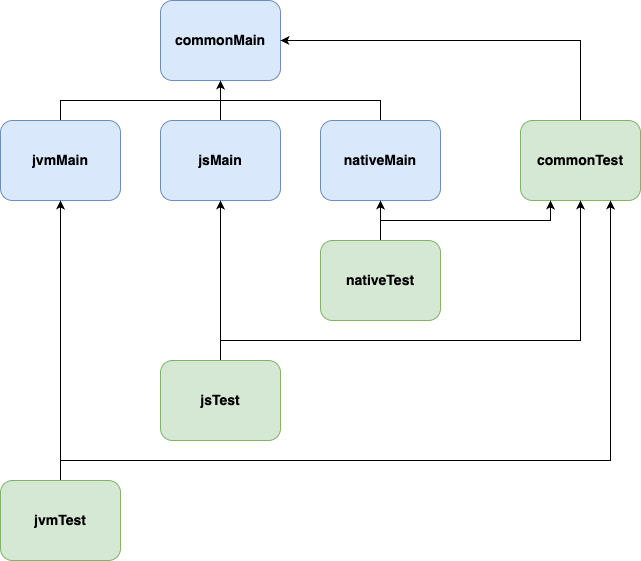
\includegraphics[width=0.95\textwidth]{charts/kmp-structure.drawio.png}
    \caption{Przykładowa struktura pojektu Kotlin Multiplatform [źródło:~opracowanie~własne]}
    \label{fig:kmp_project_structure}
\end{figure}

Następnie programista może utworzyć kolejne katalogi, które będą zawierać kod specyficzny dla docelowych platform.
Przykładowa struktura została przedstawiona na Rysunku \ref{fig:kmp_project_structure}, gdzie katalog commonMain jest wspóldzielony między JVM (jvmMain), JavaScript (jsMain) oraz platformy natywne (nativeMain).
Docelowe platformy (ang. targets) są deklarowane w konfiguracji Gradle \cite{kotlinMultiplatformDev}, a kod współdzielony jest przygotowywany wyłącznie dla nich.
Katalogi dla docelowych platform są wymagane, gdyż Kotlin nie zezwala na użycie specyficznych elementów danej platformy w katalogu współdzielonym.
Przykładem takiego elementu może być klasa ,,java.io.File'', która jest dostępna wyłącznie dla maszyny wirtualnej Javy.
Jej użycie w katalogu commonMain spowoduje błąd kompilacji.

Kotlin Multiplatform zawiera także integracje z testami oprogramowania.
Jest to szczególnie ważne dla tworzenia oprogramowania z wykorzystaniem AWS Lambda, gdzie testowanie może być skomplikowane (co było jednym z wniosków przeglądu literatury w Rozdziale \ref{chapter:przeglad_literatury}).
Testy dla kodu współdzielonego powinny być zapisane w katalogu ,,commonTest'', gdzie programista może użyć biblioteki kotlin.test \cite{kotlinMultiplatformDev}.
Następnie testy są uruchamiane dla każdej docelowej platformy.
Programista może także tworzyć przypadki testowe dla konkretnych platform, z użyciem technologii przez nie oferowanych.
Następuje tutaj analogiczne współdzielenie kodu jak dla katalogów ,,main'', co zostało także zawarte w Rysunku \ref{fig:kmp_project_structure}.

Specyficzne cechy Kotlina jak funkcjonalności języka, biblioteki czy projekt Kotlin Multiplatform mogą zapewnić znaczne wzrosty wydajności funkcji AWS Lambda.
Mimo, że Kotlin jest językiem wywodzącym się z Javy oferuje już możliwości, które mogą pozwolić na osiągnięcie niższych czasów odpowiedzi.
Dodatkowo, sposoby te nie zostały jeszcze przebadane. 
Dlatego Kotlin to obszar, który zasługuje na zawarcie go w badanich na temat wydajności AWS Lambda.

\section{Kotlin/JS}\label{chapter:kotlin_js}

\section{Kotlin/Native}\label{chapter:kotlin_native}

Bardzo skuteczną metodą optymalizacji wydajności może być rezygnacja z zarządzanych środowisk uruchomieniowych jak JVM.
Jedną z metod jest kompilacja do kodu natywnego, który uruchamiany jest bezpośrednio na systemie operacyjnym poza maszyną wirtualną.
Kotlin/Native oferuje zaawansową kompilację kodu Kotlin, który następnie może zostać uruchomiony w AWS Lambda z użyciem Amazon Linux.
W ramach rozdziału opisano sposób działania Kotlin/Native, jego możliwości i cechy, które mogą negatywnie wpłynąć na rozwój oprogramowania bezserwerowego.

Kluczowym elementami Kotlin/Native są kompilator oparty o LLVM oraz natywne implementacje bibliotek standardowych Kotlina \cite{kotlinlangKotlinDocs}.
Jak opisują Lattner i Adve \cite{1281665}, LLVM to framework kompilatora zaprojektowany do wspierania ciągłej i transparentnej analizy oraz transformacji programów.
Definiuje on wspólną, niskopoziomową reprezentację kodu w formie SSA (ang. Static Single Assignment) z systemem typów niezależnym od języka, co umożliwia implementację cech języków wysokiego poziomu. 
Głównym celem LLVM jest umożliwienie analizy i transformacji programu na różnych etapach jego życia, w tym w czasie kompilacji, linkowania, uruchomienia oraz w czasie bezczynności między uruchomieniami.
Jego użycie pozwala następnie na zbudowanie natywnych plików binarnych, które mogą zostać uruchomione bezpośrednio na docelowej platformie, dla której zostały skompilowane.
Wymaga to jednak dokładnego określenia systemu operacyjnego i architektury już w momencie kompilacji.

Kompilacja Kotlina do kodu natywnego otwiera przez KMP możliwość tworzenia samodzielnych programów wykonywalnych, które nie wymagają zewnętrznego środowiska uruchomieniowego.
Znajduje to zastosowanie w scenariuszach takich jak rozwój aplikacji mobilnych na platformę iOS, współdzielenie logiki biznesowej między różnymi platformami (np. Android i iOS) czy budowa narzędzi konsolowych.
Dlatego ważnym aspektem Kotlin/Native jest współdziałanie z istniejącym kodem natywnym.
Pozwala to na bezpośrednie wywoływanie funkcji z bibliotek napisanych w języku C, a na platformach firmy Apple również Objective-C \cite{kotlinlangKotlinDocs}.
Znacząco rozszerza to zakres dostępnych narzędzi i bibliotek, które mogą zostać użyte przez programistów.

Kotlin/Native oferuje wiele różnych platform docelowych, rozszerzając tym samym zakres zastosowań języka Kotlin.
Wśród wspieranych systemów docelowych znajdują się platformy Apple (takie jak macOS, iOS, watchOS, tvOS), Android, a także systemy z rodziny Windows oraz Linux \cite{kotlinlangKotlinDocs}.
Szczególnie istotnie dla usługi AWS Lambda są jednak platformy linuxowe.
Są to linuxX64 oraz linuxArm64, które pozwalają na uruchomienie kodu z użyciem odpowiednio architektur x86 oraz ARM.
Pozwala to następnie na ich bezpośrednie użycie w AWS Lambda, działającej bezpośrednio w systemie Amazon Linux.
Dzięki temu możliwa jest poprawa wydajności, szczególnie w aspekcie zimnych startów, które są znacznym wyzwaniem dla funkcji opartych o JVM.

Istotnym elementen funkcji bezserwerowych jest zarządzanie pamięcią, która wpływa bezpośrednio na koszty.
W przypadku Kotlin/Native, ewolucja modelu zarządzania pamięcią znacząco wpłynęła na jego użyteczność i możliwości optymalizacyjne.
Początkowa technologia ta opierała się na restrykcyjnym modelu z izolacją obiektów między wątkami \cite{kotlinlangKotlinDocs}.
Powodowało to skomplikowane zarządzanie stanem w operacjach współbieżnych.
Aktualnie, Kotlin/Native implementuje nowy menedżer pamięci.
Wprowadza on automatyczne zarządzanie pamięcią poprzez współbieżny, nieblokujący moduł zbierania śmieci (ang. garbage collector) \cite{kotlinlangKotlinDocs}.
Znacząco upraszcza to programowanie współbieżne, które teraz nie wymaga ręcznego zarządzania obiektami.
Mechanizm ten wprowadza intuicyjne współdzielenie stanu, które jest analogiczne do środowiska JVM, jednak bez konieczności kosztownej obsługi maszyny wirtualnej Java.

Mimo potencjalnych zysków w ramach wydajności, użycie Kotlin/Native może nieść utrudnienia w kontekście integracji z bibliotekami zewnętrznymi.
Język C nie jest oficjalnie wspierany jako język programowania AWS Lambda \cite{awsLambdaDeveloperGuide}, co wynika zapewne z jego niewielkiej popularności na tej platformie.
Współdziałanie z kodem natywnym w Kotlin/Native skupia się jednak na platformach klienckich, co nie musi być do końca użyteczne w zakresie AWS Lambda.
Amazon Web Services oferuje swoje SDK w języku C++, który nie jest jednak łatwo integrowalny z Kotlin/Native (w odróżnieniu od C i Objective-C).
Jest to ważny czynnik, który powinien być uwzględniony przez programistów projektujących aplikacje bezserwerowe.

% Plan
% 0. Wstęp

% 1. Jak to działa:
% - Opisać LLVM
% - Gdzie się głównie używa
% - Wspomnieć o interoperacyjności z C, Objective-C itp
% - Jakie platformy? (https://kotlinlang.org/docs/native-target-support.html#for-library-authors)

% 2. Zarządzanie pamięcią (https://kotlinlang.org/docs/native-memory-manager.html)

% 3. Wady - problem z dostępnością bibliotek
% - AWS SDK może poprzez C++ jednak może to wymagać większego nakładu pracy


\chapter*{Słownik pojęć}
\addcontentsline{toc}{chapter}{Słownik pojęć i akronimów}  

Ekosystem Java

Serverless

AWS

FaaS

BaaS

Zimny start

Ciepły start

JVM



\newpage
\pagestyle{custom}
\chapter{Wybrane metody optymalizacji}\label{chapter:wybrane_metody_optimalizacji}

% TODO: jakiś wstęp, typu jakich metod brakowało w przeglądzie. Podkreślić brak innych języków
\section{SnapStart}\label{chapter:snapstart}

Jednym z istotnych czynników wpływających na wydajność funkcji AWS Lambda implementowanych w ekosystemie Java jest zjawisko tzw. zimnego startu.
Wynika on z cyklu życia funkcji i etapu inicjalizacji (co zostało opisane w Rozdziale \ref{chapter:aws_lambda}).
W etap ten wchodzą procesy takie jak inicjalizacja maszyny wirtualnej Java czy uruchomienie statycznego kodu inicjującego \cite{awsLambdaDocs}.
W przypadku Javy zajmuje to więcej czasu niż dla innych języków (jak Python), co wydłuża zimne starty \cite{8605773}.
Znacząco oddziałuje to na wydajność funkcji, a może być szczególnie dotkliwe dla serwisów o niewielkiej aktywności.
W odpowiedzi na potrzebę minimalizacji tych negatywnych skutków Amazon Web Services wprowadziło mechanizm znany jako AWS Lambda SnapStart.
W ramach podrozdziału podjęto analizę tego rozwiązania w kontekście jego działania, zalet oraz ograniczeń. 

Mechanizm SnapStart istotnie modyfikuje tradycyjny cykl życia funkcji AWS Lambda.
Zasadnicza różnica polega na przeniesieniu kosztownego etapu inicjalizacji z momentu pierwszego wywołania funkcji na etap jej publikacji \cite{amazonSnapstartDeveloperGUide}.
Oznacza to, że inicjalizacja funkcji nie jest wykonywana w momencie zapytania użytkownika (co wywołuje zimny start), lecz w momencie wgrania nowej wersji funkcji (oraz kodu) przez programistę.
Inicjalizacja ta zawiera najdłuższe operacje dla rozwiązań Java jak utworzenie maszyny wirtualnej, załadowanie klas, czy wykonanie kodu inicjalizującego.
Następnie, tworzona jest zaszyfrowana ,,migawka'' (ang. snapshot) stanu pamięci i dysku w pełni gotowego środowiska wykonawczego.
Gdy funkcja jest następnie wywoływana po raz pierwszy, nie zachodzi już standardowy zimny start.
Zamiast tego środowisko jest odtwarzane z utworzonej migawki, co zostało przedstawione na Rysunku \ref{fig:aws_lambda_snapstart_process}.
Według dostawcy AWS metoda ta w optymalnych scenariuszach zmniejsza opóźnienie z kilku sekund do mniej niż sekundy \cite{amazonSnapstartDeveloperGUide}. 

\begin{figure}[h]
    \centering
    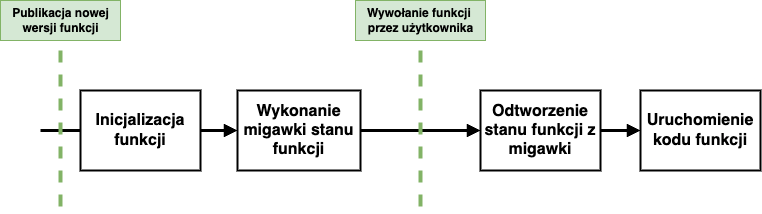
\includegraphics[width=0.95\textwidth]{charts/snapstart.png}
    \caption{Proces uruchomienia AWS Lambda z użyciem metody SnapStart [źródło:~opracowanie~własne]}
    \label{fig:aws_lambda_snapstart_process}
\end{figure}

Działanie tej metody jest technicznie możliwe dzięki użyciu środowiska wirtualizacji przez AWS Lambda.
Jak opisują Agache i inni autorzy \cite{246288} usługa Lambda do izolacji poszczególnych funkcji wykorzystuje dedykowane maszyny wirtualne typu microVM.
Są one zarządzane przez lekki monitor maszyn wirtualnych (ang. VMM) o nazwie Firecracker.
Posiada on cechy, które były kluczowe w minimalizacji problemu zimnego startu.
Po pierwsze, celowo rezygnuje on z emulacji zbędnych urządzeń (jak emulacja systemu BIOS czy rozbudowanych kontrolerów PCI) \cite{246288}.
Zmniejsza to złożoność i rozmiar stanu każdej maszyny wirtualnej. 
Dzięki temu wykonanie i odtworzenie migawki jest łatwiejsze.
Po drugie, Firecracker jest w pełni kontrolowany przez interfejs REST API \cite{246288}.
Umożliwia to precyzyjne zarządzanie całym cyklem życia każdej maszyny wirtualnej, włączając w to jej konfigurację, uruchomienie oraz zatrzymanie.
Pozwala to na określenie fazy inicjalizacji funkcji oraz wykonanie migawki w odpowiednim momencie.
Istotna jest również zapewniona przez Firecracker izolacja \cite{246288}, co gwarantuje bezpieczeństwo tworzenia i odtwarzania migawek.

Samo użycie metody SnapStart jest bardzo proste i nie wymaga od programisty dużego nakładu pracy.
Włączenie rozwiązania wymaga jedynie ustawienia odpowiedniej opcji podczas konfiguracji funkcji \cite{amazonSnapstartDeveloperGUide}.
Nie oznacza to jednak, że SnapStart jest odpowiedni dla wszystkich funkcji.
AWS podkreśla dwa typy aplikacji, które znacząco zyskają poprzez użycie SnapStart \cite{amazonSnapstartDeveloperGUide}.
Są nimi wrażliwe na opóźnienia interfejsy API i potoki przetwarzania danych.
Dodatkowo, metoda ta niesie za sobą pewne ograniczenia, które muszą zostać uwzględnione przed jej wdrożeniem.

Pierwszym aspektem jest kwestia unikalności stanu w funkcjach wykorzystujących SnapStart.
Jak analizują Brooker i inni autorzy \cite{brooker2021restoringuniquenessmicrovmsnapshots}, klonowanie migawek wprowadza fundamentalne wyzwanie związane z przywróceniem unikalności maszyn wirtualnych, co jest niezbędne do poprawnego generowania unikalnych identyfikatorów czy sekretów kryptograficznych.
Migawka zainicjowanego środowiska wykonywana jest jednorazowo, a następnie używana podczas wielu wywołań funkcji.
Może to stanowić duże zagrożenie dla programisty AWS Lambda, gdy potrzebuje on generować unikalne wartości jak identyfikatory (np. UUID) czy jednorazowe tokeny.
Narusza to znacznie poprawność logiki aplikacji oraz jej bezpieczeństwo.
Jedną z metod naprawy tego problemu jest generowanie wartości losowych wyłącznie w metodzie wywołującej funkcje (zamiast w bloku statycznym kodu) \cite{amazonSnapstartDeveloperGUide}.
Dodatkowo, ewentualne problemy z unikalnością funkcji SnapStart mogą zostać wykryte poprzez oprogramowanie SpotBugs \cite{SpotBugsProject}.
Narzędzie wykonuje statyczną analizę kodu, walidując go poprzez reguły zapewnione przez AWS.
Pozwala to programiście wykryć, a następnie naprawić fragmenty kodu powodujące problem z unikalnością.

Kolejnym istotnym wyzwaniem podczas rozwoju aplikacji z technologią SnapStart jest zarządzanie połączeniami sieciowymi \cite{amazonSnapstartDeveloperGUide}.
Połączenia nawiązane z zewnętrznymi usługami są standardową praktyką podczas tworzenia aplikacji AWS Lambda \cite{eismann2021reviewserverlessusecases}\cite{Ivanov_Petrova_2024}.
Problematyczne stają się jednak te połączenia sieciowe, które nawiązano podczas inicjalizacji funkcji. 
Ponieważ inicjalizacja odbywa się przed faktycznym przetworzeniem żądania użytkownika, upływający czas może sprawić, że w momencie odtworzenia funkcji połączenia te nie będą już aktywne.
Praktyką zalecaną przez AWS jest ponowne nawiązywanie lub dokładna walidacja istniejących połączeń \cite{amazonSnapstartDeveloperGUide}.
Powinno to być wykonane bezpośrednio w metodzie wywołującej funkcje lub z wykorzystaniem metody ,,afterRestore''.
Metoda ta jest wywoływana bezpośrednio po odtworzeniu migawki stanu funkcji.

Strategicznym czynnikiem usług bezserwerowych są koszty, zatem powinny być one uwzględnione także przed użyciem SnapStart.
Zgodnie z dokumentacją Amazon Web Services \cite{amazonSnapstartDeveloperGUide}, użycie SnapStart dla środowisk uruchomieniowych Java nie wiążą się z dodatkowymi kosztami.
Koszt wykonania funkcji z włączonym SnapStart nadal bazuje na standardowych rozliczeniach.
Składa się na niego liczba przetworzonych żądań oraz łączny czas trwania wykonań.

Podsumowując, mechanizm SnapStart stanowi prostą w aktywacji metodę redukcji czasu zimnych startów.
Sam mechanizm opiera się na wcześniejszym wykonaniu fazy inicjacji funkcji, a następnie wykonania migawki stanu.
W momencie wywołania funkcji stan ten może zostać odtworzony.
Znaczącą korzyścią metody jest brak dodatkowych kosztów.
Wiąże się ona jednak z istotnymi utrudnieniami (jak zarządzanie połączeniami sieciowymi i problem z unikalnością stanu).
Powinny być one uwzględnione przez programistę przed użyciem narzędzia.
\section{GraalVM}\label{chapter:graalvm}

Ważnym obszarem badań nad optymalizacją Javy i jej użycia w AWS Lambda, są technologie pozwalające na zmianę sposobu kompilacji i uruchamiana aplikacji.
Jedną z technologii, które zyskusje na popularności w tym zakresie, jest GraalVM.
Jest to możliwe m.in. dzięki użyciu kompilatora JIT (ang. Just-In-Time) w połączeniu z kompilacją AOT (ang. Ahead-Of-Time) \cite{8756917}.
GraalVM oferuje zaawansowaną architekturę pozwalającą na kompilację i uruchomienie aplikacji w postaci obrazów natywnych.
Stanowi to alternatywę dla klasycznej maszyny wirtualnej Javy, a dodatkowo skupia się na jej wydajności.
Poniższy podrozdział poświęcono analizie działania omawianego rozwiązania, jego zalet i słabych stron.

Kluczowym mechanizmem GraalVM jest kompilacja AOT (ang. Ahead-Of-Time) do postaci tzw. obrazów natywnych (ang. native images) \cite{8756917}.
Ma to bezpośredni wpływ na wydajność działania aplikacji.
W modelu tradycyjnym, kod bajtowy Java jest interpretowany i kompilowany dynamicznie przez maszynę wirtualną w trakcie działania aplikacji.
Podejście AOT przenosi znaczną część z tych operacji na etap budowania artefaktu. 
Istotnym elementem tego procesu jest agresywna, statyczna analiza kodu \cite{9245290}, w celu identyfikacji osiągalnych w trakcie działania części.
Pozwala to na odrzucenie nieużywanych fragmentów kodu (np. z używanych bibliotek), co pozwala na zmniejszenie wielkości obrazu natywnego.
Aspekt ten może być kluczowy w kontekście AWS Lambda, ze względu na wpływ wielkości artefaktu na wydajność \cite{8116416}.
Po analizie kodu, dokonywana jest inicjalizacja klas, a stan aplikacji, w tym częściowo zainicjalizowana sterta, jest utrwalany.
W celu lepszej optymalizacji, operacje te są powtarzane, co zostało przedstawione na Rysunku \ref{fig:graalvm_build_process}.

Jako wynik kompilacji powstaje samodzielny, zoptymalizowany plik binarny.
Nie wymaga on do uruchomienia pełnej maszyny wirtualnej Java, a jedynie minimalnego środowiska wykonawczego dostarczanego przez SubstrateVM, będącego częścią GraalVM \cite{8756917}.
Różnica ta ma fundamentalne znaczenie w kontekście wydajności AWS Lambda.
Eliminowana jest konieczność wykonywania czasochłonnych operacji typowych dla startu tradycyjnej maszyny wirtualnej Java, takich jak ładowanie klas czy jej inicjalizacja.
Wszystkie te zadania zostały już wykonane wcześniej, w procesie budowy obrazu natywnego.
Dzięki temu tworzona przez programistę funkcja AWS Lambda nie będzie operować w zarządzanym środowisku Java.
Zamiast tego, usługi muszą opierać się o niestandardowe środowiska wykonawcze, oferujące wyłącznie system operacyjny (Amazon Linux 2023 lub Amazon Linux 2) \cite{awsLambdaDeveloperGuide}.
Ich użycie pozwala także na realizację drugiej zalety GraalVM, czyli redukcji zapotrzebowania na pamięć operacyjną \cite{9245290}.

Pomimo pozytywnego wpływu na wydajność, zastosowanie kompilacji AOT w GraalVM wiąże się także z ograniczeniami.
Jednym z nich jest obsługa dynamicznych cech Javy, takich jak refleksja (ang. reflection), dynamiczne proxy, serializacja czy natywny interfejs Java (JNI)
Wynika to z faktu użycia agresywnej statycznej analizy kodu.
Napotyka ona trudności w przewidzeniu wszystkich dynamicznie ładowanych klas, pól i metod, które nie są jawnie osiągalne w kodzie źródłowym.
Problem ten wymaga użycia dodatkowych mechanizmów GraalVM \cite{graalvm-reflection-jdk21}.
Polegają one na przygotowaniu dodatkowych metadanych dla klas, co wymaga jednak dodatkowej obsługi.

\begin{figure}
    \centering
    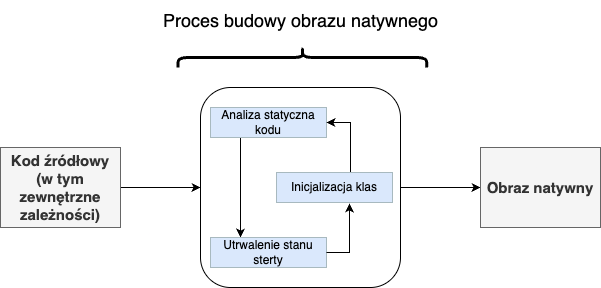
\includegraphics[width=0.95\textwidth]{charts/graalvm-build-process.drawio.png}
    \caption{Uproszczony proces budowy obrazu natywnego GraalVM [źródło:~opracowanie~własne]}
    \label{fig:graalvm_build_process}
\end{figure}

Kolejnym aspektem, który może negatywnie wpłynąć na rozwój oprogramowania przy użyciu GraalVM, jest czasochłonność procesu kompilacji.
Generowanie w pełni zoptymalizowanego obrazu natywnego jest operacją bardziej złożoną niż standardowa kompilacja kodu Javy do postaci bajtowej.
W praktyce oznacza to, że proces budowania artefaktu dla funkcji AWS Lambda może trwać odczuwalnie dłużej.
Może mieć to znaczący wpływ na rozwój oprogramowania, szczególnie w przypadku częstych iteracji i tworzenia nowych wersji funkcji.
Dłuższy czas kompilacji może także wpłynąć na ogólną efektywność procesów ciągłej integracji i ciągłego dostarczania (ang. CI/CD).

Jednym z sposobów poprawy doświadczeń programistów przy pracy z GraalVM, jest użycie odpowiednich frameworków.
Jednym z nich jest Quarkus \cite{9245290}, który został zaprojektowany z myślą o środowiskach chmurowych.
Kluczową cechą Quarkusa jest przeniesienie jak największej liczby operacji inicjalizacyjnych i konfiguracyjnych na etap budowania aplikacji.
Obejmuje to między innymi wstrzykiwanie zależności, przetwarzanie adnotacji oraz konfigurację rozszerzeń. 
Dzięki temu, w czasie budowania obrazu natywnego, Quarkus jest w stanie przeprowadzić szczegółową analizę aplikacji.
Poprzez użycie odpowiednich annotacji pozwala on na oznaczenie klas niezbędnych dla mechanizmów refleksji czy proxy \cite{quarkus-docs}.
Dzięki temu jest on w stanie automatycznie wygenerować niezbędne metadane dla klas.
Dane te następnie pozwalają na użycie wspomnianych mechanizmów w GraalVM.
Innymi, konkurencyjnymi do Quarkusa frameworkami, które oferują wsparcie dla obrazów natywnych są Helidon i Micronaut \cite{9245290}.
Ich popularność wskazuje na wysokie zainteresowanie takimi technologiami w społeczności programistów Java, dlatego jest to interesujący kierunek rozwoju dla funkcji AWS Lambda.

\section{Kotlin}\label{chapter:kotlin_multiplatform}

W ramach systematycznego przeglądu literatury (przedstawionego w Rozdziale \ref{chapter:przeglad_literatury}) zauważono, że aktualne badania skupiają się wyłącznie na języku Java.
Pomijają one jednak inne języki z ekosystemu Java, także oparte o maszynę wirtualną Java (ang. JVM).
Tymczasem na popularności zyskują alternatywne języki ekosystemu Javy.
Wśród nich na szczególną uwagę zasługuje Kotlin, rozwijany przez firmę JetBrains.
Jest on oficjalnie wspierany przez Google jako język programowania dla platformy Android, co wskazuje na jego solidne zastosowanie w tych systemach.
Coraz większe uznanie zyskuje także jako działający po stronie serwera. 
Dlatego język ten jest interesującym obszarem badań w kontekście AWS Lambda.
W tym rozdziale przedstawiony zostanie język programowania Kotlin, w tym jego zastosowanie w kontekście funkcji AWS Lambda.

Jednym z kluczowych czynników, które zwiększają popularność Kotlina, jest jego łatwa nauka przez programistów Javy.
Dodatkowo, istnieje możliwość łatwej intergracji kodu napisanego w Kotlinie z istniejącym oprogramowaniem Java \cite{kotlinlangKotlinDocs}.
Te cechy czynią go interesującym kandydatem do analizy w kontekście optymalizacji wydajności rozwiązań dla usługi AWS Lambda. 
Dla zespołów programistycznych może stanowić on wartościowe rozszerzenie dotychczasowych możliwości. 
Kotlin oferuje bowiem alternatywę lub uzupełnienie dla tradycyjnie stosowanej Javy.

Kwestia wydajności Kotlina w porównaniu do Javy jest przedmiotem dyskusji. 
Jednak badania dotyczą najczęściej ich zastosowań w kontekście aplikacji mobilnych.
Gajek i inni autorzy \cite{Gajek_Plechawska-Wójcik_2024} przeanalizowali wydajność obu języków, poprzez użycie gry mobilnej uruchomionej na systemie Android.
Wykazali oni, że w testowanym scenariuszu Java osiągnęła nieznacznie lepszą wydajność pod względem zużycia zasobów CPU i RAM.
Było to jednak zastosowanie mobilne, a same różnice nie były znaczne.
Należy jednak podkreślić, że warunki mobilne mogą być inne niż w systemach działających w usłudze AWS Lambda.
Sam język Kotlin posiada mechanizmy, które mogą pozytywnie wpłynąć na wydajność.

Funkcje inline (ang. inline functions) w Kotlinie mogą przyczynić się do redukcji narzutu wydajności podczas wywołań funkcji.
Mechanizm ten polega na wstawieniu kodu ciała funkcji bezpośrednio w miejsce jej wywołania \cite{kotlinlangKotlinDocs}.
Jest to wykonywane w momencie kompilacji, a programista może określić, które funkcje powinny być w ten sposób optymalizowane.
Eliminuje to koszt ich wywołania, co jest szczególnie przydatne w przypadku małych, często używanych funkcji.
Dodatkowo, język pozwala na przekazywanie funkcji jako parametrów, na przykład w kolekcjach i metodach jak filtrowanie.
W tych sytuacjach użycie funkcji inline może znacząco zmniejszyć liczbę operacji.
Pozytywny wpływ mechanizmu inline został przedstawiony przez Bergstrom i innych autorów \cite{DBLP:journals/corr/BergstromFRS13}, gdzie jego użycie zmniejszyło czas wykonywania programów nawet do 8\%.

Innym istotnym elementem Kotlina wspierającym wydajność są korutyny (ang. coroutines).
Mogą być one użyteczne zwłaszcza w kontekście operacji wejścia-wyjścia (I/O).
Systemy oparte o usługę AWS Lambda często integrowane są z zewnętrznymi serwisami (co zostało zauważone w ramach przeglądu literatury w Rozdziale \ref{chapter:przeglad_literatury}).
Wymaga to komunikacji opartej o operacje sieciowe.
Tradycyjne podejście oparte na wątkach może konsumować dużą ilość zasobów serwera i prowadzić do blokowania wykonania.
Korutyny pozwalają na pisanie asynchronicznego, nieblokującego kodu w sposób bardziej sekwencyjny i czytelny \cite{kotlinlangKotlinDocs}.
Na lepszą wydajność korutyn w porównaniu z tradycyjnymi wątkami wskazali Beronić i inni autorzy \cite{9803765}.

Implementacja mechanizmów poprawiających wydajność w języku programowania, pozwala następnie na ich użycie w bibliotekach, które są wykorzystywane przez programistów.
Język Kotlin oferuje ciekawy ekosystem bibliotek, przeznaczonych na przykład do tworzenia aplikacji działających po stronie serwera.
Są to biblioteki jak http4k czy ktor.
Ktor to framework zaprojektowany do budowy asynchronicznych aplikacji serwerowych i klienckich, rozwijany przez firmę JetBrains.
Jest on oparty w pełni o język Kotlin, a jego kluczową cechą jest natywne wsparcie dla korutyn.
Z kolei http4k kładzie nacisk na prostotę i minimalizm.
Architektura http4k opiera się na koncepcji funkcji jako podstawowych bloków aplikacji \cite{http4kCoreDocs}, co naturalnie współgra z modelem serverless i AWS Lambda.
Samo narzędzie rezyguje z mechanizmów refleksji \cite{http4kCoreDocs}, co może mieć pozytywny wpływ na wydajność.

Rosnące znaczenie Kotlin dostrzega także Amazon Web Service, które oferuje bibliotekę AWS SDK dla Kotlina \cite{awsSDKForKotlinDeveloperGuide}.
Jej celem jest zapewnienie programistom możliwości interakcji z usługami AWS w sposób naturalny dla tego języka.
SDK ten został zaprojektowany od podstaw z myślą o Kotlinie, co przejawia się między innymi w wykorzystaniu korutyn do obsługi operacji asynchronicznych.

Duży wpływ na wydajność funkcji AWS Lambda ma wybrany język programowania \cite{8605773}\cite{Cordingly2020704}.
Wynika to na przykład z różnych przypadków biznesowych i operacji, które muszą wykonywać.
Mimo to, często muszą one dzielić wspólny kod \cite{8116416}, co wskazuje na potrzebę wykorzystania mechanizmów, które to umożliwą.
Z tego powodu bardzo interesującą dla AWS Lambda i jej wydajności, może okazać się inicjatywa Kotlin Multiplatform.
KMP (Kotlin Multiplatform) to projekt, który powstał w szczególności dla aplikacji mobilnych.
Pozwala on na kompilację lub translację tego samego kodu Kotlin do użycia na różnych platformach.
Mogą to być na przykład Android, iOS, aplikacje desktopowe (JVM) lub webowe (JavaScript, Web Assembly) \cite{kotlinlangKotlinDocs}.
Oferuje to możliwość dzielenia kodu (np. logiki biznesowej) pomiędzy różnymi platformami, jednak przy możliwości zachowania natywnych komponentów widoku.

Mimo głównego przypadku użycia jakim są aplikacje klienckie, Kotlin Multiplatform może być obiecującym rozwiązaniem dla AWS Lambda.
Po pierwsze oferuje on możliwość translacji kodu Kotlin do JavaScript oraz kompilację do natywnych plików binarnych (opcje te zostaną przedstawione jako osobne metody w kolejnych rozdziałach).
Pozwala to na ominięcie różnych niedogodności wynikających z użycia maszyny wirtualnej Javy.
Jednak zachowane są przy tym zalety języka oraz wspiera to użycie już istniejących umiejętności programistów języków rodziny JVM.
Po drugie, kod w KMP może być dzielony pomiędzy platformami.
Umożliwia to bardzo elastyczny wybór środowiska uruchomieniowego AWS Lambda w ramach pojedynczego systemu.
Jednocześnie, część kodu może być współdzielona między wszystkie funkcje niezależnie od wybranej platformy.
Może to na przykład oznaczać, że klasy implementujące pewne struktury oraz zasady wynikające z reguł biznesowych, będą mogły być używane przez funkcje działające zarówno poprzez JavaScript, JVM, jak i natywne pliki binarne. 

Jednym z czynników, które mogą być modyfikowane już podczas działania usług AWS Lambda jest pamięć.
Jej rozmiar może być dostosowywany w zależności od wydajności monitorowanej funkcji.
Użycie Kotlin Multiplatform pozwala na rozszerzenie tej metody.
W zależności od obserwowanych parametrów (jak czas odpowiedzi lub opóźnienia zimnych startów) możliwe jest ponowne wykorzystanie tego samego kodu i budowa funkcji działającej na innej platformie.
Przykładowo, po wdrożeniu funkcji działającej z użyciem JVM, może pojawić się potrzeba redukcji czasu zimnych startów.
W takim wypadku Kotlin Multiplatform umożliwia translację kodu do JavaScript, który pozwoli na redukcję czasu inicjalizacji AWS Lambda.

Współdzielenie kodu pomiędzy platformami jest możliwe dzięki strukturze, którą oferuje Kotlin Multiplatform.
Została ona opisana przez firmę JetBrains w ramach dokumentacji KMP \cite{kotlinMultiplatformDev}.
Jej głównym elementem jest katalog ,,commonMain'', który jest współdzielony pomiędzy wszystkimi platformami.
Kompilator używa kodu współdzielonego jako dane wejściowe, aby w rezultacie utworzyć zestaw plików binarnych specyficznych dla danej platformy.
Mogą to być na przykład pliki .class dla maszyny wirtualnej Javy, czy natywne pliki wykonywalne (np. dla platformy Linux).

\begin{figure}[h]
    \centering
    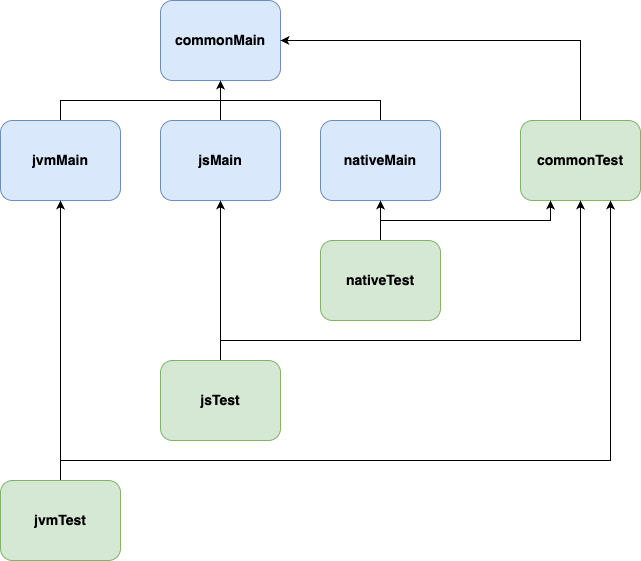
\includegraphics[width=0.95\textwidth]{charts/kmp-structure.drawio.png}
    \caption{Przykładowa struktura pojektu Kotlin Multiplatform [źródło:~opracowanie~własne]}
    \label{fig:kmp_project_structure}
\end{figure}

Następnie programista może utworzyć kolejne katalogi, które będą zawierać kod specyficzny dla docelowych platform.
Przykładowa struktura została przedstawiona na Rysunku \ref{fig:kmp_project_structure}, gdzie katalog commonMain jest wspóldzielony między JVM (jvmMain), JavaScript (jsMain) oraz platformy natywne (nativeMain).
Docelowe platformy (ang. targets) są deklarowane w konfiguracji Gradle \cite{kotlinMultiplatformDev}, a kod współdzielony jest przygotowywany wyłącznie dla nich.
Katalogi dla docelowych platform są wymagane, gdyż Kotlin nie zezwala na użycie specyficznych elementów danej platformy w katalogu współdzielonym.
Przykładem takiego elementu może być klasa ,,java.io.File'', która jest dostępna wyłącznie dla maszyny wirtualnej Javy.
Jej użycie w katalogu commonMain spowoduje błąd kompilacji.

Kotlin Multiplatform zawiera także integracje z testami oprogramowania.
Jest to szczególnie ważne dla tworzenia oprogramowania z wykorzystaniem AWS Lambda, gdzie testowanie może być skomplikowane (co było jednym z wniosków przeglądu literatury w Rozdziale \ref{chapter:przeglad_literatury}).
Testy dla kodu współdzielonego powinny być zapisane w katalogu ,,commonTest'', gdzie programista może użyć biblioteki kotlin.test \cite{kotlinMultiplatformDev}.
Następnie testy są uruchamiane dla każdej docelowej platformy.
Programista może także tworzyć przypadki testowe dla konkretnych platform, z użyciem technologii przez nie oferowanych.
Następuje tutaj analogiczne współdzielenie kodu jak dla katalogów ,,main'', co zostało także zawarte w Rysunku \ref{fig:kmp_project_structure}.

Specyficzne cechy Kotlina jak funkcjonalności języka, biblioteki czy projekt Kotlin Multiplatform mogą zapewnić znaczne wzrosty wydajności funkcji AWS Lambda.
Mimo, że Kotlin jest językiem wywodzącym się z Javy oferuje już możliwości, które mogą pozwolić na osiągnięcie niższych czasów odpowiedzi.
Dodatkowo, sposoby te nie zostały jeszcze przebadane. 
Dlatego Kotlin to obszar, który zasługuje na zawarcie go w badanich na temat wydajności AWS Lambda.

\section{Kotlin/JS}\label{chapter:kotlin_js}

\section{Kotlin/Native}\label{chapter:kotlin_native}

Bardzo skuteczną metodą optymalizacji wydajności może być rezygnacja z zarządzanych środowisk uruchomieniowych jak JVM.
Jedną z metod jest kompilacja do kodu natywnego, który uruchamiany jest bezpośrednio na systemie operacyjnym poza maszyną wirtualną.
Kotlin/Native oferuje zaawansową kompilację kodu Kotlin, który następnie może zostać uruchomiony w AWS Lambda z użyciem Amazon Linux.
W ramach rozdziału opisano sposób działania Kotlin/Native, jego możliwości i cechy, które mogą negatywnie wpłynąć na rozwój oprogramowania bezserwerowego.

Kluczowym elementami Kotlin/Native są kompilator oparty o LLVM oraz natywne implementacje bibliotek standardowych Kotlina \cite{kotlinlangKotlinDocs}.
Jak opisują Lattner i Adve \cite{1281665}, LLVM to framework kompilatora zaprojektowany do wspierania ciągłej i transparentnej analizy oraz transformacji programów.
Definiuje on wspólną, niskopoziomową reprezentację kodu w formie SSA (ang. Static Single Assignment) z systemem typów niezależnym od języka, co umożliwia implementację cech języków wysokiego poziomu. 
Głównym celem LLVM jest umożliwienie analizy i transformacji programu na różnych etapach jego życia, w tym w czasie kompilacji, linkowania, uruchomienia oraz w czasie bezczynności między uruchomieniami.
Jego użycie pozwala następnie na zbudowanie natywnych plików binarnych, które mogą zostać uruchomione bezpośrednio na docelowej platformie, dla której zostały skompilowane.
Wymaga to jednak dokładnego określenia systemu operacyjnego i architektury już w momencie kompilacji.

Kompilacja Kotlina do kodu natywnego otwiera przez KMP możliwość tworzenia samodzielnych programów wykonywalnych, które nie wymagają zewnętrznego środowiska uruchomieniowego.
Znajduje to zastosowanie w scenariuszach takich jak rozwój aplikacji mobilnych na platformę iOS, współdzielenie logiki biznesowej między różnymi platformami (np. Android i iOS) czy budowa narzędzi konsolowych.
Dlatego ważnym aspektem Kotlin/Native jest współdziałanie z istniejącym kodem natywnym.
Pozwala to na bezpośrednie wywoływanie funkcji z bibliotek napisanych w języku C, a na platformach firmy Apple również Objective-C \cite{kotlinlangKotlinDocs}.
Znacząco rozszerza to zakres dostępnych narzędzi i bibliotek, które mogą zostać użyte przez programistów.

Kotlin/Native oferuje wiele różnych platform docelowych, rozszerzając tym samym zakres zastosowań języka Kotlin.
Wśród wspieranych systemów docelowych znajdują się platformy Apple (takie jak macOS, iOS, watchOS, tvOS), Android, a także systemy z rodziny Windows oraz Linux \cite{kotlinlangKotlinDocs}.
Szczególnie istotnie dla usługi AWS Lambda są jednak platformy linuxowe.
Są to linuxX64 oraz linuxArm64, które pozwalają na uruchomienie kodu z użyciem odpowiednio architektur x86 oraz ARM.
Pozwala to następnie na ich bezpośrednie użycie w AWS Lambda, działającej bezpośrednio w systemie Amazon Linux.
Dzięki temu możliwa jest poprawa wydajności, szczególnie w aspekcie zimnych startów, które są znacznym wyzwaniem dla funkcji opartych o JVM.

Istotnym elementen funkcji bezserwerowych jest zarządzanie pamięcią, która wpływa bezpośrednio na koszty.
W przypadku Kotlin/Native, ewolucja modelu zarządzania pamięcią znacząco wpłynęła na jego użyteczność i możliwości optymalizacyjne.
Początkowa technologia ta opierała się na restrykcyjnym modelu z izolacją obiektów między wątkami \cite{kotlinlangKotlinDocs}.
Powodowało to skomplikowane zarządzanie stanem w operacjach współbieżnych.
Aktualnie, Kotlin/Native implementuje nowy menedżer pamięci.
Wprowadza on automatyczne zarządzanie pamięcią poprzez współbieżny, nieblokujący moduł zbierania śmieci (ang. garbage collector) \cite{kotlinlangKotlinDocs}.
Znacząco upraszcza to programowanie współbieżne, które teraz nie wymaga ręcznego zarządzania obiektami.
Mechanizm ten wprowadza intuicyjne współdzielenie stanu, które jest analogiczne do środowiska JVM, jednak bez konieczności kosztownej obsługi maszyny wirtualnej Java.

Mimo potencjalnych zysków w ramach wydajności, użycie Kotlin/Native może nieść utrudnienia w kontekście integracji z bibliotekami zewnętrznymi.
Język C nie jest oficjalnie wspierany jako język programowania AWS Lambda \cite{awsLambdaDeveloperGuide}, co wynika zapewne z jego niewielkiej popularności na tej platformie.
Współdziałanie z kodem natywnym w Kotlin/Native skupia się jednak na platformach klienckich, co nie musi być do końca użyteczne w zakresie AWS Lambda.
Amazon Web Services oferuje swoje SDK w języku C++, który nie jest jednak łatwo integrowalny z Kotlin/Native (w odróżnieniu od C i Objective-C).
Jest to ważny czynnik, który powinien być uwzględniony przez programistów projektujących aplikacje bezserwerowe.

% Plan
% 0. Wstęp

% 1. Jak to działa:
% - Opisać LLVM
% - Gdzie się głównie używa
% - Wspomnieć o interoperacyjności z C, Objective-C itp
% - Jakie platformy? (https://kotlinlang.org/docs/native-target-support.html#for-library-authors)

% 2. Zarządzanie pamięcią (https://kotlinlang.org/docs/native-memory-manager.html)

% 3. Wady - problem z dostępnością bibliotek
% - AWS SDK może poprzez C++ jednak może to wymagać większego nakładu pracy


\chapter{Wybrane metody optymalizacji}\label{chapter:wybrane_metody_optimalizacji}

% TODO: jakiś wstęp, typu jakich metod brakowało w przeglądzie. Podkreślić brak innych języków
\section{SnapStart}\label{chapter:snapstart}

Jednym z istotnych czynników wpływających na wydajność funkcji AWS Lambda implementowanych w ekosystemie Java jest zjawisko tzw. zimnego startu.
Wynika on z cyklu życia funkcji i etapu inicjalizacji (co zostało opisane w Rozdziale \ref{chapter:aws_lambda}).
W etap ten wchodzą procesy takie jak inicjalizacja maszyny wirtualnej Java czy uruchomienie statycznego kodu inicjującego \cite{awsLambdaDocs}.
W przypadku Javy zajmuje to więcej czasu niż dla innych języków (jak Python), co wydłuża zimne starty \cite{8605773}.
Znacząco oddziałuje to na wydajność funkcji, a może być szczególnie dotkliwe dla serwisów o niewielkiej aktywności.
W odpowiedzi na potrzebę minimalizacji tych negatywnych skutków Amazon Web Services wprowadziło mechanizm znany jako AWS Lambda SnapStart.
W ramach podrozdziału podjęto analizę tego rozwiązania w kontekście jego działania, zalet oraz ograniczeń. 

Mechanizm SnapStart istotnie modyfikuje tradycyjny cykl życia funkcji AWS Lambda.
Zasadnicza różnica polega na przeniesieniu kosztownego etapu inicjalizacji z momentu pierwszego wywołania funkcji na etap jej publikacji \cite{amazonSnapstartDeveloperGUide}.
Oznacza to, że inicjalizacja funkcji nie jest wykonywana w momencie zapytania użytkownika (co wywołuje zimny start), lecz w momencie wgrania nowej wersji funkcji (oraz kodu) przez programistę.
Inicjalizacja ta zawiera najdłuższe operacje dla rozwiązań Java jak utworzenie maszyny wirtualnej, załadowanie klas, czy wykonanie kodu inicjalizującego.
Następnie, tworzona jest zaszyfrowana ,,migawka'' (ang. snapshot) stanu pamięci i dysku w pełni gotowego środowiska wykonawczego.
Gdy funkcja jest następnie wywoływana po raz pierwszy, nie zachodzi już standardowy zimny start.
Zamiast tego środowisko jest odtwarzane z utworzonej migawki, co zostało przedstawione na Rysunku \ref{fig:aws_lambda_snapstart_process}.
Według dostawcy AWS metoda ta w optymalnych scenariuszach zmniejsza opóźnienie z kilku sekund do mniej niż sekundy \cite{amazonSnapstartDeveloperGUide}. 

\begin{figure}[h]
    \centering
    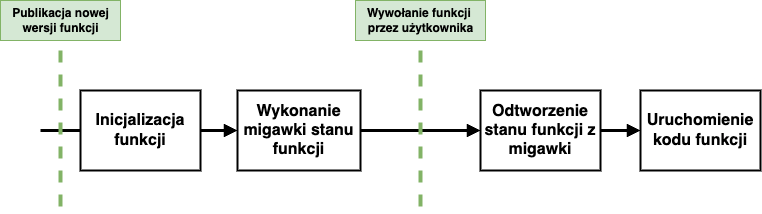
\includegraphics[width=0.95\textwidth]{charts/snapstart.png}
    \caption{Proces uruchomienia AWS Lambda z użyciem metody SnapStart [źródło:~opracowanie~własne]}
    \label{fig:aws_lambda_snapstart_process}
\end{figure}

Działanie tej metody jest technicznie możliwe dzięki użyciu środowiska wirtualizacji przez AWS Lambda.
Jak opisują Agache i inni autorzy \cite{246288} usługa Lambda do izolacji poszczególnych funkcji wykorzystuje dedykowane maszyny wirtualne typu microVM.
Są one zarządzane przez lekki monitor maszyn wirtualnych (ang. VMM) o nazwie Firecracker.
Posiada on cechy, które były kluczowe w minimalizacji problemu zimnego startu.
Po pierwsze, celowo rezygnuje on z emulacji zbędnych urządzeń (jak emulacja systemu BIOS czy rozbudowanych kontrolerów PCI) \cite{246288}.
Zmniejsza to złożoność i rozmiar stanu każdej maszyny wirtualnej. 
Dzięki temu wykonanie i odtworzenie migawki jest łatwiejsze.
Po drugie, Firecracker jest w pełni kontrolowany przez interfejs REST API \cite{246288}.
Umożliwia to precyzyjne zarządzanie całym cyklem życia każdej maszyny wirtualnej, włączając w to jej konfigurację, uruchomienie oraz zatrzymanie.
Pozwala to na określenie fazy inicjalizacji funkcji oraz wykonanie migawki w odpowiednim momencie.
Istotna jest również zapewniona przez Firecracker izolacja \cite{246288}, co gwarantuje bezpieczeństwo tworzenia i odtwarzania migawek.

Samo użycie metody SnapStart jest bardzo proste i nie wymaga od programisty dużego nakładu pracy.
Włączenie rozwiązania wymaga jedynie ustawienia odpowiedniej opcji podczas konfiguracji funkcji \cite{amazonSnapstartDeveloperGUide}.
Nie oznacza to jednak, że SnapStart jest odpowiedni dla wszystkich funkcji.
AWS podkreśla dwa typy aplikacji, które znacząco zyskają poprzez użycie SnapStart \cite{amazonSnapstartDeveloperGUide}.
Są nimi wrażliwe na opóźnienia interfejsy API i potoki przetwarzania danych.
Dodatkowo, metoda ta niesie za sobą pewne ograniczenia, które muszą zostać uwzględnione przed jej wdrożeniem.

Pierwszym aspektem jest kwestia unikalności stanu w funkcjach wykorzystujących SnapStart.
Jak analizują Brooker i inni autorzy \cite{brooker2021restoringuniquenessmicrovmsnapshots}, klonowanie migawek wprowadza fundamentalne wyzwanie związane z przywróceniem unikalności maszyn wirtualnych, co jest niezbędne do poprawnego generowania unikalnych identyfikatorów czy sekretów kryptograficznych.
Migawka zainicjowanego środowiska wykonywana jest jednorazowo, a następnie używana podczas wielu wywołań funkcji.
Może to stanowić duże zagrożenie dla programisty AWS Lambda, gdy potrzebuje on generować unikalne wartości jak identyfikatory (np. UUID) czy jednorazowe tokeny.
Narusza to znacznie poprawność logiki aplikacji oraz jej bezpieczeństwo.
Jedną z metod naprawy tego problemu jest generowanie wartości losowych wyłącznie w metodzie wywołującej funkcje (zamiast w bloku statycznym kodu) \cite{amazonSnapstartDeveloperGUide}.
Dodatkowo, ewentualne problemy z unikalnością funkcji SnapStart mogą zostać wykryte poprzez oprogramowanie SpotBugs \cite{SpotBugsProject}.
Narzędzie wykonuje statyczną analizę kodu, walidując go poprzez reguły zapewnione przez AWS.
Pozwala to programiście wykryć, a następnie naprawić fragmenty kodu powodujące problem z unikalnością.

Kolejnym istotnym wyzwaniem podczas rozwoju aplikacji z technologią SnapStart jest zarządzanie połączeniami sieciowymi \cite{amazonSnapstartDeveloperGUide}.
Połączenia nawiązane z zewnętrznymi usługami są standardową praktyką podczas tworzenia aplikacji AWS Lambda \cite{eismann2021reviewserverlessusecases}\cite{Ivanov_Petrova_2024}.
Problematyczne stają się jednak te połączenia sieciowe, które nawiązano podczas inicjalizacji funkcji. 
Ponieważ inicjalizacja odbywa się przed faktycznym przetworzeniem żądania użytkownika, upływający czas może sprawić, że w momencie odtworzenia funkcji połączenia te nie będą już aktywne.
Praktyką zalecaną przez AWS jest ponowne nawiązywanie lub dokładna walidacja istniejących połączeń \cite{amazonSnapstartDeveloperGUide}.
Powinno to być wykonane bezpośrednio w metodzie wywołującej funkcje lub z wykorzystaniem metody ,,afterRestore''.
Metoda ta jest wywoływana bezpośrednio po odtworzeniu migawki stanu funkcji.

Strategicznym czynnikiem usług bezserwerowych są koszty, zatem powinny być one uwzględnione także przed użyciem SnapStart.
Zgodnie z dokumentacją Amazon Web Services \cite{amazonSnapstartDeveloperGUide}, użycie SnapStart dla środowisk uruchomieniowych Java nie wiążą się z dodatkowymi kosztami.
Koszt wykonania funkcji z włączonym SnapStart nadal bazuje na standardowych rozliczeniach.
Składa się na niego liczba przetworzonych żądań oraz łączny czas trwania wykonań.

Podsumowując, mechanizm SnapStart stanowi prostą w aktywacji metodę redukcji czasu zimnych startów.
Sam mechanizm opiera się na wcześniejszym wykonaniu fazy inicjacji funkcji, a następnie wykonania migawki stanu.
W momencie wywołania funkcji stan ten może zostać odtworzony.
Znaczącą korzyścią metody jest brak dodatkowych kosztów.
Wiąże się ona jednak z istotnymi utrudnieniami (jak zarządzanie połączeniami sieciowymi i problem z unikalnością stanu).
Powinny być one uwzględnione przez programistę przed użyciem narzędzia.
\section{GraalVM}\label{chapter:graalvm}

Ważnym obszarem badań nad optymalizacją Javy i jej użycia w AWS Lambda, są technologie pozwalające na zmianę sposobu kompilacji i uruchamiana aplikacji.
Jedną z technologii, które zyskusje na popularności w tym zakresie, jest GraalVM.
Jest to możliwe m.in. dzięki użyciu kompilatora JIT (ang. Just-In-Time) w połączeniu z kompilacją AOT (ang. Ahead-Of-Time) \cite{8756917}.
GraalVM oferuje zaawansowaną architekturę pozwalającą na kompilację i uruchomienie aplikacji w postaci obrazów natywnych.
Stanowi to alternatywę dla klasycznej maszyny wirtualnej Javy, a dodatkowo skupia się na jej wydajności.
Poniższy podrozdział poświęcono analizie działania omawianego rozwiązania, jego zalet i słabych stron.

Kluczowym mechanizmem GraalVM jest kompilacja AOT (ang. Ahead-Of-Time) do postaci tzw. obrazów natywnych (ang. native images) \cite{8756917}.
Ma to bezpośredni wpływ na wydajność działania aplikacji.
W modelu tradycyjnym, kod bajtowy Java jest interpretowany i kompilowany dynamicznie przez maszynę wirtualną w trakcie działania aplikacji.
Podejście AOT przenosi znaczną część z tych operacji na etap budowania artefaktu. 
Istotnym elementem tego procesu jest agresywna, statyczna analiza kodu \cite{9245290}, w celu identyfikacji osiągalnych w trakcie działania części.
Pozwala to na odrzucenie nieużywanych fragmentów kodu (np. z używanych bibliotek), co pozwala na zmniejszenie wielkości obrazu natywnego.
Aspekt ten może być kluczowy w kontekście AWS Lambda, ze względu na wpływ wielkości artefaktu na wydajność \cite{8116416}.
Po analizie kodu, dokonywana jest inicjalizacja klas, a stan aplikacji, w tym częściowo zainicjalizowana sterta, jest utrwalany.
W celu lepszej optymalizacji, operacje te są powtarzane, co zostało przedstawione na Rysunku \ref{fig:graalvm_build_process}.

Jako wynik kompilacji powstaje samodzielny, zoptymalizowany plik binarny.
Nie wymaga on do uruchomienia pełnej maszyny wirtualnej Java, a jedynie minimalnego środowiska wykonawczego dostarczanego przez SubstrateVM, będącego częścią GraalVM \cite{8756917}.
Różnica ta ma fundamentalne znaczenie w kontekście wydajności AWS Lambda.
Eliminowana jest konieczność wykonywania czasochłonnych operacji typowych dla startu tradycyjnej maszyny wirtualnej Java, takich jak ładowanie klas czy jej inicjalizacja.
Wszystkie te zadania zostały już wykonane wcześniej, w procesie budowy obrazu natywnego.
Dzięki temu tworzona przez programistę funkcja AWS Lambda nie będzie operować w zarządzanym środowisku Java.
Zamiast tego, usługi muszą opierać się o niestandardowe środowiska wykonawcze, oferujące wyłącznie system operacyjny (Amazon Linux 2023 lub Amazon Linux 2) \cite{awsLambdaDeveloperGuide}.
Ich użycie pozwala także na realizację drugiej zalety GraalVM, czyli redukcji zapotrzebowania na pamięć operacyjną \cite{9245290}.

Pomimo pozytywnego wpływu na wydajność, zastosowanie kompilacji AOT w GraalVM wiąże się także z ograniczeniami.
Jednym z nich jest obsługa dynamicznych cech Javy, takich jak refleksja (ang. reflection), dynamiczne proxy, serializacja czy natywny interfejs Java (JNI)
Wynika to z faktu użycia agresywnej statycznej analizy kodu.
Napotyka ona trudności w przewidzeniu wszystkich dynamicznie ładowanych klas, pól i metod, które nie są jawnie osiągalne w kodzie źródłowym.
Problem ten wymaga użycia dodatkowych mechanizmów GraalVM \cite{graalvm-reflection-jdk21}.
Polegają one na przygotowaniu dodatkowych metadanych dla klas, co wymaga jednak dodatkowej obsługi.

\begin{figure}
    \centering
    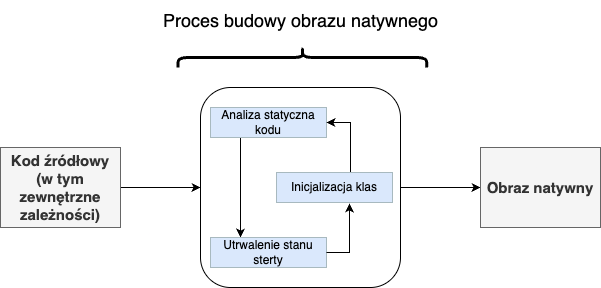
\includegraphics[width=0.95\textwidth]{charts/graalvm-build-process.drawio.png}
    \caption{Uproszczony proces budowy obrazu natywnego GraalVM [źródło:~opracowanie~własne]}
    \label{fig:graalvm_build_process}
\end{figure}

Kolejnym aspektem, który może negatywnie wpłynąć na rozwój oprogramowania przy użyciu GraalVM, jest czasochłonność procesu kompilacji.
Generowanie w pełni zoptymalizowanego obrazu natywnego jest operacją bardziej złożoną niż standardowa kompilacja kodu Javy do postaci bajtowej.
W praktyce oznacza to, że proces budowania artefaktu dla funkcji AWS Lambda może trwać odczuwalnie dłużej.
Może mieć to znaczący wpływ na rozwój oprogramowania, szczególnie w przypadku częstych iteracji i tworzenia nowych wersji funkcji.
Dłuższy czas kompilacji może także wpłynąć na ogólną efektywność procesów ciągłej integracji i ciągłego dostarczania (ang. CI/CD).

Jednym z sposobów poprawy doświadczeń programistów przy pracy z GraalVM, jest użycie odpowiednich frameworków.
Jednym z nich jest Quarkus \cite{9245290}, który został zaprojektowany z myślą o środowiskach chmurowych.
Kluczową cechą Quarkusa jest przeniesienie jak największej liczby operacji inicjalizacyjnych i konfiguracyjnych na etap budowania aplikacji.
Obejmuje to między innymi wstrzykiwanie zależności, przetwarzanie adnotacji oraz konfigurację rozszerzeń. 
Dzięki temu, w czasie budowania obrazu natywnego, Quarkus jest w stanie przeprowadzić szczegółową analizę aplikacji.
Poprzez użycie odpowiednich annotacji pozwala on na oznaczenie klas niezbędnych dla mechanizmów refleksji czy proxy \cite{quarkus-docs}.
Dzięki temu jest on w stanie automatycznie wygenerować niezbędne metadane dla klas.
Dane te następnie pozwalają na użycie wspomnianych mechanizmów w GraalVM.
Innymi, konkurencyjnymi do Quarkusa frameworkami, które oferują wsparcie dla obrazów natywnych są Helidon i Micronaut \cite{9245290}.
Ich popularność wskazuje na wysokie zainteresowanie takimi technologiami w społeczności programistów Java, dlatego jest to interesujący kierunek rozwoju dla funkcji AWS Lambda.

\section{Kotlin}\label{chapter:kotlin_multiplatform}

W ramach systematycznego przeglądu literatury (przedstawionego w Rozdziale \ref{chapter:przeglad_literatury}) zauważono, że aktualne badania skupiają się wyłącznie na języku Java.
Pomijają one jednak inne języki z ekosystemu Java, także oparte o maszynę wirtualną Java (ang. JVM).
Tymczasem na popularności zyskują alternatywne języki ekosystemu Javy.
Wśród nich na szczególną uwagę zasługuje Kotlin, rozwijany przez firmę JetBrains.
Jest on oficjalnie wspierany przez Google jako język programowania dla platformy Android, co wskazuje na jego solidne zastosowanie w tych systemach.
Coraz większe uznanie zyskuje także jako działający po stronie serwera. 
Dlatego język ten jest interesującym obszarem badań w kontekście AWS Lambda.
W tym rozdziale przedstawiony zostanie język programowania Kotlin, w tym jego zastosowanie w kontekście funkcji AWS Lambda.

Jednym z kluczowych czynników, które zwiększają popularność Kotlina, jest jego łatwa nauka przez programistów Javy.
Dodatkowo, istnieje możliwość łatwej intergracji kodu napisanego w Kotlinie z istniejącym oprogramowaniem Java \cite{kotlinlangKotlinDocs}.
Te cechy czynią go interesującym kandydatem do analizy w kontekście optymalizacji wydajności rozwiązań dla usługi AWS Lambda. 
Dla zespołów programistycznych może stanowić on wartościowe rozszerzenie dotychczasowych możliwości. 
Kotlin oferuje bowiem alternatywę lub uzupełnienie dla tradycyjnie stosowanej Javy.

Kwestia wydajności Kotlina w porównaniu do Javy jest przedmiotem dyskusji. 
Jednak badania dotyczą najczęściej ich zastosowań w kontekście aplikacji mobilnych.
Gajek i inni autorzy \cite{Gajek_Plechawska-Wójcik_2024} przeanalizowali wydajność obu języków, poprzez użycie gry mobilnej uruchomionej na systemie Android.
Wykazali oni, że w testowanym scenariuszu Java osiągnęła nieznacznie lepszą wydajność pod względem zużycia zasobów CPU i RAM.
Było to jednak zastosowanie mobilne, a same różnice nie były znaczne.
Należy jednak podkreślić, że warunki mobilne mogą być inne niż w systemach działających w usłudze AWS Lambda.
Sam język Kotlin posiada mechanizmy, które mogą pozytywnie wpłynąć na wydajność.

Funkcje inline (ang. inline functions) w Kotlinie mogą przyczynić się do redukcji narzutu wydajności podczas wywołań funkcji.
Mechanizm ten polega na wstawieniu kodu ciała funkcji bezpośrednio w miejsce jej wywołania \cite{kotlinlangKotlinDocs}.
Jest to wykonywane w momencie kompilacji, a programista może określić, które funkcje powinny być w ten sposób optymalizowane.
Eliminuje to koszt ich wywołania, co jest szczególnie przydatne w przypadku małych, często używanych funkcji.
Dodatkowo, język pozwala na przekazywanie funkcji jako parametrów, na przykład w kolekcjach i metodach jak filtrowanie.
W tych sytuacjach użycie funkcji inline może znacząco zmniejszyć liczbę operacji.
Pozytywny wpływ mechanizmu inline został przedstawiony przez Bergstrom i innych autorów \cite{DBLP:journals/corr/BergstromFRS13}, gdzie jego użycie zmniejszyło czas wykonywania programów nawet do 8\%.

Innym istotnym elementem Kotlina wspierającym wydajność są korutyny (ang. coroutines).
Mogą być one użyteczne zwłaszcza w kontekście operacji wejścia-wyjścia (I/O).
Systemy oparte o usługę AWS Lambda często integrowane są z zewnętrznymi serwisami (co zostało zauważone w ramach przeglądu literatury w Rozdziale \ref{chapter:przeglad_literatury}).
Wymaga to komunikacji opartej o operacje sieciowe.
Tradycyjne podejście oparte na wątkach może konsumować dużą ilość zasobów serwera i prowadzić do blokowania wykonania.
Korutyny pozwalają na pisanie asynchronicznego, nieblokującego kodu w sposób bardziej sekwencyjny i czytelny \cite{kotlinlangKotlinDocs}.
Na lepszą wydajność korutyn w porównaniu z tradycyjnymi wątkami wskazali Beronić i inni autorzy \cite{9803765}.

Implementacja mechanizmów poprawiających wydajność w języku programowania, pozwala następnie na ich użycie w bibliotekach, które są wykorzystywane przez programistów.
Język Kotlin oferuje ciekawy ekosystem bibliotek, przeznaczonych na przykład do tworzenia aplikacji działających po stronie serwera.
Są to biblioteki jak http4k czy ktor.
Ktor to framework zaprojektowany do budowy asynchronicznych aplikacji serwerowych i klienckich, rozwijany przez firmę JetBrains.
Jest on oparty w pełni o język Kotlin, a jego kluczową cechą jest natywne wsparcie dla korutyn.
Z kolei http4k kładzie nacisk na prostotę i minimalizm.
Architektura http4k opiera się na koncepcji funkcji jako podstawowych bloków aplikacji \cite{http4kCoreDocs}, co naturalnie współgra z modelem serverless i AWS Lambda.
Samo narzędzie rezyguje z mechanizmów refleksji \cite{http4kCoreDocs}, co może mieć pozytywny wpływ na wydajność.

Rosnące znaczenie Kotlin dostrzega także Amazon Web Service, które oferuje bibliotekę AWS SDK dla Kotlina \cite{awsSDKForKotlinDeveloperGuide}.
Jej celem jest zapewnienie programistom możliwości interakcji z usługami AWS w sposób naturalny dla tego języka.
SDK ten został zaprojektowany od podstaw z myślą o Kotlinie, co przejawia się między innymi w wykorzystaniu korutyn do obsługi operacji asynchronicznych.

Duży wpływ na wydajność funkcji AWS Lambda ma wybrany język programowania \cite{8605773}\cite{Cordingly2020704}.
Wynika to na przykład z różnych przypadków biznesowych i operacji, które muszą wykonywać.
Mimo to, często muszą one dzielić wspólny kod \cite{8116416}, co wskazuje na potrzebę wykorzystania mechanizmów, które to umożliwą.
Z tego powodu bardzo interesującą dla AWS Lambda i jej wydajności, może okazać się inicjatywa Kotlin Multiplatform.
KMP (Kotlin Multiplatform) to projekt, który powstał w szczególności dla aplikacji mobilnych.
Pozwala on na kompilację lub translację tego samego kodu Kotlin do użycia na różnych platformach.
Mogą to być na przykład Android, iOS, aplikacje desktopowe (JVM) lub webowe (JavaScript, Web Assembly) \cite{kotlinlangKotlinDocs}.
Oferuje to możliwość dzielenia kodu (np. logiki biznesowej) pomiędzy różnymi platformami, jednak przy możliwości zachowania natywnych komponentów widoku.

Mimo głównego przypadku użycia jakim są aplikacje klienckie, Kotlin Multiplatform może być obiecującym rozwiązaniem dla AWS Lambda.
Po pierwsze oferuje on możliwość translacji kodu Kotlin do JavaScript oraz kompilację do natywnych plików binarnych (opcje te zostaną przedstawione jako osobne metody w kolejnych rozdziałach).
Pozwala to na ominięcie różnych niedogodności wynikających z użycia maszyny wirtualnej Javy.
Jednak zachowane są przy tym zalety języka oraz wspiera to użycie już istniejących umiejętności programistów języków rodziny JVM.
Po drugie, kod w KMP może być dzielony pomiędzy platformami.
Umożliwia to bardzo elastyczny wybór środowiska uruchomieniowego AWS Lambda w ramach pojedynczego systemu.
Jednocześnie, część kodu może być współdzielona między wszystkie funkcje niezależnie od wybranej platformy.
Może to na przykład oznaczać, że klasy implementujące pewne struktury oraz zasady wynikające z reguł biznesowych, będą mogły być używane przez funkcje działające zarówno poprzez JavaScript, JVM, jak i natywne pliki binarne. 

Jednym z czynników, które mogą być modyfikowane już podczas działania usług AWS Lambda jest pamięć.
Jej rozmiar może być dostosowywany w zależności od wydajności monitorowanej funkcji.
Użycie Kotlin Multiplatform pozwala na rozszerzenie tej metody.
W zależności od obserwowanych parametrów (jak czas odpowiedzi lub opóźnienia zimnych startów) możliwe jest ponowne wykorzystanie tego samego kodu i budowa funkcji działającej na innej platformie.
Przykładowo, po wdrożeniu funkcji działającej z użyciem JVM, może pojawić się potrzeba redukcji czasu zimnych startów.
W takim wypadku Kotlin Multiplatform umożliwia translację kodu do JavaScript, który pozwoli na redukcję czasu inicjalizacji AWS Lambda.

Współdzielenie kodu pomiędzy platformami jest możliwe dzięki strukturze, którą oferuje Kotlin Multiplatform.
Została ona opisana przez firmę JetBrains w ramach dokumentacji KMP \cite{kotlinMultiplatformDev}.
Jej głównym elementem jest katalog ,,commonMain'', który jest współdzielony pomiędzy wszystkimi platformami.
Kompilator używa kodu współdzielonego jako dane wejściowe, aby w rezultacie utworzyć zestaw plików binarnych specyficznych dla danej platformy.
Mogą to być na przykład pliki .class dla maszyny wirtualnej Javy, czy natywne pliki wykonywalne (np. dla platformy Linux).

\begin{figure}[h]
    \centering
    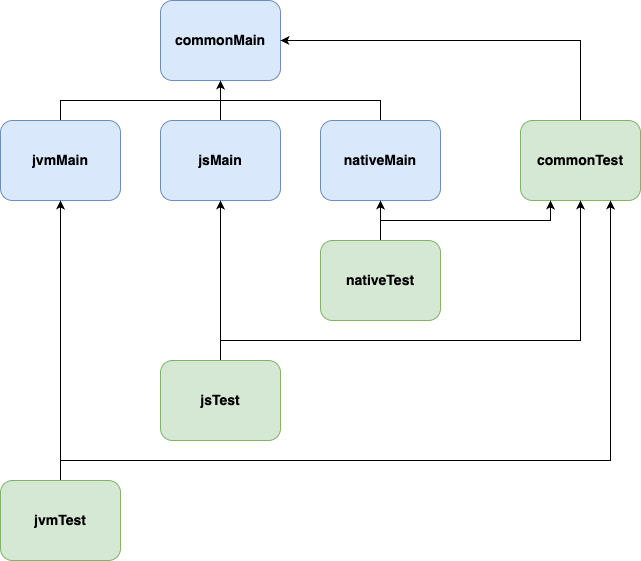
\includegraphics[width=0.95\textwidth]{charts/kmp-structure.drawio.png}
    \caption{Przykładowa struktura pojektu Kotlin Multiplatform [źródło:~opracowanie~własne]}
    \label{fig:kmp_project_structure}
\end{figure}

Następnie programista może utworzyć kolejne katalogi, które będą zawierać kod specyficzny dla docelowych platform.
Przykładowa struktura została przedstawiona na Rysunku \ref{fig:kmp_project_structure}, gdzie katalog commonMain jest wspóldzielony między JVM (jvmMain), JavaScript (jsMain) oraz platformy natywne (nativeMain).
Docelowe platformy (ang. targets) są deklarowane w konfiguracji Gradle \cite{kotlinMultiplatformDev}, a kod współdzielony jest przygotowywany wyłącznie dla nich.
Katalogi dla docelowych platform są wymagane, gdyż Kotlin nie zezwala na użycie specyficznych elementów danej platformy w katalogu współdzielonym.
Przykładem takiego elementu może być klasa ,,java.io.File'', która jest dostępna wyłącznie dla maszyny wirtualnej Javy.
Jej użycie w katalogu commonMain spowoduje błąd kompilacji.

Kotlin Multiplatform zawiera także integracje z testami oprogramowania.
Jest to szczególnie ważne dla tworzenia oprogramowania z wykorzystaniem AWS Lambda, gdzie testowanie może być skomplikowane (co było jednym z wniosków przeglądu literatury w Rozdziale \ref{chapter:przeglad_literatury}).
Testy dla kodu współdzielonego powinny być zapisane w katalogu ,,commonTest'', gdzie programista może użyć biblioteki kotlin.test \cite{kotlinMultiplatformDev}.
Następnie testy są uruchamiane dla każdej docelowej platformy.
Programista może także tworzyć przypadki testowe dla konkretnych platform, z użyciem technologii przez nie oferowanych.
Następuje tutaj analogiczne współdzielenie kodu jak dla katalogów ,,main'', co zostało także zawarte w Rysunku \ref{fig:kmp_project_structure}.

Specyficzne cechy Kotlina jak funkcjonalności języka, biblioteki czy projekt Kotlin Multiplatform mogą zapewnić znaczne wzrosty wydajności funkcji AWS Lambda.
Mimo, że Kotlin jest językiem wywodzącym się z Javy oferuje już możliwości, które mogą pozwolić na osiągnięcie niższych czasów odpowiedzi.
Dodatkowo, sposoby te nie zostały jeszcze przebadane. 
Dlatego Kotlin to obszar, który zasługuje na zawarcie go w badanich na temat wydajności AWS Lambda.

\section{Kotlin/JS}\label{chapter:kotlin_js}

\section{Kotlin/Native}\label{chapter:kotlin_native}

Bardzo skuteczną metodą optymalizacji wydajności może być rezygnacja z zarządzanych środowisk uruchomieniowych jak JVM.
Jedną z metod jest kompilacja do kodu natywnego, który uruchamiany jest bezpośrednio na systemie operacyjnym poza maszyną wirtualną.
Kotlin/Native oferuje zaawansową kompilację kodu Kotlin, który następnie może zostać uruchomiony w AWS Lambda z użyciem Amazon Linux.
W ramach rozdziału opisano sposób działania Kotlin/Native, jego możliwości i cechy, które mogą negatywnie wpłynąć na rozwój oprogramowania bezserwerowego.

Kluczowym elementami Kotlin/Native są kompilator oparty o LLVM oraz natywne implementacje bibliotek standardowych Kotlina \cite{kotlinlangKotlinDocs}.
Jak opisują Lattner i Adve \cite{1281665}, LLVM to framework kompilatora zaprojektowany do wspierania ciągłej i transparentnej analizy oraz transformacji programów.
Definiuje on wspólną, niskopoziomową reprezentację kodu w formie SSA (ang. Static Single Assignment) z systemem typów niezależnym od języka, co umożliwia implementację cech języków wysokiego poziomu. 
Głównym celem LLVM jest umożliwienie analizy i transformacji programu na różnych etapach jego życia, w tym w czasie kompilacji, linkowania, uruchomienia oraz w czasie bezczynności między uruchomieniami.
Jego użycie pozwala następnie na zbudowanie natywnych plików binarnych, które mogą zostać uruchomione bezpośrednio na docelowej platformie, dla której zostały skompilowane.
Wymaga to jednak dokładnego określenia systemu operacyjnego i architektury już w momencie kompilacji.

Kompilacja Kotlina do kodu natywnego otwiera przez KMP możliwość tworzenia samodzielnych programów wykonywalnych, które nie wymagają zewnętrznego środowiska uruchomieniowego.
Znajduje to zastosowanie w scenariuszach takich jak rozwój aplikacji mobilnych na platformę iOS, współdzielenie logiki biznesowej między różnymi platformami (np. Android i iOS) czy budowa narzędzi konsolowych.
Dlatego ważnym aspektem Kotlin/Native jest współdziałanie z istniejącym kodem natywnym.
Pozwala to na bezpośrednie wywoływanie funkcji z bibliotek napisanych w języku C, a na platformach firmy Apple również Objective-C \cite{kotlinlangKotlinDocs}.
Znacząco rozszerza to zakres dostępnych narzędzi i bibliotek, które mogą zostać użyte przez programistów.

Kotlin/Native oferuje wiele różnych platform docelowych, rozszerzając tym samym zakres zastosowań języka Kotlin.
Wśród wspieranych systemów docelowych znajdują się platformy Apple (takie jak macOS, iOS, watchOS, tvOS), Android, a także systemy z rodziny Windows oraz Linux \cite{kotlinlangKotlinDocs}.
Szczególnie istotnie dla usługi AWS Lambda są jednak platformy linuxowe.
Są to linuxX64 oraz linuxArm64, które pozwalają na uruchomienie kodu z użyciem odpowiednio architektur x86 oraz ARM.
Pozwala to następnie na ich bezpośrednie użycie w AWS Lambda, działającej bezpośrednio w systemie Amazon Linux.
Dzięki temu możliwa jest poprawa wydajności, szczególnie w aspekcie zimnych startów, które są znacznym wyzwaniem dla funkcji opartych o JVM.

Istotnym elementen funkcji bezserwerowych jest zarządzanie pamięcią, która wpływa bezpośrednio na koszty.
W przypadku Kotlin/Native, ewolucja modelu zarządzania pamięcią znacząco wpłynęła na jego użyteczność i możliwości optymalizacyjne.
Początkowa technologia ta opierała się na restrykcyjnym modelu z izolacją obiektów między wątkami \cite{kotlinlangKotlinDocs}.
Powodowało to skomplikowane zarządzanie stanem w operacjach współbieżnych.
Aktualnie, Kotlin/Native implementuje nowy menedżer pamięci.
Wprowadza on automatyczne zarządzanie pamięcią poprzez współbieżny, nieblokujący moduł zbierania śmieci (ang. garbage collector) \cite{kotlinlangKotlinDocs}.
Znacząco upraszcza to programowanie współbieżne, które teraz nie wymaga ręcznego zarządzania obiektami.
Mechanizm ten wprowadza intuicyjne współdzielenie stanu, które jest analogiczne do środowiska JVM, jednak bez konieczności kosztownej obsługi maszyny wirtualnej Java.

Mimo potencjalnych zysków w ramach wydajności, użycie Kotlin/Native może nieść utrudnienia w kontekście integracji z bibliotekami zewnętrznymi.
Język C nie jest oficjalnie wspierany jako język programowania AWS Lambda \cite{awsLambdaDeveloperGuide}, co wynika zapewne z jego niewielkiej popularności na tej platformie.
Współdziałanie z kodem natywnym w Kotlin/Native skupia się jednak na platformach klienckich, co nie musi być do końca użyteczne w zakresie AWS Lambda.
Amazon Web Services oferuje swoje SDK w języku C++, który nie jest jednak łatwo integrowalny z Kotlin/Native (w odróżnieniu od C i Objective-C).
Jest to ważny czynnik, który powinien być uwzględniony przez programistów projektujących aplikacje bezserwerowe.

% Plan
% 0. Wstęp

% 1. Jak to działa:
% - Opisać LLVM
% - Gdzie się głównie używa
% - Wspomnieć o interoperacyjności z C, Objective-C itp
% - Jakie platformy? (https://kotlinlang.org/docs/native-target-support.html#for-library-authors)

% 2. Zarządzanie pamięcią (https://kotlinlang.org/docs/native-memory-manager.html)

% 3. Wady - problem z dostępnością bibliotek
% - AWS SDK może poprzez C++ jednak może to wymagać większego nakładu pracy


\chapter{Wybrane metody optymalizacji}\label{chapter:wybrane_metody_optimalizacji}

% TODO: jakiś wstęp, typu jakich metod brakowało w przeglądzie. Podkreślić brak innych języków
\section{SnapStart}\label{chapter:snapstart}

Jednym z istotnych czynników wpływających na wydajność funkcji AWS Lambda implementowanych w ekosystemie Java jest zjawisko tzw. zimnego startu.
Wynika on z cyklu życia funkcji i etapu inicjalizacji (co zostało opisane w Rozdziale \ref{chapter:aws_lambda}).
W etap ten wchodzą procesy takie jak inicjalizacja maszyny wirtualnej Java czy uruchomienie statycznego kodu inicjującego \cite{awsLambdaDocs}.
W przypadku Javy zajmuje to więcej czasu niż dla innych języków (jak Python), co wydłuża zimne starty \cite{8605773}.
Znacząco oddziałuje to na wydajność funkcji, a może być szczególnie dotkliwe dla serwisów o niewielkiej aktywności.
W odpowiedzi na potrzebę minimalizacji tych negatywnych skutków Amazon Web Services wprowadziło mechanizm znany jako AWS Lambda SnapStart.
W ramach podrozdziału podjęto analizę tego rozwiązania w kontekście jego działania, zalet oraz ograniczeń. 

Mechanizm SnapStart istotnie modyfikuje tradycyjny cykl życia funkcji AWS Lambda.
Zasadnicza różnica polega na przeniesieniu kosztownego etapu inicjalizacji z momentu pierwszego wywołania funkcji na etap jej publikacji \cite{amazonSnapstartDeveloperGUide}.
Oznacza to, że inicjalizacja funkcji nie jest wykonywana w momencie zapytania użytkownika (co wywołuje zimny start), lecz w momencie wgrania nowej wersji funkcji (oraz kodu) przez programistę.
Inicjalizacja ta zawiera najdłuższe operacje dla rozwiązań Java jak utworzenie maszyny wirtualnej, załadowanie klas, czy wykonanie kodu inicjalizującego.
Następnie, tworzona jest zaszyfrowana ,,migawka'' (ang. snapshot) stanu pamięci i dysku w pełni gotowego środowiska wykonawczego.
Gdy funkcja jest następnie wywoływana po raz pierwszy, nie zachodzi już standardowy zimny start.
Zamiast tego środowisko jest odtwarzane z utworzonej migawki, co zostało przedstawione na Rysunku \ref{fig:aws_lambda_snapstart_process}.
Według dostawcy AWS metoda ta w optymalnych scenariuszach zmniejsza opóźnienie z kilku sekund do mniej niż sekundy \cite{amazonSnapstartDeveloperGUide}. 

\begin{figure}[h]
    \centering
    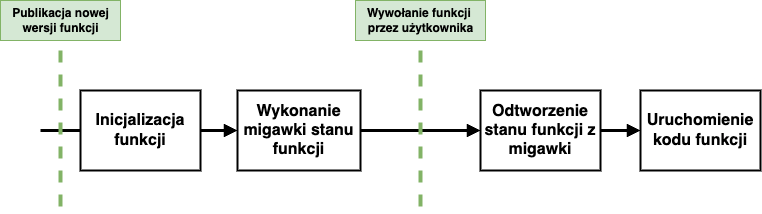
\includegraphics[width=0.95\textwidth]{charts/snapstart.png}
    \caption{Proces uruchomienia AWS Lambda z użyciem metody SnapStart [źródło:~opracowanie~własne]}
    \label{fig:aws_lambda_snapstart_process}
\end{figure}

Działanie tej metody jest technicznie możliwe dzięki użyciu środowiska wirtualizacji przez AWS Lambda.
Jak opisują Agache i inni autorzy \cite{246288} usługa Lambda do izolacji poszczególnych funkcji wykorzystuje dedykowane maszyny wirtualne typu microVM.
Są one zarządzane przez lekki monitor maszyn wirtualnych (ang. VMM) o nazwie Firecracker.
Posiada on cechy, które były kluczowe w minimalizacji problemu zimnego startu.
Po pierwsze, celowo rezygnuje on z emulacji zbędnych urządzeń (jak emulacja systemu BIOS czy rozbudowanych kontrolerów PCI) \cite{246288}.
Zmniejsza to złożoność i rozmiar stanu każdej maszyny wirtualnej. 
Dzięki temu wykonanie i odtworzenie migawki jest łatwiejsze.
Po drugie, Firecracker jest w pełni kontrolowany przez interfejs REST API \cite{246288}.
Umożliwia to precyzyjne zarządzanie całym cyklem życia każdej maszyny wirtualnej, włączając w to jej konfigurację, uruchomienie oraz zatrzymanie.
Pozwala to na określenie fazy inicjalizacji funkcji oraz wykonanie migawki w odpowiednim momencie.
Istotna jest również zapewniona przez Firecracker izolacja \cite{246288}, co gwarantuje bezpieczeństwo tworzenia i odtwarzania migawek.

Samo użycie metody SnapStart jest bardzo proste i nie wymaga od programisty dużego nakładu pracy.
Włączenie rozwiązania wymaga jedynie ustawienia odpowiedniej opcji podczas konfiguracji funkcji \cite{amazonSnapstartDeveloperGUide}.
Nie oznacza to jednak, że SnapStart jest odpowiedni dla wszystkich funkcji.
AWS podkreśla dwa typy aplikacji, które znacząco zyskają poprzez użycie SnapStart \cite{amazonSnapstartDeveloperGUide}.
Są nimi wrażliwe na opóźnienia interfejsy API i potoki przetwarzania danych.
Dodatkowo, metoda ta niesie za sobą pewne ograniczenia, które muszą zostać uwzględnione przed jej wdrożeniem.

Pierwszym aspektem jest kwestia unikalności stanu w funkcjach wykorzystujących SnapStart.
Jak analizują Brooker i inni autorzy \cite{brooker2021restoringuniquenessmicrovmsnapshots}, klonowanie migawek wprowadza fundamentalne wyzwanie związane z przywróceniem unikalności maszyn wirtualnych, co jest niezbędne do poprawnego generowania unikalnych identyfikatorów czy sekretów kryptograficznych.
Migawka zainicjowanego środowiska wykonywana jest jednorazowo, a następnie używana podczas wielu wywołań funkcji.
Może to stanowić duże zagrożenie dla programisty AWS Lambda, gdy potrzebuje on generować unikalne wartości jak identyfikatory (np. UUID) czy jednorazowe tokeny.
Narusza to znacznie poprawność logiki aplikacji oraz jej bezpieczeństwo.
Jedną z metod naprawy tego problemu jest generowanie wartości losowych wyłącznie w metodzie wywołującej funkcje (zamiast w bloku statycznym kodu) \cite{amazonSnapstartDeveloperGUide}.
Dodatkowo, ewentualne problemy z unikalnością funkcji SnapStart mogą zostać wykryte poprzez oprogramowanie SpotBugs \cite{SpotBugsProject}.
Narzędzie wykonuje statyczną analizę kodu, walidując go poprzez reguły zapewnione przez AWS.
Pozwala to programiście wykryć, a następnie naprawić fragmenty kodu powodujące problem z unikalnością.

Kolejnym istotnym wyzwaniem podczas rozwoju aplikacji z technologią SnapStart jest zarządzanie połączeniami sieciowymi \cite{amazonSnapstartDeveloperGUide}.
Połączenia nawiązane z zewnętrznymi usługami są standardową praktyką podczas tworzenia aplikacji AWS Lambda \cite{eismann2021reviewserverlessusecases}\cite{Ivanov_Petrova_2024}.
Problematyczne stają się jednak te połączenia sieciowe, które nawiązano podczas inicjalizacji funkcji. 
Ponieważ inicjalizacja odbywa się przed faktycznym przetworzeniem żądania użytkownika, upływający czas może sprawić, że w momencie odtworzenia funkcji połączenia te nie będą już aktywne.
Praktyką zalecaną przez AWS jest ponowne nawiązywanie lub dokładna walidacja istniejących połączeń \cite{amazonSnapstartDeveloperGUide}.
Powinno to być wykonane bezpośrednio w metodzie wywołującej funkcje lub z wykorzystaniem metody ,,afterRestore''.
Metoda ta jest wywoływana bezpośrednio po odtworzeniu migawki stanu funkcji.

Strategicznym czynnikiem usług bezserwerowych są koszty, zatem powinny być one uwzględnione także przed użyciem SnapStart.
Zgodnie z dokumentacją Amazon Web Services \cite{amazonSnapstartDeveloperGUide}, użycie SnapStart dla środowisk uruchomieniowych Java nie wiążą się z dodatkowymi kosztami.
Koszt wykonania funkcji z włączonym SnapStart nadal bazuje na standardowych rozliczeniach.
Składa się na niego liczba przetworzonych żądań oraz łączny czas trwania wykonań.

Podsumowując, mechanizm SnapStart stanowi prostą w aktywacji metodę redukcji czasu zimnych startów.
Sam mechanizm opiera się na wcześniejszym wykonaniu fazy inicjacji funkcji, a następnie wykonania migawki stanu.
W momencie wywołania funkcji stan ten może zostać odtworzony.
Znaczącą korzyścią metody jest brak dodatkowych kosztów.
Wiąże się ona jednak z istotnymi utrudnieniami (jak zarządzanie połączeniami sieciowymi i problem z unikalnością stanu).
Powinny być one uwzględnione przez programistę przed użyciem narzędzia.
\section{GraalVM}\label{chapter:graalvm}

Ważnym obszarem badań nad optymalizacją Javy i jej użycia w AWS Lambda, są technologie pozwalające na zmianę sposobu kompilacji i uruchamiana aplikacji.
Jedną z technologii, które zyskusje na popularności w tym zakresie, jest GraalVM.
Jest to możliwe m.in. dzięki użyciu kompilatora JIT (ang. Just-In-Time) w połączeniu z kompilacją AOT (ang. Ahead-Of-Time) \cite{8756917}.
GraalVM oferuje zaawansowaną architekturę pozwalającą na kompilację i uruchomienie aplikacji w postaci obrazów natywnych.
Stanowi to alternatywę dla klasycznej maszyny wirtualnej Javy, a dodatkowo skupia się na jej wydajności.
Poniższy podrozdział poświęcono analizie działania omawianego rozwiązania, jego zalet i słabych stron.

Kluczowym mechanizmem GraalVM jest kompilacja AOT (ang. Ahead-Of-Time) do postaci tzw. obrazów natywnych (ang. native images) \cite{8756917}.
Ma to bezpośredni wpływ na wydajność działania aplikacji.
W modelu tradycyjnym, kod bajtowy Java jest interpretowany i kompilowany dynamicznie przez maszynę wirtualną w trakcie działania aplikacji.
Podejście AOT przenosi znaczną część z tych operacji na etap budowania artefaktu. 
Istotnym elementem tego procesu jest agresywna, statyczna analiza kodu \cite{9245290}, w celu identyfikacji osiągalnych w trakcie działania części.
Pozwala to na odrzucenie nieużywanych fragmentów kodu (np. z używanych bibliotek), co pozwala na zmniejszenie wielkości obrazu natywnego.
Aspekt ten może być kluczowy w kontekście AWS Lambda, ze względu na wpływ wielkości artefaktu na wydajność \cite{8116416}.
Po analizie kodu, dokonywana jest inicjalizacja klas, a stan aplikacji, w tym częściowo zainicjalizowana sterta, jest utrwalany.
W celu lepszej optymalizacji, operacje te są powtarzane, co zostało przedstawione na Rysunku \ref{fig:graalvm_build_process}.

Jako wynik kompilacji powstaje samodzielny, zoptymalizowany plik binarny.
Nie wymaga on do uruchomienia pełnej maszyny wirtualnej Java, a jedynie minimalnego środowiska wykonawczego dostarczanego przez SubstrateVM, będącego częścią GraalVM \cite{8756917}.
Różnica ta ma fundamentalne znaczenie w kontekście wydajności AWS Lambda.
Eliminowana jest konieczność wykonywania czasochłonnych operacji typowych dla startu tradycyjnej maszyny wirtualnej Java, takich jak ładowanie klas czy jej inicjalizacja.
Wszystkie te zadania zostały już wykonane wcześniej, w procesie budowy obrazu natywnego.
Dzięki temu tworzona przez programistę funkcja AWS Lambda nie będzie operować w zarządzanym środowisku Java.
Zamiast tego, usługi muszą opierać się o niestandardowe środowiska wykonawcze, oferujące wyłącznie system operacyjny (Amazon Linux 2023 lub Amazon Linux 2) \cite{awsLambdaDeveloperGuide}.
Ich użycie pozwala także na realizację drugiej zalety GraalVM, czyli redukcji zapotrzebowania na pamięć operacyjną \cite{9245290}.

Pomimo pozytywnego wpływu na wydajność, zastosowanie kompilacji AOT w GraalVM wiąże się także z ograniczeniami.
Jednym z nich jest obsługa dynamicznych cech Javy, takich jak refleksja (ang. reflection), dynamiczne proxy, serializacja czy natywny interfejs Java (JNI)
Wynika to z faktu użycia agresywnej statycznej analizy kodu.
Napotyka ona trudności w przewidzeniu wszystkich dynamicznie ładowanych klas, pól i metod, które nie są jawnie osiągalne w kodzie źródłowym.
Problem ten wymaga użycia dodatkowych mechanizmów GraalVM \cite{graalvm-reflection-jdk21}.
Polegają one na przygotowaniu dodatkowych metadanych dla klas, co wymaga jednak dodatkowej obsługi.

\begin{figure}
    \centering
    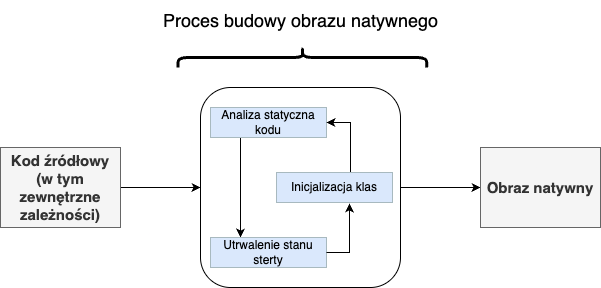
\includegraphics[width=0.95\textwidth]{charts/graalvm-build-process.drawio.png}
    \caption{Uproszczony proces budowy obrazu natywnego GraalVM [źródło:~opracowanie~własne]}
    \label{fig:graalvm_build_process}
\end{figure}

Kolejnym aspektem, który może negatywnie wpłynąć na rozwój oprogramowania przy użyciu GraalVM, jest czasochłonność procesu kompilacji.
Generowanie w pełni zoptymalizowanego obrazu natywnego jest operacją bardziej złożoną niż standardowa kompilacja kodu Javy do postaci bajtowej.
W praktyce oznacza to, że proces budowania artefaktu dla funkcji AWS Lambda może trwać odczuwalnie dłużej.
Może mieć to znaczący wpływ na rozwój oprogramowania, szczególnie w przypadku częstych iteracji i tworzenia nowych wersji funkcji.
Dłuższy czas kompilacji może także wpłynąć na ogólną efektywność procesów ciągłej integracji i ciągłego dostarczania (ang. CI/CD).

Jednym z sposobów poprawy doświadczeń programistów przy pracy z GraalVM, jest użycie odpowiednich frameworków.
Jednym z nich jest Quarkus \cite{9245290}, który został zaprojektowany z myślą o środowiskach chmurowych.
Kluczową cechą Quarkusa jest przeniesienie jak największej liczby operacji inicjalizacyjnych i konfiguracyjnych na etap budowania aplikacji.
Obejmuje to między innymi wstrzykiwanie zależności, przetwarzanie adnotacji oraz konfigurację rozszerzeń. 
Dzięki temu, w czasie budowania obrazu natywnego, Quarkus jest w stanie przeprowadzić szczegółową analizę aplikacji.
Poprzez użycie odpowiednich annotacji pozwala on na oznaczenie klas niezbędnych dla mechanizmów refleksji czy proxy \cite{quarkus-docs}.
Dzięki temu jest on w stanie automatycznie wygenerować niezbędne metadane dla klas.
Dane te następnie pozwalają na użycie wspomnianych mechanizmów w GraalVM.
Innymi, konkurencyjnymi do Quarkusa frameworkami, które oferują wsparcie dla obrazów natywnych są Helidon i Micronaut \cite{9245290}.
Ich popularność wskazuje na wysokie zainteresowanie takimi technologiami w społeczności programistów Java, dlatego jest to interesujący kierunek rozwoju dla funkcji AWS Lambda.

\section{Kotlin}\label{chapter:kotlin_multiplatform}

W ramach systematycznego przeglądu literatury (przedstawionego w Rozdziale \ref{chapter:przeglad_literatury}) zauważono, że aktualne badania skupiają się wyłącznie na języku Java.
Pomijają one jednak inne języki z ekosystemu Java, także oparte o maszynę wirtualną Java (ang. JVM).
Tymczasem na popularności zyskują alternatywne języki ekosystemu Javy.
Wśród nich na szczególną uwagę zasługuje Kotlin, rozwijany przez firmę JetBrains.
Jest on oficjalnie wspierany przez Google jako język programowania dla platformy Android, co wskazuje na jego solidne zastosowanie w tych systemach.
Coraz większe uznanie zyskuje także jako działający po stronie serwera. 
Dlatego język ten jest interesującym obszarem badań w kontekście AWS Lambda.
W tym rozdziale przedstawiony zostanie język programowania Kotlin, w tym jego zastosowanie w kontekście funkcji AWS Lambda.

Jednym z kluczowych czynników, które zwiększają popularność Kotlina, jest jego łatwa nauka przez programistów Javy.
Dodatkowo, istnieje możliwość łatwej intergracji kodu napisanego w Kotlinie z istniejącym oprogramowaniem Java \cite{kotlinlangKotlinDocs}.
Te cechy czynią go interesującym kandydatem do analizy w kontekście optymalizacji wydajności rozwiązań dla usługi AWS Lambda. 
Dla zespołów programistycznych może stanowić on wartościowe rozszerzenie dotychczasowych możliwości. 
Kotlin oferuje bowiem alternatywę lub uzupełnienie dla tradycyjnie stosowanej Javy.

Kwestia wydajności Kotlina w porównaniu do Javy jest przedmiotem dyskusji. 
Jednak badania dotyczą najczęściej ich zastosowań w kontekście aplikacji mobilnych.
Gajek i inni autorzy \cite{Gajek_Plechawska-Wójcik_2024} przeanalizowali wydajność obu języków, poprzez użycie gry mobilnej uruchomionej na systemie Android.
Wykazali oni, że w testowanym scenariuszu Java osiągnęła nieznacznie lepszą wydajność pod względem zużycia zasobów CPU i RAM.
Było to jednak zastosowanie mobilne, a same różnice nie były znaczne.
Należy jednak podkreślić, że warunki mobilne mogą być inne niż w systemach działających w usłudze AWS Lambda.
Sam język Kotlin posiada mechanizmy, które mogą pozytywnie wpłynąć na wydajność.

Funkcje inline (ang. inline functions) w Kotlinie mogą przyczynić się do redukcji narzutu wydajności podczas wywołań funkcji.
Mechanizm ten polega na wstawieniu kodu ciała funkcji bezpośrednio w miejsce jej wywołania \cite{kotlinlangKotlinDocs}.
Jest to wykonywane w momencie kompilacji, a programista może określić, które funkcje powinny być w ten sposób optymalizowane.
Eliminuje to koszt ich wywołania, co jest szczególnie przydatne w przypadku małych, często używanych funkcji.
Dodatkowo, język pozwala na przekazywanie funkcji jako parametrów, na przykład w kolekcjach i metodach jak filtrowanie.
W tych sytuacjach użycie funkcji inline może znacząco zmniejszyć liczbę operacji.
Pozytywny wpływ mechanizmu inline został przedstawiony przez Bergstrom i innych autorów \cite{DBLP:journals/corr/BergstromFRS13}, gdzie jego użycie zmniejszyło czas wykonywania programów nawet do 8\%.

Innym istotnym elementem Kotlina wspierającym wydajność są korutyny (ang. coroutines).
Mogą być one użyteczne zwłaszcza w kontekście operacji wejścia-wyjścia (I/O).
Systemy oparte o usługę AWS Lambda często integrowane są z zewnętrznymi serwisami (co zostało zauważone w ramach przeglądu literatury w Rozdziale \ref{chapter:przeglad_literatury}).
Wymaga to komunikacji opartej o operacje sieciowe.
Tradycyjne podejście oparte na wątkach może konsumować dużą ilość zasobów serwera i prowadzić do blokowania wykonania.
Korutyny pozwalają na pisanie asynchronicznego, nieblokującego kodu w sposób bardziej sekwencyjny i czytelny \cite{kotlinlangKotlinDocs}.
Na lepszą wydajność korutyn w porównaniu z tradycyjnymi wątkami wskazali Beronić i inni autorzy \cite{9803765}.

Implementacja mechanizmów poprawiających wydajność w języku programowania, pozwala następnie na ich użycie w bibliotekach, które są wykorzystywane przez programistów.
Język Kotlin oferuje ciekawy ekosystem bibliotek, przeznaczonych na przykład do tworzenia aplikacji działających po stronie serwera.
Są to biblioteki jak http4k czy ktor.
Ktor to framework zaprojektowany do budowy asynchronicznych aplikacji serwerowych i klienckich, rozwijany przez firmę JetBrains.
Jest on oparty w pełni o język Kotlin, a jego kluczową cechą jest natywne wsparcie dla korutyn.
Z kolei http4k kładzie nacisk na prostotę i minimalizm.
Architektura http4k opiera się na koncepcji funkcji jako podstawowych bloków aplikacji \cite{http4kCoreDocs}, co naturalnie współgra z modelem serverless i AWS Lambda.
Samo narzędzie rezyguje z mechanizmów refleksji \cite{http4kCoreDocs}, co może mieć pozytywny wpływ na wydajność.

Rosnące znaczenie Kotlin dostrzega także Amazon Web Service, które oferuje bibliotekę AWS SDK dla Kotlina \cite{awsSDKForKotlinDeveloperGuide}.
Jej celem jest zapewnienie programistom możliwości interakcji z usługami AWS w sposób naturalny dla tego języka.
SDK ten został zaprojektowany od podstaw z myślą o Kotlinie, co przejawia się między innymi w wykorzystaniu korutyn do obsługi operacji asynchronicznych.

Duży wpływ na wydajność funkcji AWS Lambda ma wybrany język programowania \cite{8605773}\cite{Cordingly2020704}.
Wynika to na przykład z różnych przypadków biznesowych i operacji, które muszą wykonywać.
Mimo to, często muszą one dzielić wspólny kod \cite{8116416}, co wskazuje na potrzebę wykorzystania mechanizmów, które to umożliwą.
Z tego powodu bardzo interesującą dla AWS Lambda i jej wydajności, może okazać się inicjatywa Kotlin Multiplatform.
KMP (Kotlin Multiplatform) to projekt, który powstał w szczególności dla aplikacji mobilnych.
Pozwala on na kompilację lub translację tego samego kodu Kotlin do użycia na różnych platformach.
Mogą to być na przykład Android, iOS, aplikacje desktopowe (JVM) lub webowe (JavaScript, Web Assembly) \cite{kotlinlangKotlinDocs}.
Oferuje to możliwość dzielenia kodu (np. logiki biznesowej) pomiędzy różnymi platformami, jednak przy możliwości zachowania natywnych komponentów widoku.

Mimo głównego przypadku użycia jakim są aplikacje klienckie, Kotlin Multiplatform może być obiecującym rozwiązaniem dla AWS Lambda.
Po pierwsze oferuje on możliwość translacji kodu Kotlin do JavaScript oraz kompilację do natywnych plików binarnych (opcje te zostaną przedstawione jako osobne metody w kolejnych rozdziałach).
Pozwala to na ominięcie różnych niedogodności wynikających z użycia maszyny wirtualnej Javy.
Jednak zachowane są przy tym zalety języka oraz wspiera to użycie już istniejących umiejętności programistów języków rodziny JVM.
Po drugie, kod w KMP może być dzielony pomiędzy platformami.
Umożliwia to bardzo elastyczny wybór środowiska uruchomieniowego AWS Lambda w ramach pojedynczego systemu.
Jednocześnie, część kodu może być współdzielona między wszystkie funkcje niezależnie od wybranej platformy.
Może to na przykład oznaczać, że klasy implementujące pewne struktury oraz zasady wynikające z reguł biznesowych, będą mogły być używane przez funkcje działające zarówno poprzez JavaScript, JVM, jak i natywne pliki binarne. 

Jednym z czynników, które mogą być modyfikowane już podczas działania usług AWS Lambda jest pamięć.
Jej rozmiar może być dostosowywany w zależności od wydajności monitorowanej funkcji.
Użycie Kotlin Multiplatform pozwala na rozszerzenie tej metody.
W zależności od obserwowanych parametrów (jak czas odpowiedzi lub opóźnienia zimnych startów) możliwe jest ponowne wykorzystanie tego samego kodu i budowa funkcji działającej na innej platformie.
Przykładowo, po wdrożeniu funkcji działającej z użyciem JVM, może pojawić się potrzeba redukcji czasu zimnych startów.
W takim wypadku Kotlin Multiplatform umożliwia translację kodu do JavaScript, który pozwoli na redukcję czasu inicjalizacji AWS Lambda.

Współdzielenie kodu pomiędzy platformami jest możliwe dzięki strukturze, którą oferuje Kotlin Multiplatform.
Została ona opisana przez firmę JetBrains w ramach dokumentacji KMP \cite{kotlinMultiplatformDev}.
Jej głównym elementem jest katalog ,,commonMain'', który jest współdzielony pomiędzy wszystkimi platformami.
Kompilator używa kodu współdzielonego jako dane wejściowe, aby w rezultacie utworzyć zestaw plików binarnych specyficznych dla danej platformy.
Mogą to być na przykład pliki .class dla maszyny wirtualnej Javy, czy natywne pliki wykonywalne (np. dla platformy Linux).

\begin{figure}[h]
    \centering
    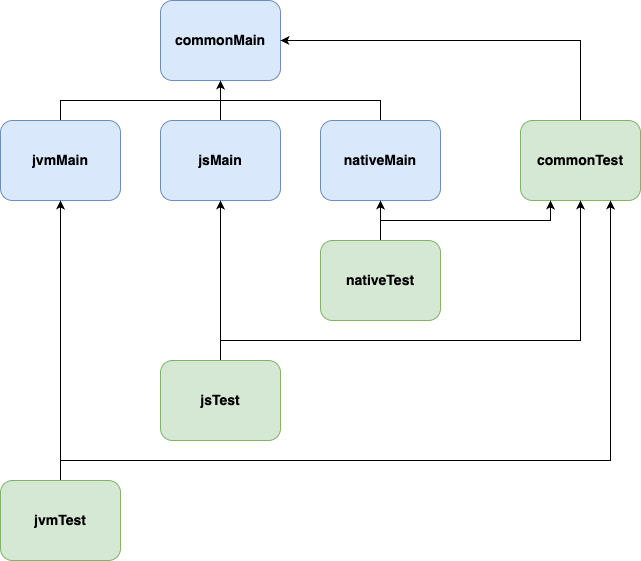
\includegraphics[width=0.95\textwidth]{charts/kmp-structure.drawio.png}
    \caption{Przykładowa struktura pojektu Kotlin Multiplatform [źródło:~opracowanie~własne]}
    \label{fig:kmp_project_structure}
\end{figure}

Następnie programista może utworzyć kolejne katalogi, które będą zawierać kod specyficzny dla docelowych platform.
Przykładowa struktura została przedstawiona na Rysunku \ref{fig:kmp_project_structure}, gdzie katalog commonMain jest wspóldzielony między JVM (jvmMain), JavaScript (jsMain) oraz platformy natywne (nativeMain).
Docelowe platformy (ang. targets) są deklarowane w konfiguracji Gradle \cite{kotlinMultiplatformDev}, a kod współdzielony jest przygotowywany wyłącznie dla nich.
Katalogi dla docelowych platform są wymagane, gdyż Kotlin nie zezwala na użycie specyficznych elementów danej platformy w katalogu współdzielonym.
Przykładem takiego elementu może być klasa ,,java.io.File'', która jest dostępna wyłącznie dla maszyny wirtualnej Javy.
Jej użycie w katalogu commonMain spowoduje błąd kompilacji.

Kotlin Multiplatform zawiera także integracje z testami oprogramowania.
Jest to szczególnie ważne dla tworzenia oprogramowania z wykorzystaniem AWS Lambda, gdzie testowanie może być skomplikowane (co było jednym z wniosków przeglądu literatury w Rozdziale \ref{chapter:przeglad_literatury}).
Testy dla kodu współdzielonego powinny być zapisane w katalogu ,,commonTest'', gdzie programista może użyć biblioteki kotlin.test \cite{kotlinMultiplatformDev}.
Następnie testy są uruchamiane dla każdej docelowej platformy.
Programista może także tworzyć przypadki testowe dla konkretnych platform, z użyciem technologii przez nie oferowanych.
Następuje tutaj analogiczne współdzielenie kodu jak dla katalogów ,,main'', co zostało także zawarte w Rysunku \ref{fig:kmp_project_structure}.

Specyficzne cechy Kotlina jak funkcjonalności języka, biblioteki czy projekt Kotlin Multiplatform mogą zapewnić znaczne wzrosty wydajności funkcji AWS Lambda.
Mimo, że Kotlin jest językiem wywodzącym się z Javy oferuje już możliwości, które mogą pozwolić na osiągnięcie niższych czasów odpowiedzi.
Dodatkowo, sposoby te nie zostały jeszcze przebadane. 
Dlatego Kotlin to obszar, który zasługuje na zawarcie go w badanich na temat wydajności AWS Lambda.

\section{Kotlin/JS}\label{chapter:kotlin_js}

\section{Kotlin/Native}\label{chapter:kotlin_native}

Bardzo skuteczną metodą optymalizacji wydajności może być rezygnacja z zarządzanych środowisk uruchomieniowych jak JVM.
Jedną z metod jest kompilacja do kodu natywnego, który uruchamiany jest bezpośrednio na systemie operacyjnym poza maszyną wirtualną.
Kotlin/Native oferuje zaawansową kompilację kodu Kotlin, który następnie może zostać uruchomiony w AWS Lambda z użyciem Amazon Linux.
W ramach rozdziału opisano sposób działania Kotlin/Native, jego możliwości i cechy, które mogą negatywnie wpłynąć na rozwój oprogramowania bezserwerowego.

Kluczowym elementami Kotlin/Native są kompilator oparty o LLVM oraz natywne implementacje bibliotek standardowych Kotlina \cite{kotlinlangKotlinDocs}.
Jak opisują Lattner i Adve \cite{1281665}, LLVM to framework kompilatora zaprojektowany do wspierania ciągłej i transparentnej analizy oraz transformacji programów.
Definiuje on wspólną, niskopoziomową reprezentację kodu w formie SSA (ang. Static Single Assignment) z systemem typów niezależnym od języka, co umożliwia implementację cech języków wysokiego poziomu. 
Głównym celem LLVM jest umożliwienie analizy i transformacji programu na różnych etapach jego życia, w tym w czasie kompilacji, linkowania, uruchomienia oraz w czasie bezczynności między uruchomieniami.
Jego użycie pozwala następnie na zbudowanie natywnych plików binarnych, które mogą zostać uruchomione bezpośrednio na docelowej platformie, dla której zostały skompilowane.
Wymaga to jednak dokładnego określenia systemu operacyjnego i architektury już w momencie kompilacji.

Kompilacja Kotlina do kodu natywnego otwiera przez KMP możliwość tworzenia samodzielnych programów wykonywalnych, które nie wymagają zewnętrznego środowiska uruchomieniowego.
Znajduje to zastosowanie w scenariuszach takich jak rozwój aplikacji mobilnych na platformę iOS, współdzielenie logiki biznesowej między różnymi platformami (np. Android i iOS) czy budowa narzędzi konsolowych.
Dlatego ważnym aspektem Kotlin/Native jest współdziałanie z istniejącym kodem natywnym.
Pozwala to na bezpośrednie wywoływanie funkcji z bibliotek napisanych w języku C, a na platformach firmy Apple również Objective-C \cite{kotlinlangKotlinDocs}.
Znacząco rozszerza to zakres dostępnych narzędzi i bibliotek, które mogą zostać użyte przez programistów.

Kotlin/Native oferuje wiele różnych platform docelowych, rozszerzając tym samym zakres zastosowań języka Kotlin.
Wśród wspieranych systemów docelowych znajdują się platformy Apple (takie jak macOS, iOS, watchOS, tvOS), Android, a także systemy z rodziny Windows oraz Linux \cite{kotlinlangKotlinDocs}.
Szczególnie istotnie dla usługi AWS Lambda są jednak platformy linuxowe.
Są to linuxX64 oraz linuxArm64, które pozwalają na uruchomienie kodu z użyciem odpowiednio architektur x86 oraz ARM.
Pozwala to następnie na ich bezpośrednie użycie w AWS Lambda, działającej bezpośrednio w systemie Amazon Linux.
Dzięki temu możliwa jest poprawa wydajności, szczególnie w aspekcie zimnych startów, które są znacznym wyzwaniem dla funkcji opartych o JVM.

Istotnym elementen funkcji bezserwerowych jest zarządzanie pamięcią, która wpływa bezpośrednio na koszty.
W przypadku Kotlin/Native, ewolucja modelu zarządzania pamięcią znacząco wpłynęła na jego użyteczność i możliwości optymalizacyjne.
Początkowa technologia ta opierała się na restrykcyjnym modelu z izolacją obiektów między wątkami \cite{kotlinlangKotlinDocs}.
Powodowało to skomplikowane zarządzanie stanem w operacjach współbieżnych.
Aktualnie, Kotlin/Native implementuje nowy menedżer pamięci.
Wprowadza on automatyczne zarządzanie pamięcią poprzez współbieżny, nieblokujący moduł zbierania śmieci (ang. garbage collector) \cite{kotlinlangKotlinDocs}.
Znacząco upraszcza to programowanie współbieżne, które teraz nie wymaga ręcznego zarządzania obiektami.
Mechanizm ten wprowadza intuicyjne współdzielenie stanu, które jest analogiczne do środowiska JVM, jednak bez konieczności kosztownej obsługi maszyny wirtualnej Java.

Mimo potencjalnych zysków w ramach wydajności, użycie Kotlin/Native może nieść utrudnienia w kontekście integracji z bibliotekami zewnętrznymi.
Język C nie jest oficjalnie wspierany jako język programowania AWS Lambda \cite{awsLambdaDeveloperGuide}, co wynika zapewne z jego niewielkiej popularności na tej platformie.
Współdziałanie z kodem natywnym w Kotlin/Native skupia się jednak na platformach klienckich, co nie musi być do końca użyteczne w zakresie AWS Lambda.
Amazon Web Services oferuje swoje SDK w języku C++, który nie jest jednak łatwo integrowalny z Kotlin/Native (w odróżnieniu od C i Objective-C).
Jest to ważny czynnik, który powinien być uwzględniony przez programistów projektujących aplikacje bezserwerowe.

% Plan
% 0. Wstęp

% 1. Jak to działa:
% - Opisać LLVM
% - Gdzie się głównie używa
% - Wspomnieć o interoperacyjności z C, Objective-C itp
% - Jakie platformy? (https://kotlinlang.org/docs/native-target-support.html#for-library-authors)

% 2. Zarządzanie pamięcią (https://kotlinlang.org/docs/native-memory-manager.html)

% 3. Wady - problem z dostępnością bibliotek
% - AWS SDK może poprzez C++ jednak może to wymagać większego nakładu pracy


\chapter{Wybrane metody optymalizacji}\label{chapter:wybrane_metody_optimalizacji}

% TODO: jakiś wstęp, typu jakich metod brakowało w przeglądzie. Podkreślić brak innych języków
\section{SnapStart}\label{chapter:snapstart}

Jednym z istotnych czynników wpływających na wydajność funkcji AWS Lambda implementowanych w ekosystemie Java jest zjawisko tzw. zimnego startu.
Wynika on z cyklu życia funkcji i etapu inicjalizacji (co zostało opisane w Rozdziale \ref{chapter:aws_lambda}).
W etap ten wchodzą procesy takie jak inicjalizacja maszyny wirtualnej Java czy uruchomienie statycznego kodu inicjującego \cite{awsLambdaDocs}.
W przypadku Javy zajmuje to więcej czasu niż dla innych języków (jak Python), co wydłuża zimne starty \cite{8605773}.
Znacząco oddziałuje to na wydajność funkcji, a może być szczególnie dotkliwe dla serwisów o niewielkiej aktywności.
W odpowiedzi na potrzebę minimalizacji tych negatywnych skutków Amazon Web Services wprowadziło mechanizm znany jako AWS Lambda SnapStart.
W ramach podrozdziału podjęto analizę tego rozwiązania w kontekście jego działania, zalet oraz ograniczeń. 

Mechanizm SnapStart istotnie modyfikuje tradycyjny cykl życia funkcji AWS Lambda.
Zasadnicza różnica polega na przeniesieniu kosztownego etapu inicjalizacji z momentu pierwszego wywołania funkcji na etap jej publikacji \cite{amazonSnapstartDeveloperGUide}.
Oznacza to, że inicjalizacja funkcji nie jest wykonywana w momencie zapytania użytkownika (co wywołuje zimny start), lecz w momencie wgrania nowej wersji funkcji (oraz kodu) przez programistę.
Inicjalizacja ta zawiera najdłuższe operacje dla rozwiązań Java jak utworzenie maszyny wirtualnej, załadowanie klas, czy wykonanie kodu inicjalizującego.
Następnie, tworzona jest zaszyfrowana ,,migawka'' (ang. snapshot) stanu pamięci i dysku w pełni gotowego środowiska wykonawczego.
Gdy funkcja jest następnie wywoływana po raz pierwszy, nie zachodzi już standardowy zimny start.
Zamiast tego środowisko jest odtwarzane z utworzonej migawki, co zostało przedstawione na Rysunku \ref{fig:aws_lambda_snapstart_process}.
Według dostawcy AWS metoda ta w optymalnych scenariuszach zmniejsza opóźnienie z kilku sekund do mniej niż sekundy \cite{amazonSnapstartDeveloperGUide}. 

\begin{figure}[h]
    \centering
    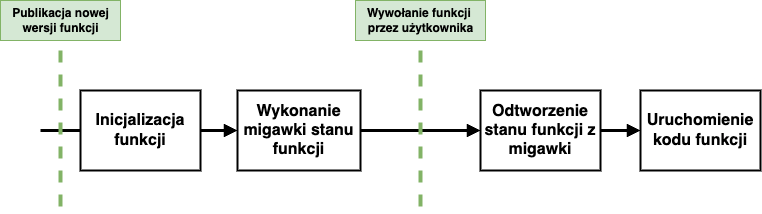
\includegraphics[width=0.95\textwidth]{charts/snapstart.png}
    \caption{Proces uruchomienia AWS Lambda z użyciem metody SnapStart [źródło:~opracowanie~własne]}
    \label{fig:aws_lambda_snapstart_process}
\end{figure}

Działanie tej metody jest technicznie możliwe dzięki użyciu środowiska wirtualizacji przez AWS Lambda.
Jak opisują Agache i inni autorzy \cite{246288} usługa Lambda do izolacji poszczególnych funkcji wykorzystuje dedykowane maszyny wirtualne typu microVM.
Są one zarządzane przez lekki monitor maszyn wirtualnych (ang. VMM) o nazwie Firecracker.
Posiada on cechy, które były kluczowe w minimalizacji problemu zimnego startu.
Po pierwsze, celowo rezygnuje on z emulacji zbędnych urządzeń (jak emulacja systemu BIOS czy rozbudowanych kontrolerów PCI) \cite{246288}.
Zmniejsza to złożoność i rozmiar stanu każdej maszyny wirtualnej. 
Dzięki temu wykonanie i odtworzenie migawki jest łatwiejsze.
Po drugie, Firecracker jest w pełni kontrolowany przez interfejs REST API \cite{246288}.
Umożliwia to precyzyjne zarządzanie całym cyklem życia każdej maszyny wirtualnej, włączając w to jej konfigurację, uruchomienie oraz zatrzymanie.
Pozwala to na określenie fazy inicjalizacji funkcji oraz wykonanie migawki w odpowiednim momencie.
Istotna jest również zapewniona przez Firecracker izolacja \cite{246288}, co gwarantuje bezpieczeństwo tworzenia i odtwarzania migawek.

Samo użycie metody SnapStart jest bardzo proste i nie wymaga od programisty dużego nakładu pracy.
Włączenie rozwiązania wymaga jedynie ustawienia odpowiedniej opcji podczas konfiguracji funkcji \cite{amazonSnapstartDeveloperGUide}.
Nie oznacza to jednak, że SnapStart jest odpowiedni dla wszystkich funkcji.
AWS podkreśla dwa typy aplikacji, które znacząco zyskają poprzez użycie SnapStart \cite{amazonSnapstartDeveloperGUide}.
Są nimi wrażliwe na opóźnienia interfejsy API i potoki przetwarzania danych.
Dodatkowo, metoda ta niesie za sobą pewne ograniczenia, które muszą zostać uwzględnione przed jej wdrożeniem.

Pierwszym aspektem jest kwestia unikalności stanu w funkcjach wykorzystujących SnapStart.
Jak analizują Brooker i inni autorzy \cite{brooker2021restoringuniquenessmicrovmsnapshots}, klonowanie migawek wprowadza fundamentalne wyzwanie związane z przywróceniem unikalności maszyn wirtualnych, co jest niezbędne do poprawnego generowania unikalnych identyfikatorów czy sekretów kryptograficznych.
Migawka zainicjowanego środowiska wykonywana jest jednorazowo, a następnie używana podczas wielu wywołań funkcji.
Może to stanowić duże zagrożenie dla programisty AWS Lambda, gdy potrzebuje on generować unikalne wartości jak identyfikatory (np. UUID) czy jednorazowe tokeny.
Narusza to znacznie poprawność logiki aplikacji oraz jej bezpieczeństwo.
Jedną z metod naprawy tego problemu jest generowanie wartości losowych wyłącznie w metodzie wywołującej funkcje (zamiast w bloku statycznym kodu) \cite{amazonSnapstartDeveloperGUide}.
Dodatkowo, ewentualne problemy z unikalnością funkcji SnapStart mogą zostać wykryte poprzez oprogramowanie SpotBugs \cite{SpotBugsProject}.
Narzędzie wykonuje statyczną analizę kodu, walidując go poprzez reguły zapewnione przez AWS.
Pozwala to programiście wykryć, a następnie naprawić fragmenty kodu powodujące problem z unikalnością.

Kolejnym istotnym wyzwaniem podczas rozwoju aplikacji z technologią SnapStart jest zarządzanie połączeniami sieciowymi \cite{amazonSnapstartDeveloperGUide}.
Połączenia nawiązane z zewnętrznymi usługami są standardową praktyką podczas tworzenia aplikacji AWS Lambda \cite{eismann2021reviewserverlessusecases}\cite{Ivanov_Petrova_2024}.
Problematyczne stają się jednak te połączenia sieciowe, które nawiązano podczas inicjalizacji funkcji. 
Ponieważ inicjalizacja odbywa się przed faktycznym przetworzeniem żądania użytkownika, upływający czas może sprawić, że w momencie odtworzenia funkcji połączenia te nie będą już aktywne.
Praktyką zalecaną przez AWS jest ponowne nawiązywanie lub dokładna walidacja istniejących połączeń \cite{amazonSnapstartDeveloperGUide}.
Powinno to być wykonane bezpośrednio w metodzie wywołującej funkcje lub z wykorzystaniem metody ,,afterRestore''.
Metoda ta jest wywoływana bezpośrednio po odtworzeniu migawki stanu funkcji.

Strategicznym czynnikiem usług bezserwerowych są koszty, zatem powinny być one uwzględnione także przed użyciem SnapStart.
Zgodnie z dokumentacją Amazon Web Services \cite{amazonSnapstartDeveloperGUide}, użycie SnapStart dla środowisk uruchomieniowych Java nie wiążą się z dodatkowymi kosztami.
Koszt wykonania funkcji z włączonym SnapStart nadal bazuje na standardowych rozliczeniach.
Składa się na niego liczba przetworzonych żądań oraz łączny czas trwania wykonań.

Podsumowując, mechanizm SnapStart stanowi prostą w aktywacji metodę redukcji czasu zimnych startów.
Sam mechanizm opiera się na wcześniejszym wykonaniu fazy inicjacji funkcji, a następnie wykonania migawki stanu.
W momencie wywołania funkcji stan ten może zostać odtworzony.
Znaczącą korzyścią metody jest brak dodatkowych kosztów.
Wiąże się ona jednak z istotnymi utrudnieniami (jak zarządzanie połączeniami sieciowymi i problem z unikalnością stanu).
Powinny być one uwzględnione przez programistę przed użyciem narzędzia.
\section{GraalVM}\label{chapter:graalvm}

Ważnym obszarem badań nad optymalizacją Javy i jej użycia w AWS Lambda, są technologie pozwalające na zmianę sposobu kompilacji i uruchamiana aplikacji.
Jedną z technologii, które zyskusje na popularności w tym zakresie, jest GraalVM.
Jest to możliwe m.in. dzięki użyciu kompilatora JIT (ang. Just-In-Time) w połączeniu z kompilacją AOT (ang. Ahead-Of-Time) \cite{8756917}.
GraalVM oferuje zaawansowaną architekturę pozwalającą na kompilację i uruchomienie aplikacji w postaci obrazów natywnych.
Stanowi to alternatywę dla klasycznej maszyny wirtualnej Javy, a dodatkowo skupia się na jej wydajności.
Poniższy podrozdział poświęcono analizie działania omawianego rozwiązania, jego zalet i słabych stron.

Kluczowym mechanizmem GraalVM jest kompilacja AOT (ang. Ahead-Of-Time) do postaci tzw. obrazów natywnych (ang. native images) \cite{8756917}.
Ma to bezpośredni wpływ na wydajność działania aplikacji.
W modelu tradycyjnym, kod bajtowy Java jest interpretowany i kompilowany dynamicznie przez maszynę wirtualną w trakcie działania aplikacji.
Podejście AOT przenosi znaczną część z tych operacji na etap budowania artefaktu. 
Istotnym elementem tego procesu jest agresywna, statyczna analiza kodu \cite{9245290}, w celu identyfikacji osiągalnych w trakcie działania części.
Pozwala to na odrzucenie nieużywanych fragmentów kodu (np. z używanych bibliotek), co pozwala na zmniejszenie wielkości obrazu natywnego.
Aspekt ten może być kluczowy w kontekście AWS Lambda, ze względu na wpływ wielkości artefaktu na wydajność \cite{8116416}.
Po analizie kodu, dokonywana jest inicjalizacja klas, a stan aplikacji, w tym częściowo zainicjalizowana sterta, jest utrwalany.
W celu lepszej optymalizacji, operacje te są powtarzane, co zostało przedstawione na Rysunku \ref{fig:graalvm_build_process}.

Jako wynik kompilacji powstaje samodzielny, zoptymalizowany plik binarny.
Nie wymaga on do uruchomienia pełnej maszyny wirtualnej Java, a jedynie minimalnego środowiska wykonawczego dostarczanego przez SubstrateVM, będącego częścią GraalVM \cite{8756917}.
Różnica ta ma fundamentalne znaczenie w kontekście wydajności AWS Lambda.
Eliminowana jest konieczność wykonywania czasochłonnych operacji typowych dla startu tradycyjnej maszyny wirtualnej Java, takich jak ładowanie klas czy jej inicjalizacja.
Wszystkie te zadania zostały już wykonane wcześniej, w procesie budowy obrazu natywnego.
Dzięki temu tworzona przez programistę funkcja AWS Lambda nie będzie operować w zarządzanym środowisku Java.
Zamiast tego, usługi muszą opierać się o niestandardowe środowiska wykonawcze, oferujące wyłącznie system operacyjny (Amazon Linux 2023 lub Amazon Linux 2) \cite{awsLambdaDeveloperGuide}.
Ich użycie pozwala także na realizację drugiej zalety GraalVM, czyli redukcji zapotrzebowania na pamięć operacyjną \cite{9245290}.

Pomimo pozytywnego wpływu na wydajność, zastosowanie kompilacji AOT w GraalVM wiąże się także z ograniczeniami.
Jednym z nich jest obsługa dynamicznych cech Javy, takich jak refleksja (ang. reflection), dynamiczne proxy, serializacja czy natywny interfejs Java (JNI)
Wynika to z faktu użycia agresywnej statycznej analizy kodu.
Napotyka ona trudności w przewidzeniu wszystkich dynamicznie ładowanych klas, pól i metod, które nie są jawnie osiągalne w kodzie źródłowym.
Problem ten wymaga użycia dodatkowych mechanizmów GraalVM \cite{graalvm-reflection-jdk21}.
Polegają one na przygotowaniu dodatkowych metadanych dla klas, co wymaga jednak dodatkowej obsługi.

\begin{figure}
    \centering
    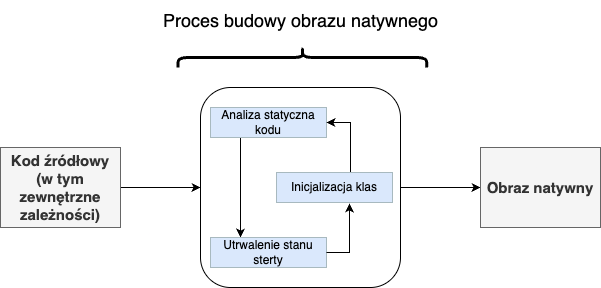
\includegraphics[width=0.95\textwidth]{charts/graalvm-build-process.drawio.png}
    \caption{Uproszczony proces budowy obrazu natywnego GraalVM [źródło:~opracowanie~własne]}
    \label{fig:graalvm_build_process}
\end{figure}

Kolejnym aspektem, który może negatywnie wpłynąć na rozwój oprogramowania przy użyciu GraalVM, jest czasochłonność procesu kompilacji.
Generowanie w pełni zoptymalizowanego obrazu natywnego jest operacją bardziej złożoną niż standardowa kompilacja kodu Javy do postaci bajtowej.
W praktyce oznacza to, że proces budowania artefaktu dla funkcji AWS Lambda może trwać odczuwalnie dłużej.
Może mieć to znaczący wpływ na rozwój oprogramowania, szczególnie w przypadku częstych iteracji i tworzenia nowych wersji funkcji.
Dłuższy czas kompilacji może także wpłynąć na ogólną efektywność procesów ciągłej integracji i ciągłego dostarczania (ang. CI/CD).

Jednym z sposobów poprawy doświadczeń programistów przy pracy z GraalVM, jest użycie odpowiednich frameworków.
Jednym z nich jest Quarkus \cite{9245290}, który został zaprojektowany z myślą o środowiskach chmurowych.
Kluczową cechą Quarkusa jest przeniesienie jak największej liczby operacji inicjalizacyjnych i konfiguracyjnych na etap budowania aplikacji.
Obejmuje to między innymi wstrzykiwanie zależności, przetwarzanie adnotacji oraz konfigurację rozszerzeń. 
Dzięki temu, w czasie budowania obrazu natywnego, Quarkus jest w stanie przeprowadzić szczegółową analizę aplikacji.
Poprzez użycie odpowiednich annotacji pozwala on na oznaczenie klas niezbędnych dla mechanizmów refleksji czy proxy \cite{quarkus-docs}.
Dzięki temu jest on w stanie automatycznie wygenerować niezbędne metadane dla klas.
Dane te następnie pozwalają na użycie wspomnianych mechanizmów w GraalVM.
Innymi, konkurencyjnymi do Quarkusa frameworkami, które oferują wsparcie dla obrazów natywnych są Helidon i Micronaut \cite{9245290}.
Ich popularność wskazuje na wysokie zainteresowanie takimi technologiami w społeczności programistów Java, dlatego jest to interesujący kierunek rozwoju dla funkcji AWS Lambda.

\section{Kotlin}\label{chapter:kotlin_multiplatform}

W ramach systematycznego przeglądu literatury (przedstawionego w Rozdziale \ref{chapter:przeglad_literatury}) zauważono, że aktualne badania skupiają się wyłącznie na języku Java.
Pomijają one jednak inne języki z ekosystemu Java, także oparte o maszynę wirtualną Java (ang. JVM).
Tymczasem na popularności zyskują alternatywne języki ekosystemu Javy.
Wśród nich na szczególną uwagę zasługuje Kotlin, rozwijany przez firmę JetBrains.
Jest on oficjalnie wspierany przez Google jako język programowania dla platformy Android, co wskazuje na jego solidne zastosowanie w tych systemach.
Coraz większe uznanie zyskuje także jako działający po stronie serwera. 
Dlatego język ten jest interesującym obszarem badań w kontekście AWS Lambda.
W tym rozdziale przedstawiony zostanie język programowania Kotlin, w tym jego zastosowanie w kontekście funkcji AWS Lambda.

Jednym z kluczowych czynników, które zwiększają popularność Kotlina, jest jego łatwa nauka przez programistów Javy.
Dodatkowo, istnieje możliwość łatwej intergracji kodu napisanego w Kotlinie z istniejącym oprogramowaniem Java \cite{kotlinlangKotlinDocs}.
Te cechy czynią go interesującym kandydatem do analizy w kontekście optymalizacji wydajności rozwiązań dla usługi AWS Lambda. 
Dla zespołów programistycznych może stanowić on wartościowe rozszerzenie dotychczasowych możliwości. 
Kotlin oferuje bowiem alternatywę lub uzupełnienie dla tradycyjnie stosowanej Javy.

Kwestia wydajności Kotlina w porównaniu do Javy jest przedmiotem dyskusji. 
Jednak badania dotyczą najczęściej ich zastosowań w kontekście aplikacji mobilnych.
Gajek i inni autorzy \cite{Gajek_Plechawska-Wójcik_2024} przeanalizowali wydajność obu języków, poprzez użycie gry mobilnej uruchomionej na systemie Android.
Wykazali oni, że w testowanym scenariuszu Java osiągnęła nieznacznie lepszą wydajność pod względem zużycia zasobów CPU i RAM.
Było to jednak zastosowanie mobilne, a same różnice nie były znaczne.
Należy jednak podkreślić, że warunki mobilne mogą być inne niż w systemach działających w usłudze AWS Lambda.
Sam język Kotlin posiada mechanizmy, które mogą pozytywnie wpłynąć na wydajność.

Funkcje inline (ang. inline functions) w Kotlinie mogą przyczynić się do redukcji narzutu wydajności podczas wywołań funkcji.
Mechanizm ten polega na wstawieniu kodu ciała funkcji bezpośrednio w miejsce jej wywołania \cite{kotlinlangKotlinDocs}.
Jest to wykonywane w momencie kompilacji, a programista może określić, które funkcje powinny być w ten sposób optymalizowane.
Eliminuje to koszt ich wywołania, co jest szczególnie przydatne w przypadku małych, często używanych funkcji.
Dodatkowo, język pozwala na przekazywanie funkcji jako parametrów, na przykład w kolekcjach i metodach jak filtrowanie.
W tych sytuacjach użycie funkcji inline może znacząco zmniejszyć liczbę operacji.
Pozytywny wpływ mechanizmu inline został przedstawiony przez Bergstrom i innych autorów \cite{DBLP:journals/corr/BergstromFRS13}, gdzie jego użycie zmniejszyło czas wykonywania programów nawet do 8\%.

Innym istotnym elementem Kotlina wspierającym wydajność są korutyny (ang. coroutines).
Mogą być one użyteczne zwłaszcza w kontekście operacji wejścia-wyjścia (I/O).
Systemy oparte o usługę AWS Lambda często integrowane są z zewnętrznymi serwisami (co zostało zauważone w ramach przeglądu literatury w Rozdziale \ref{chapter:przeglad_literatury}).
Wymaga to komunikacji opartej o operacje sieciowe.
Tradycyjne podejście oparte na wątkach może konsumować dużą ilość zasobów serwera i prowadzić do blokowania wykonania.
Korutyny pozwalają na pisanie asynchronicznego, nieblokującego kodu w sposób bardziej sekwencyjny i czytelny \cite{kotlinlangKotlinDocs}.
Na lepszą wydajność korutyn w porównaniu z tradycyjnymi wątkami wskazali Beronić i inni autorzy \cite{9803765}.

Implementacja mechanizmów poprawiających wydajność w języku programowania, pozwala następnie na ich użycie w bibliotekach, które są wykorzystywane przez programistów.
Język Kotlin oferuje ciekawy ekosystem bibliotek, przeznaczonych na przykład do tworzenia aplikacji działających po stronie serwera.
Są to biblioteki jak http4k czy ktor.
Ktor to framework zaprojektowany do budowy asynchronicznych aplikacji serwerowych i klienckich, rozwijany przez firmę JetBrains.
Jest on oparty w pełni o język Kotlin, a jego kluczową cechą jest natywne wsparcie dla korutyn.
Z kolei http4k kładzie nacisk na prostotę i minimalizm.
Architektura http4k opiera się na koncepcji funkcji jako podstawowych bloków aplikacji \cite{http4kCoreDocs}, co naturalnie współgra z modelem serverless i AWS Lambda.
Samo narzędzie rezyguje z mechanizmów refleksji \cite{http4kCoreDocs}, co może mieć pozytywny wpływ na wydajność.

Rosnące znaczenie Kotlin dostrzega także Amazon Web Service, które oferuje bibliotekę AWS SDK dla Kotlina \cite{awsSDKForKotlinDeveloperGuide}.
Jej celem jest zapewnienie programistom możliwości interakcji z usługami AWS w sposób naturalny dla tego języka.
SDK ten został zaprojektowany od podstaw z myślą o Kotlinie, co przejawia się między innymi w wykorzystaniu korutyn do obsługi operacji asynchronicznych.

Duży wpływ na wydajność funkcji AWS Lambda ma wybrany język programowania \cite{8605773}\cite{Cordingly2020704}.
Wynika to na przykład z różnych przypadków biznesowych i operacji, które muszą wykonywać.
Mimo to, często muszą one dzielić wspólny kod \cite{8116416}, co wskazuje na potrzebę wykorzystania mechanizmów, które to umożliwą.
Z tego powodu bardzo interesującą dla AWS Lambda i jej wydajności, może okazać się inicjatywa Kotlin Multiplatform.
KMP (Kotlin Multiplatform) to projekt, który powstał w szczególności dla aplikacji mobilnych.
Pozwala on na kompilację lub translację tego samego kodu Kotlin do użycia na różnych platformach.
Mogą to być na przykład Android, iOS, aplikacje desktopowe (JVM) lub webowe (JavaScript, Web Assembly) \cite{kotlinlangKotlinDocs}.
Oferuje to możliwość dzielenia kodu (np. logiki biznesowej) pomiędzy różnymi platformami, jednak przy możliwości zachowania natywnych komponentów widoku.

Mimo głównego przypadku użycia jakim są aplikacje klienckie, Kotlin Multiplatform może być obiecującym rozwiązaniem dla AWS Lambda.
Po pierwsze oferuje on możliwość translacji kodu Kotlin do JavaScript oraz kompilację do natywnych plików binarnych (opcje te zostaną przedstawione jako osobne metody w kolejnych rozdziałach).
Pozwala to na ominięcie różnych niedogodności wynikających z użycia maszyny wirtualnej Javy.
Jednak zachowane są przy tym zalety języka oraz wspiera to użycie już istniejących umiejętności programistów języków rodziny JVM.
Po drugie, kod w KMP może być dzielony pomiędzy platformami.
Umożliwia to bardzo elastyczny wybór środowiska uruchomieniowego AWS Lambda w ramach pojedynczego systemu.
Jednocześnie, część kodu może być współdzielona między wszystkie funkcje niezależnie od wybranej platformy.
Może to na przykład oznaczać, że klasy implementujące pewne struktury oraz zasady wynikające z reguł biznesowych, będą mogły być używane przez funkcje działające zarówno poprzez JavaScript, JVM, jak i natywne pliki binarne. 

Jednym z czynników, które mogą być modyfikowane już podczas działania usług AWS Lambda jest pamięć.
Jej rozmiar może być dostosowywany w zależności od wydajności monitorowanej funkcji.
Użycie Kotlin Multiplatform pozwala na rozszerzenie tej metody.
W zależności od obserwowanych parametrów (jak czas odpowiedzi lub opóźnienia zimnych startów) możliwe jest ponowne wykorzystanie tego samego kodu i budowa funkcji działającej na innej platformie.
Przykładowo, po wdrożeniu funkcji działającej z użyciem JVM, może pojawić się potrzeba redukcji czasu zimnych startów.
W takim wypadku Kotlin Multiplatform umożliwia translację kodu do JavaScript, który pozwoli na redukcję czasu inicjalizacji AWS Lambda.

Współdzielenie kodu pomiędzy platformami jest możliwe dzięki strukturze, którą oferuje Kotlin Multiplatform.
Została ona opisana przez firmę JetBrains w ramach dokumentacji KMP \cite{kotlinMultiplatformDev}.
Jej głównym elementem jest katalog ,,commonMain'', który jest współdzielony pomiędzy wszystkimi platformami.
Kompilator używa kodu współdzielonego jako dane wejściowe, aby w rezultacie utworzyć zestaw plików binarnych specyficznych dla danej platformy.
Mogą to być na przykład pliki .class dla maszyny wirtualnej Javy, czy natywne pliki wykonywalne (np. dla platformy Linux).

\begin{figure}[h]
    \centering
    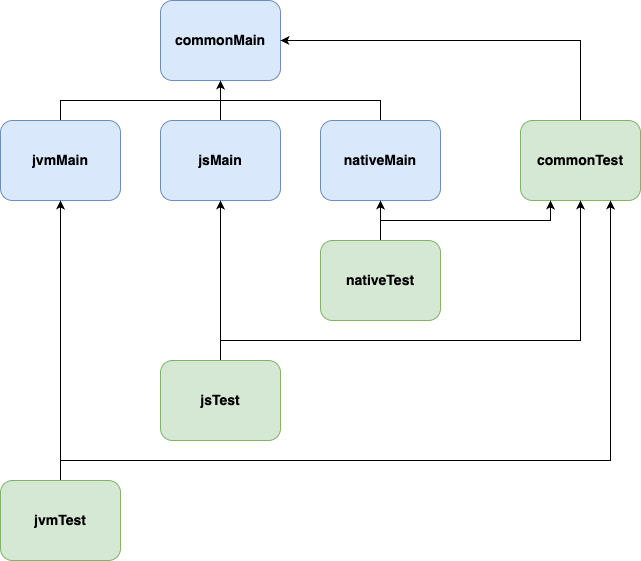
\includegraphics[width=0.95\textwidth]{charts/kmp-structure.drawio.png}
    \caption{Przykładowa struktura pojektu Kotlin Multiplatform [źródło:~opracowanie~własne]}
    \label{fig:kmp_project_structure}
\end{figure}

Następnie programista może utworzyć kolejne katalogi, które będą zawierać kod specyficzny dla docelowych platform.
Przykładowa struktura została przedstawiona na Rysunku \ref{fig:kmp_project_structure}, gdzie katalog commonMain jest wspóldzielony między JVM (jvmMain), JavaScript (jsMain) oraz platformy natywne (nativeMain).
Docelowe platformy (ang. targets) są deklarowane w konfiguracji Gradle \cite{kotlinMultiplatformDev}, a kod współdzielony jest przygotowywany wyłącznie dla nich.
Katalogi dla docelowych platform są wymagane, gdyż Kotlin nie zezwala na użycie specyficznych elementów danej platformy w katalogu współdzielonym.
Przykładem takiego elementu może być klasa ,,java.io.File'', która jest dostępna wyłącznie dla maszyny wirtualnej Javy.
Jej użycie w katalogu commonMain spowoduje błąd kompilacji.

Kotlin Multiplatform zawiera także integracje z testami oprogramowania.
Jest to szczególnie ważne dla tworzenia oprogramowania z wykorzystaniem AWS Lambda, gdzie testowanie może być skomplikowane (co było jednym z wniosków przeglądu literatury w Rozdziale \ref{chapter:przeglad_literatury}).
Testy dla kodu współdzielonego powinny być zapisane w katalogu ,,commonTest'', gdzie programista może użyć biblioteki kotlin.test \cite{kotlinMultiplatformDev}.
Następnie testy są uruchamiane dla każdej docelowej platformy.
Programista może także tworzyć przypadki testowe dla konkretnych platform, z użyciem technologii przez nie oferowanych.
Następuje tutaj analogiczne współdzielenie kodu jak dla katalogów ,,main'', co zostało także zawarte w Rysunku \ref{fig:kmp_project_structure}.

Specyficzne cechy Kotlina jak funkcjonalności języka, biblioteki czy projekt Kotlin Multiplatform mogą zapewnić znaczne wzrosty wydajności funkcji AWS Lambda.
Mimo, że Kotlin jest językiem wywodzącym się z Javy oferuje już możliwości, które mogą pozwolić na osiągnięcie niższych czasów odpowiedzi.
Dodatkowo, sposoby te nie zostały jeszcze przebadane. 
Dlatego Kotlin to obszar, który zasługuje na zawarcie go w badanich na temat wydajności AWS Lambda.

\section{Kotlin/JS}\label{chapter:kotlin_js}

\section{Kotlin/Native}\label{chapter:kotlin_native}

Bardzo skuteczną metodą optymalizacji wydajności może być rezygnacja z zarządzanych środowisk uruchomieniowych jak JVM.
Jedną z metod jest kompilacja do kodu natywnego, który uruchamiany jest bezpośrednio na systemie operacyjnym poza maszyną wirtualną.
Kotlin/Native oferuje zaawansową kompilację kodu Kotlin, który następnie może zostać uruchomiony w AWS Lambda z użyciem Amazon Linux.
W ramach rozdziału opisano sposób działania Kotlin/Native, jego możliwości i cechy, które mogą negatywnie wpłynąć na rozwój oprogramowania bezserwerowego.

Kluczowym elementami Kotlin/Native są kompilator oparty o LLVM oraz natywne implementacje bibliotek standardowych Kotlina \cite{kotlinlangKotlinDocs}.
Jak opisują Lattner i Adve \cite{1281665}, LLVM to framework kompilatora zaprojektowany do wspierania ciągłej i transparentnej analizy oraz transformacji programów.
Definiuje on wspólną, niskopoziomową reprezentację kodu w formie SSA (ang. Static Single Assignment) z systemem typów niezależnym od języka, co umożliwia implementację cech języków wysokiego poziomu. 
Głównym celem LLVM jest umożliwienie analizy i transformacji programu na różnych etapach jego życia, w tym w czasie kompilacji, linkowania, uruchomienia oraz w czasie bezczynności między uruchomieniami.
Jego użycie pozwala następnie na zbudowanie natywnych plików binarnych, które mogą zostać uruchomione bezpośrednio na docelowej platformie, dla której zostały skompilowane.
Wymaga to jednak dokładnego określenia systemu operacyjnego i architektury już w momencie kompilacji.

Kompilacja Kotlina do kodu natywnego otwiera przez KMP możliwość tworzenia samodzielnych programów wykonywalnych, które nie wymagają zewnętrznego środowiska uruchomieniowego.
Znajduje to zastosowanie w scenariuszach takich jak rozwój aplikacji mobilnych na platformę iOS, współdzielenie logiki biznesowej między różnymi platformami (np. Android i iOS) czy budowa narzędzi konsolowych.
Dlatego ważnym aspektem Kotlin/Native jest współdziałanie z istniejącym kodem natywnym.
Pozwala to na bezpośrednie wywoływanie funkcji z bibliotek napisanych w języku C, a na platformach firmy Apple również Objective-C \cite{kotlinlangKotlinDocs}.
Znacząco rozszerza to zakres dostępnych narzędzi i bibliotek, które mogą zostać użyte przez programistów.

Kotlin/Native oferuje wiele różnych platform docelowych, rozszerzając tym samym zakres zastosowań języka Kotlin.
Wśród wspieranych systemów docelowych znajdują się platformy Apple (takie jak macOS, iOS, watchOS, tvOS), Android, a także systemy z rodziny Windows oraz Linux \cite{kotlinlangKotlinDocs}.
Szczególnie istotnie dla usługi AWS Lambda są jednak platformy linuxowe.
Są to linuxX64 oraz linuxArm64, które pozwalają na uruchomienie kodu z użyciem odpowiednio architektur x86 oraz ARM.
Pozwala to następnie na ich bezpośrednie użycie w AWS Lambda, działającej bezpośrednio w systemie Amazon Linux.
Dzięki temu możliwa jest poprawa wydajności, szczególnie w aspekcie zimnych startów, które są znacznym wyzwaniem dla funkcji opartych o JVM.

Istotnym elementen funkcji bezserwerowych jest zarządzanie pamięcią, która wpływa bezpośrednio na koszty.
W przypadku Kotlin/Native, ewolucja modelu zarządzania pamięcią znacząco wpłynęła na jego użyteczność i możliwości optymalizacyjne.
Początkowa technologia ta opierała się na restrykcyjnym modelu z izolacją obiektów między wątkami \cite{kotlinlangKotlinDocs}.
Powodowało to skomplikowane zarządzanie stanem w operacjach współbieżnych.
Aktualnie, Kotlin/Native implementuje nowy menedżer pamięci.
Wprowadza on automatyczne zarządzanie pamięcią poprzez współbieżny, nieblokujący moduł zbierania śmieci (ang. garbage collector) \cite{kotlinlangKotlinDocs}.
Znacząco upraszcza to programowanie współbieżne, które teraz nie wymaga ręcznego zarządzania obiektami.
Mechanizm ten wprowadza intuicyjne współdzielenie stanu, które jest analogiczne do środowiska JVM, jednak bez konieczności kosztownej obsługi maszyny wirtualnej Java.

Mimo potencjalnych zysków w ramach wydajności, użycie Kotlin/Native może nieść utrudnienia w kontekście integracji z bibliotekami zewnętrznymi.
Język C nie jest oficjalnie wspierany jako język programowania AWS Lambda \cite{awsLambdaDeveloperGuide}, co wynika zapewne z jego niewielkiej popularności na tej platformie.
Współdziałanie z kodem natywnym w Kotlin/Native skupia się jednak na platformach klienckich, co nie musi być do końca użyteczne w zakresie AWS Lambda.
Amazon Web Services oferuje swoje SDK w języku C++, który nie jest jednak łatwo integrowalny z Kotlin/Native (w odróżnieniu od C i Objective-C).
Jest to ważny czynnik, który powinien być uwzględniony przez programistów projektujących aplikacje bezserwerowe.

% Plan
% 0. Wstęp

% 1. Jak to działa:
% - Opisać LLVM
% - Gdzie się głównie używa
% - Wspomnieć o interoperacyjności z C, Objective-C itp
% - Jakie platformy? (https://kotlinlang.org/docs/native-target-support.html#for-library-authors)

% 2. Zarządzanie pamięcią (https://kotlinlang.org/docs/native-memory-manager.html)

% 3. Wady - problem z dostępnością bibliotek
% - AWS SDK może poprzez C++ jednak może to wymagać większego nakładu pracy


\chapter{Wybrane metody optymalizacji}\label{chapter:wybrane_metody_optimalizacji}

% TODO: jakiś wstęp, typu jakich metod brakowało w przeglądzie. Podkreślić brak innych języków
\section{SnapStart}\label{chapter:snapstart}

Jednym z istotnych czynników wpływających na wydajność funkcji AWS Lambda implementowanych w ekosystemie Java jest zjawisko tzw. zimnego startu.
Wynika on z cyklu życia funkcji i etapu inicjalizacji (co zostało opisane w Rozdziale \ref{chapter:aws_lambda}).
W etap ten wchodzą procesy takie jak inicjalizacja maszyny wirtualnej Java czy uruchomienie statycznego kodu inicjującego \cite{awsLambdaDocs}.
W przypadku Javy zajmuje to więcej czasu niż dla innych języków (jak Python), co wydłuża zimne starty \cite{8605773}.
Znacząco oddziałuje to na wydajność funkcji, a może być szczególnie dotkliwe dla serwisów o niewielkiej aktywności.
W odpowiedzi na potrzebę minimalizacji tych negatywnych skutków Amazon Web Services wprowadziło mechanizm znany jako AWS Lambda SnapStart.
W ramach podrozdziału podjęto analizę tego rozwiązania w kontekście jego działania, zalet oraz ograniczeń. 

Mechanizm SnapStart istotnie modyfikuje tradycyjny cykl życia funkcji AWS Lambda.
Zasadnicza różnica polega na przeniesieniu kosztownego etapu inicjalizacji z momentu pierwszego wywołania funkcji na etap jej publikacji \cite{amazonSnapstartDeveloperGUide}.
Oznacza to, że inicjalizacja funkcji nie jest wykonywana w momencie zapytania użytkownika (co wywołuje zimny start), lecz w momencie wgrania nowej wersji funkcji (oraz kodu) przez programistę.
Inicjalizacja ta zawiera najdłuższe operacje dla rozwiązań Java jak utworzenie maszyny wirtualnej, załadowanie klas, czy wykonanie kodu inicjalizującego.
Następnie, tworzona jest zaszyfrowana ,,migawka'' (ang. snapshot) stanu pamięci i dysku w pełni gotowego środowiska wykonawczego.
Gdy funkcja jest następnie wywoływana po raz pierwszy, nie zachodzi już standardowy zimny start.
Zamiast tego środowisko jest odtwarzane z utworzonej migawki, co zostało przedstawione na Rysunku \ref{fig:aws_lambda_snapstart_process}.
Według dostawcy AWS metoda ta w optymalnych scenariuszach zmniejsza opóźnienie z kilku sekund do mniej niż sekundy \cite{amazonSnapstartDeveloperGUide}. 

\begin{figure}[h]
    \centering
    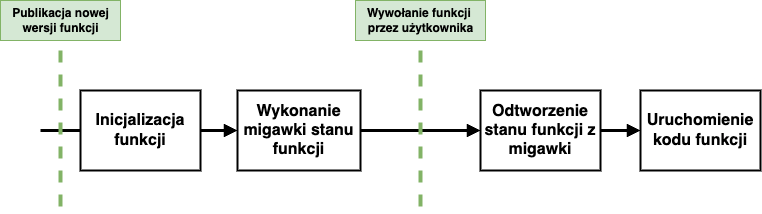
\includegraphics[width=0.95\textwidth]{charts/snapstart.png}
    \caption{Proces uruchomienia AWS Lambda z użyciem metody SnapStart [źródło:~opracowanie~własne]}
    \label{fig:aws_lambda_snapstart_process}
\end{figure}

Działanie tej metody jest technicznie możliwe dzięki użyciu środowiska wirtualizacji przez AWS Lambda.
Jak opisują Agache i inni autorzy \cite{246288} usługa Lambda do izolacji poszczególnych funkcji wykorzystuje dedykowane maszyny wirtualne typu microVM.
Są one zarządzane przez lekki monitor maszyn wirtualnych (ang. VMM) o nazwie Firecracker.
Posiada on cechy, które były kluczowe w minimalizacji problemu zimnego startu.
Po pierwsze, celowo rezygnuje on z emulacji zbędnych urządzeń (jak emulacja systemu BIOS czy rozbudowanych kontrolerów PCI) \cite{246288}.
Zmniejsza to złożoność i rozmiar stanu każdej maszyny wirtualnej. 
Dzięki temu wykonanie i odtworzenie migawki jest łatwiejsze.
Po drugie, Firecracker jest w pełni kontrolowany przez interfejs REST API \cite{246288}.
Umożliwia to precyzyjne zarządzanie całym cyklem życia każdej maszyny wirtualnej, włączając w to jej konfigurację, uruchomienie oraz zatrzymanie.
Pozwala to na określenie fazy inicjalizacji funkcji oraz wykonanie migawki w odpowiednim momencie.
Istotna jest również zapewniona przez Firecracker izolacja \cite{246288}, co gwarantuje bezpieczeństwo tworzenia i odtwarzania migawek.

Samo użycie metody SnapStart jest bardzo proste i nie wymaga od programisty dużego nakładu pracy.
Włączenie rozwiązania wymaga jedynie ustawienia odpowiedniej opcji podczas konfiguracji funkcji \cite{amazonSnapstartDeveloperGUide}.
Nie oznacza to jednak, że SnapStart jest odpowiedni dla wszystkich funkcji.
AWS podkreśla dwa typy aplikacji, które znacząco zyskają poprzez użycie SnapStart \cite{amazonSnapstartDeveloperGUide}.
Są nimi wrażliwe na opóźnienia interfejsy API i potoki przetwarzania danych.
Dodatkowo, metoda ta niesie za sobą pewne ograniczenia, które muszą zostać uwzględnione przed jej wdrożeniem.

Pierwszym aspektem jest kwestia unikalności stanu w funkcjach wykorzystujących SnapStart.
Jak analizują Brooker i inni autorzy \cite{brooker2021restoringuniquenessmicrovmsnapshots}, klonowanie migawek wprowadza fundamentalne wyzwanie związane z przywróceniem unikalności maszyn wirtualnych, co jest niezbędne do poprawnego generowania unikalnych identyfikatorów czy sekretów kryptograficznych.
Migawka zainicjowanego środowiska wykonywana jest jednorazowo, a następnie używana podczas wielu wywołań funkcji.
Może to stanowić duże zagrożenie dla programisty AWS Lambda, gdy potrzebuje on generować unikalne wartości jak identyfikatory (np. UUID) czy jednorazowe tokeny.
Narusza to znacznie poprawność logiki aplikacji oraz jej bezpieczeństwo.
Jedną z metod naprawy tego problemu jest generowanie wartości losowych wyłącznie w metodzie wywołującej funkcje (zamiast w bloku statycznym kodu) \cite{amazonSnapstartDeveloperGUide}.
Dodatkowo, ewentualne problemy z unikalnością funkcji SnapStart mogą zostać wykryte poprzez oprogramowanie SpotBugs \cite{SpotBugsProject}.
Narzędzie wykonuje statyczną analizę kodu, walidując go poprzez reguły zapewnione przez AWS.
Pozwala to programiście wykryć, a następnie naprawić fragmenty kodu powodujące problem z unikalnością.

Kolejnym istotnym wyzwaniem podczas rozwoju aplikacji z technologią SnapStart jest zarządzanie połączeniami sieciowymi \cite{amazonSnapstartDeveloperGUide}.
Połączenia nawiązane z zewnętrznymi usługami są standardową praktyką podczas tworzenia aplikacji AWS Lambda \cite{eismann2021reviewserverlessusecases}\cite{Ivanov_Petrova_2024}.
Problematyczne stają się jednak te połączenia sieciowe, które nawiązano podczas inicjalizacji funkcji. 
Ponieważ inicjalizacja odbywa się przed faktycznym przetworzeniem żądania użytkownika, upływający czas może sprawić, że w momencie odtworzenia funkcji połączenia te nie będą już aktywne.
Praktyką zalecaną przez AWS jest ponowne nawiązywanie lub dokładna walidacja istniejących połączeń \cite{amazonSnapstartDeveloperGUide}.
Powinno to być wykonane bezpośrednio w metodzie wywołującej funkcje lub z wykorzystaniem metody ,,afterRestore''.
Metoda ta jest wywoływana bezpośrednio po odtworzeniu migawki stanu funkcji.

Strategicznym czynnikiem usług bezserwerowych są koszty, zatem powinny być one uwzględnione także przed użyciem SnapStart.
Zgodnie z dokumentacją Amazon Web Services \cite{amazonSnapstartDeveloperGUide}, użycie SnapStart dla środowisk uruchomieniowych Java nie wiążą się z dodatkowymi kosztami.
Koszt wykonania funkcji z włączonym SnapStart nadal bazuje na standardowych rozliczeniach.
Składa się na niego liczba przetworzonych żądań oraz łączny czas trwania wykonań.

Podsumowując, mechanizm SnapStart stanowi prostą w aktywacji metodę redukcji czasu zimnych startów.
Sam mechanizm opiera się na wcześniejszym wykonaniu fazy inicjacji funkcji, a następnie wykonania migawki stanu.
W momencie wywołania funkcji stan ten może zostać odtworzony.
Znaczącą korzyścią metody jest brak dodatkowych kosztów.
Wiąże się ona jednak z istotnymi utrudnieniami (jak zarządzanie połączeniami sieciowymi i problem z unikalnością stanu).
Powinny być one uwzględnione przez programistę przed użyciem narzędzia.
\section{GraalVM}\label{chapter:graalvm}

Ważnym obszarem badań nad optymalizacją Javy i jej użycia w AWS Lambda, są technologie pozwalające na zmianę sposobu kompilacji i uruchamiana aplikacji.
Jedną z technologii, które zyskusje na popularności w tym zakresie, jest GraalVM.
Jest to możliwe m.in. dzięki użyciu kompilatora JIT (ang. Just-In-Time) w połączeniu z kompilacją AOT (ang. Ahead-Of-Time) \cite{8756917}.
GraalVM oferuje zaawansowaną architekturę pozwalającą na kompilację i uruchomienie aplikacji w postaci obrazów natywnych.
Stanowi to alternatywę dla klasycznej maszyny wirtualnej Javy, a dodatkowo skupia się na jej wydajności.
Poniższy podrozdział poświęcono analizie działania omawianego rozwiązania, jego zalet i słabych stron.

Kluczowym mechanizmem GraalVM jest kompilacja AOT (ang. Ahead-Of-Time) do postaci tzw. obrazów natywnych (ang. native images) \cite{8756917}.
Ma to bezpośredni wpływ na wydajność działania aplikacji.
W modelu tradycyjnym, kod bajtowy Java jest interpretowany i kompilowany dynamicznie przez maszynę wirtualną w trakcie działania aplikacji.
Podejście AOT przenosi znaczną część z tych operacji na etap budowania artefaktu. 
Istotnym elementem tego procesu jest agresywna, statyczna analiza kodu \cite{9245290}, w celu identyfikacji osiągalnych w trakcie działania części.
Pozwala to na odrzucenie nieużywanych fragmentów kodu (np. z używanych bibliotek), co pozwala na zmniejszenie wielkości obrazu natywnego.
Aspekt ten może być kluczowy w kontekście AWS Lambda, ze względu na wpływ wielkości artefaktu na wydajność \cite{8116416}.
Po analizie kodu, dokonywana jest inicjalizacja klas, a stan aplikacji, w tym częściowo zainicjalizowana sterta, jest utrwalany.
W celu lepszej optymalizacji, operacje te są powtarzane, co zostało przedstawione na Rysunku \ref{fig:graalvm_build_process}.

Jako wynik kompilacji powstaje samodzielny, zoptymalizowany plik binarny.
Nie wymaga on do uruchomienia pełnej maszyny wirtualnej Java, a jedynie minimalnego środowiska wykonawczego dostarczanego przez SubstrateVM, będącego częścią GraalVM \cite{8756917}.
Różnica ta ma fundamentalne znaczenie w kontekście wydajności AWS Lambda.
Eliminowana jest konieczność wykonywania czasochłonnych operacji typowych dla startu tradycyjnej maszyny wirtualnej Java, takich jak ładowanie klas czy jej inicjalizacja.
Wszystkie te zadania zostały już wykonane wcześniej, w procesie budowy obrazu natywnego.
Dzięki temu tworzona przez programistę funkcja AWS Lambda nie będzie operować w zarządzanym środowisku Java.
Zamiast tego, usługi muszą opierać się o niestandardowe środowiska wykonawcze, oferujące wyłącznie system operacyjny (Amazon Linux 2023 lub Amazon Linux 2) \cite{awsLambdaDeveloperGuide}.
Ich użycie pozwala także na realizację drugiej zalety GraalVM, czyli redukcji zapotrzebowania na pamięć operacyjną \cite{9245290}.

Pomimo pozytywnego wpływu na wydajność, zastosowanie kompilacji AOT w GraalVM wiąże się także z ograniczeniami.
Jednym z nich jest obsługa dynamicznych cech Javy, takich jak refleksja (ang. reflection), dynamiczne proxy, serializacja czy natywny interfejs Java (JNI)
Wynika to z faktu użycia agresywnej statycznej analizy kodu.
Napotyka ona trudności w przewidzeniu wszystkich dynamicznie ładowanych klas, pól i metod, które nie są jawnie osiągalne w kodzie źródłowym.
Problem ten wymaga użycia dodatkowych mechanizmów GraalVM \cite{graalvm-reflection-jdk21}.
Polegają one na przygotowaniu dodatkowych metadanych dla klas, co wymaga jednak dodatkowej obsługi.

\begin{figure}
    \centering
    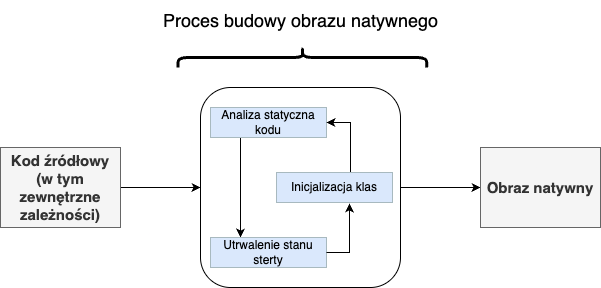
\includegraphics[width=0.95\textwidth]{charts/graalvm-build-process.drawio.png}
    \caption{Uproszczony proces budowy obrazu natywnego GraalVM [źródło:~opracowanie~własne]}
    \label{fig:graalvm_build_process}
\end{figure}

Kolejnym aspektem, który może negatywnie wpłynąć na rozwój oprogramowania przy użyciu GraalVM, jest czasochłonność procesu kompilacji.
Generowanie w pełni zoptymalizowanego obrazu natywnego jest operacją bardziej złożoną niż standardowa kompilacja kodu Javy do postaci bajtowej.
W praktyce oznacza to, że proces budowania artefaktu dla funkcji AWS Lambda może trwać odczuwalnie dłużej.
Może mieć to znaczący wpływ na rozwój oprogramowania, szczególnie w przypadku częstych iteracji i tworzenia nowych wersji funkcji.
Dłuższy czas kompilacji może także wpłynąć na ogólną efektywność procesów ciągłej integracji i ciągłego dostarczania (ang. CI/CD).

Jednym z sposobów poprawy doświadczeń programistów przy pracy z GraalVM, jest użycie odpowiednich frameworków.
Jednym z nich jest Quarkus \cite{9245290}, który został zaprojektowany z myślą o środowiskach chmurowych.
Kluczową cechą Quarkusa jest przeniesienie jak największej liczby operacji inicjalizacyjnych i konfiguracyjnych na etap budowania aplikacji.
Obejmuje to między innymi wstrzykiwanie zależności, przetwarzanie adnotacji oraz konfigurację rozszerzeń. 
Dzięki temu, w czasie budowania obrazu natywnego, Quarkus jest w stanie przeprowadzić szczegółową analizę aplikacji.
Poprzez użycie odpowiednich annotacji pozwala on na oznaczenie klas niezbędnych dla mechanizmów refleksji czy proxy \cite{quarkus-docs}.
Dzięki temu jest on w stanie automatycznie wygenerować niezbędne metadane dla klas.
Dane te następnie pozwalają na użycie wspomnianych mechanizmów w GraalVM.
Innymi, konkurencyjnymi do Quarkusa frameworkami, które oferują wsparcie dla obrazów natywnych są Helidon i Micronaut \cite{9245290}.
Ich popularność wskazuje na wysokie zainteresowanie takimi technologiami w społeczności programistów Java, dlatego jest to interesujący kierunek rozwoju dla funkcji AWS Lambda.

\section{Kotlin}\label{chapter:kotlin_multiplatform}

W ramach systematycznego przeglądu literatury (przedstawionego w Rozdziale \ref{chapter:przeglad_literatury}) zauważono, że aktualne badania skupiają się wyłącznie na języku Java.
Pomijają one jednak inne języki z ekosystemu Java, także oparte o maszynę wirtualną Java (ang. JVM).
Tymczasem na popularności zyskują alternatywne języki ekosystemu Javy.
Wśród nich na szczególną uwagę zasługuje Kotlin, rozwijany przez firmę JetBrains.
Jest on oficjalnie wspierany przez Google jako język programowania dla platformy Android, co wskazuje na jego solidne zastosowanie w tych systemach.
Coraz większe uznanie zyskuje także jako działający po stronie serwera. 
Dlatego język ten jest interesującym obszarem badań w kontekście AWS Lambda.
W tym rozdziale przedstawiony zostanie język programowania Kotlin, w tym jego zastosowanie w kontekście funkcji AWS Lambda.

Jednym z kluczowych czynników, które zwiększają popularność Kotlina, jest jego łatwa nauka przez programistów Javy.
Dodatkowo, istnieje możliwość łatwej intergracji kodu napisanego w Kotlinie z istniejącym oprogramowaniem Java \cite{kotlinlangKotlinDocs}.
Te cechy czynią go interesującym kandydatem do analizy w kontekście optymalizacji wydajności rozwiązań dla usługi AWS Lambda. 
Dla zespołów programistycznych może stanowić on wartościowe rozszerzenie dotychczasowych możliwości. 
Kotlin oferuje bowiem alternatywę lub uzupełnienie dla tradycyjnie stosowanej Javy.

Kwestia wydajności Kotlina w porównaniu do Javy jest przedmiotem dyskusji. 
Jednak badania dotyczą najczęściej ich zastosowań w kontekście aplikacji mobilnych.
Gajek i inni autorzy \cite{Gajek_Plechawska-Wójcik_2024} przeanalizowali wydajność obu języków, poprzez użycie gry mobilnej uruchomionej na systemie Android.
Wykazali oni, że w testowanym scenariuszu Java osiągnęła nieznacznie lepszą wydajność pod względem zużycia zasobów CPU i RAM.
Było to jednak zastosowanie mobilne, a same różnice nie były znaczne.
Należy jednak podkreślić, że warunki mobilne mogą być inne niż w systemach działających w usłudze AWS Lambda.
Sam język Kotlin posiada mechanizmy, które mogą pozytywnie wpłynąć na wydajność.

Funkcje inline (ang. inline functions) w Kotlinie mogą przyczynić się do redukcji narzutu wydajności podczas wywołań funkcji.
Mechanizm ten polega na wstawieniu kodu ciała funkcji bezpośrednio w miejsce jej wywołania \cite{kotlinlangKotlinDocs}.
Jest to wykonywane w momencie kompilacji, a programista może określić, które funkcje powinny być w ten sposób optymalizowane.
Eliminuje to koszt ich wywołania, co jest szczególnie przydatne w przypadku małych, często używanych funkcji.
Dodatkowo, język pozwala na przekazywanie funkcji jako parametrów, na przykład w kolekcjach i metodach jak filtrowanie.
W tych sytuacjach użycie funkcji inline może znacząco zmniejszyć liczbę operacji.
Pozytywny wpływ mechanizmu inline został przedstawiony przez Bergstrom i innych autorów \cite{DBLP:journals/corr/BergstromFRS13}, gdzie jego użycie zmniejszyło czas wykonywania programów nawet do 8\%.

Innym istotnym elementem Kotlina wspierającym wydajność są korutyny (ang. coroutines).
Mogą być one użyteczne zwłaszcza w kontekście operacji wejścia-wyjścia (I/O).
Systemy oparte o usługę AWS Lambda często integrowane są z zewnętrznymi serwisami (co zostało zauważone w ramach przeglądu literatury w Rozdziale \ref{chapter:przeglad_literatury}).
Wymaga to komunikacji opartej o operacje sieciowe.
Tradycyjne podejście oparte na wątkach może konsumować dużą ilość zasobów serwera i prowadzić do blokowania wykonania.
Korutyny pozwalają na pisanie asynchronicznego, nieblokującego kodu w sposób bardziej sekwencyjny i czytelny \cite{kotlinlangKotlinDocs}.
Na lepszą wydajność korutyn w porównaniu z tradycyjnymi wątkami wskazali Beronić i inni autorzy \cite{9803765}.

Implementacja mechanizmów poprawiających wydajność w języku programowania, pozwala następnie na ich użycie w bibliotekach, które są wykorzystywane przez programistów.
Język Kotlin oferuje ciekawy ekosystem bibliotek, przeznaczonych na przykład do tworzenia aplikacji działających po stronie serwera.
Są to biblioteki jak http4k czy ktor.
Ktor to framework zaprojektowany do budowy asynchronicznych aplikacji serwerowych i klienckich, rozwijany przez firmę JetBrains.
Jest on oparty w pełni o język Kotlin, a jego kluczową cechą jest natywne wsparcie dla korutyn.
Z kolei http4k kładzie nacisk na prostotę i minimalizm.
Architektura http4k opiera się na koncepcji funkcji jako podstawowych bloków aplikacji \cite{http4kCoreDocs}, co naturalnie współgra z modelem serverless i AWS Lambda.
Samo narzędzie rezyguje z mechanizmów refleksji \cite{http4kCoreDocs}, co może mieć pozytywny wpływ na wydajność.

Rosnące znaczenie Kotlin dostrzega także Amazon Web Service, które oferuje bibliotekę AWS SDK dla Kotlina \cite{awsSDKForKotlinDeveloperGuide}.
Jej celem jest zapewnienie programistom możliwości interakcji z usługami AWS w sposób naturalny dla tego języka.
SDK ten został zaprojektowany od podstaw z myślą o Kotlinie, co przejawia się między innymi w wykorzystaniu korutyn do obsługi operacji asynchronicznych.

Duży wpływ na wydajność funkcji AWS Lambda ma wybrany język programowania \cite{8605773}\cite{Cordingly2020704}.
Wynika to na przykład z różnych przypadków biznesowych i operacji, które muszą wykonywać.
Mimo to, często muszą one dzielić wspólny kod \cite{8116416}, co wskazuje na potrzebę wykorzystania mechanizmów, które to umożliwą.
Z tego powodu bardzo interesującą dla AWS Lambda i jej wydajności, może okazać się inicjatywa Kotlin Multiplatform.
KMP (Kotlin Multiplatform) to projekt, który powstał w szczególności dla aplikacji mobilnych.
Pozwala on na kompilację lub translację tego samego kodu Kotlin do użycia na różnych platformach.
Mogą to być na przykład Android, iOS, aplikacje desktopowe (JVM) lub webowe (JavaScript, Web Assembly) \cite{kotlinlangKotlinDocs}.
Oferuje to możliwość dzielenia kodu (np. logiki biznesowej) pomiędzy różnymi platformami, jednak przy możliwości zachowania natywnych komponentów widoku.

Mimo głównego przypadku użycia jakim są aplikacje klienckie, Kotlin Multiplatform może być obiecującym rozwiązaniem dla AWS Lambda.
Po pierwsze oferuje on możliwość translacji kodu Kotlin do JavaScript oraz kompilację do natywnych plików binarnych (opcje te zostaną przedstawione jako osobne metody w kolejnych rozdziałach).
Pozwala to na ominięcie różnych niedogodności wynikających z użycia maszyny wirtualnej Javy.
Jednak zachowane są przy tym zalety języka oraz wspiera to użycie już istniejących umiejętności programistów języków rodziny JVM.
Po drugie, kod w KMP może być dzielony pomiędzy platformami.
Umożliwia to bardzo elastyczny wybór środowiska uruchomieniowego AWS Lambda w ramach pojedynczego systemu.
Jednocześnie, część kodu może być współdzielona między wszystkie funkcje niezależnie od wybranej platformy.
Może to na przykład oznaczać, że klasy implementujące pewne struktury oraz zasady wynikające z reguł biznesowych, będą mogły być używane przez funkcje działające zarówno poprzez JavaScript, JVM, jak i natywne pliki binarne. 

Jednym z czynników, które mogą być modyfikowane już podczas działania usług AWS Lambda jest pamięć.
Jej rozmiar może być dostosowywany w zależności od wydajności monitorowanej funkcji.
Użycie Kotlin Multiplatform pozwala na rozszerzenie tej metody.
W zależności od obserwowanych parametrów (jak czas odpowiedzi lub opóźnienia zimnych startów) możliwe jest ponowne wykorzystanie tego samego kodu i budowa funkcji działającej na innej platformie.
Przykładowo, po wdrożeniu funkcji działającej z użyciem JVM, może pojawić się potrzeba redukcji czasu zimnych startów.
W takim wypadku Kotlin Multiplatform umożliwia translację kodu do JavaScript, który pozwoli na redukcję czasu inicjalizacji AWS Lambda.

Współdzielenie kodu pomiędzy platformami jest możliwe dzięki strukturze, którą oferuje Kotlin Multiplatform.
Została ona opisana przez firmę JetBrains w ramach dokumentacji KMP \cite{kotlinMultiplatformDev}.
Jej głównym elementem jest katalog ,,commonMain'', który jest współdzielony pomiędzy wszystkimi platformami.
Kompilator używa kodu współdzielonego jako dane wejściowe, aby w rezultacie utworzyć zestaw plików binarnych specyficznych dla danej platformy.
Mogą to być na przykład pliki .class dla maszyny wirtualnej Javy, czy natywne pliki wykonywalne (np. dla platformy Linux).

\begin{figure}[h]
    \centering
    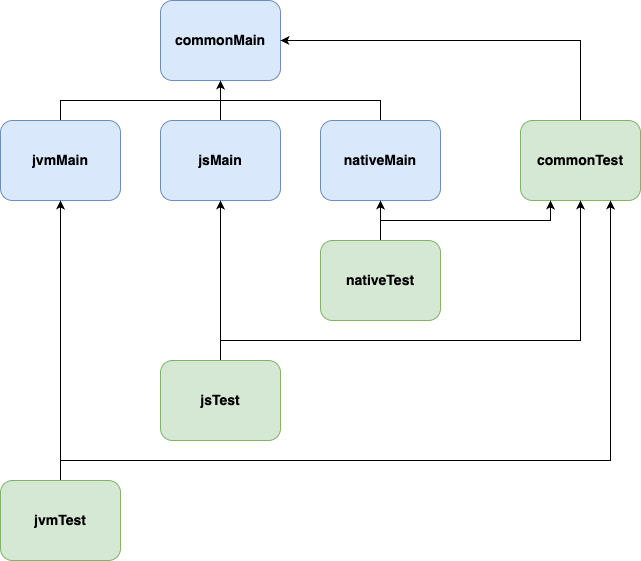
\includegraphics[width=0.95\textwidth]{charts/kmp-structure.drawio.png}
    \caption{Przykładowa struktura pojektu Kotlin Multiplatform [źródło:~opracowanie~własne]}
    \label{fig:kmp_project_structure}
\end{figure}

Następnie programista może utworzyć kolejne katalogi, które będą zawierać kod specyficzny dla docelowych platform.
Przykładowa struktura została przedstawiona na Rysunku \ref{fig:kmp_project_structure}, gdzie katalog commonMain jest wspóldzielony między JVM (jvmMain), JavaScript (jsMain) oraz platformy natywne (nativeMain).
Docelowe platformy (ang. targets) są deklarowane w konfiguracji Gradle \cite{kotlinMultiplatformDev}, a kod współdzielony jest przygotowywany wyłącznie dla nich.
Katalogi dla docelowych platform są wymagane, gdyż Kotlin nie zezwala na użycie specyficznych elementów danej platformy w katalogu współdzielonym.
Przykładem takiego elementu może być klasa ,,java.io.File'', która jest dostępna wyłącznie dla maszyny wirtualnej Javy.
Jej użycie w katalogu commonMain spowoduje błąd kompilacji.

Kotlin Multiplatform zawiera także integracje z testami oprogramowania.
Jest to szczególnie ważne dla tworzenia oprogramowania z wykorzystaniem AWS Lambda, gdzie testowanie może być skomplikowane (co było jednym z wniosków przeglądu literatury w Rozdziale \ref{chapter:przeglad_literatury}).
Testy dla kodu współdzielonego powinny być zapisane w katalogu ,,commonTest'', gdzie programista może użyć biblioteki kotlin.test \cite{kotlinMultiplatformDev}.
Następnie testy są uruchamiane dla każdej docelowej platformy.
Programista może także tworzyć przypadki testowe dla konkretnych platform, z użyciem technologii przez nie oferowanych.
Następuje tutaj analogiczne współdzielenie kodu jak dla katalogów ,,main'', co zostało także zawarte w Rysunku \ref{fig:kmp_project_structure}.

Specyficzne cechy Kotlina jak funkcjonalności języka, biblioteki czy projekt Kotlin Multiplatform mogą zapewnić znaczne wzrosty wydajności funkcji AWS Lambda.
Mimo, że Kotlin jest językiem wywodzącym się z Javy oferuje już możliwości, które mogą pozwolić na osiągnięcie niższych czasów odpowiedzi.
Dodatkowo, sposoby te nie zostały jeszcze przebadane. 
Dlatego Kotlin to obszar, który zasługuje na zawarcie go w badanich na temat wydajności AWS Lambda.

\section{Kotlin/JS}\label{chapter:kotlin_js}

\section{Kotlin/Native}\label{chapter:kotlin_native}

Bardzo skuteczną metodą optymalizacji wydajności może być rezygnacja z zarządzanych środowisk uruchomieniowych jak JVM.
Jedną z metod jest kompilacja do kodu natywnego, który uruchamiany jest bezpośrednio na systemie operacyjnym poza maszyną wirtualną.
Kotlin/Native oferuje zaawansową kompilację kodu Kotlin, który następnie może zostać uruchomiony w AWS Lambda z użyciem Amazon Linux.
W ramach rozdziału opisano sposób działania Kotlin/Native, jego możliwości i cechy, które mogą negatywnie wpłynąć na rozwój oprogramowania bezserwerowego.

Kluczowym elementami Kotlin/Native są kompilator oparty o LLVM oraz natywne implementacje bibliotek standardowych Kotlina \cite{kotlinlangKotlinDocs}.
Jak opisują Lattner i Adve \cite{1281665}, LLVM to framework kompilatora zaprojektowany do wspierania ciągłej i transparentnej analizy oraz transformacji programów.
Definiuje on wspólną, niskopoziomową reprezentację kodu w formie SSA (ang. Static Single Assignment) z systemem typów niezależnym od języka, co umożliwia implementację cech języków wysokiego poziomu. 
Głównym celem LLVM jest umożliwienie analizy i transformacji programu na różnych etapach jego życia, w tym w czasie kompilacji, linkowania, uruchomienia oraz w czasie bezczynności między uruchomieniami.
Jego użycie pozwala następnie na zbudowanie natywnych plików binarnych, które mogą zostać uruchomione bezpośrednio na docelowej platformie, dla której zostały skompilowane.
Wymaga to jednak dokładnego określenia systemu operacyjnego i architektury już w momencie kompilacji.

Kompilacja Kotlina do kodu natywnego otwiera przez KMP możliwość tworzenia samodzielnych programów wykonywalnych, które nie wymagają zewnętrznego środowiska uruchomieniowego.
Znajduje to zastosowanie w scenariuszach takich jak rozwój aplikacji mobilnych na platformę iOS, współdzielenie logiki biznesowej między różnymi platformami (np. Android i iOS) czy budowa narzędzi konsolowych.
Dlatego ważnym aspektem Kotlin/Native jest współdziałanie z istniejącym kodem natywnym.
Pozwala to na bezpośrednie wywoływanie funkcji z bibliotek napisanych w języku C, a na platformach firmy Apple również Objective-C \cite{kotlinlangKotlinDocs}.
Znacząco rozszerza to zakres dostępnych narzędzi i bibliotek, które mogą zostać użyte przez programistów.

Kotlin/Native oferuje wiele różnych platform docelowych, rozszerzając tym samym zakres zastosowań języka Kotlin.
Wśród wspieranych systemów docelowych znajdują się platformy Apple (takie jak macOS, iOS, watchOS, tvOS), Android, a także systemy z rodziny Windows oraz Linux \cite{kotlinlangKotlinDocs}.
Szczególnie istotnie dla usługi AWS Lambda są jednak platformy linuxowe.
Są to linuxX64 oraz linuxArm64, które pozwalają na uruchomienie kodu z użyciem odpowiednio architektur x86 oraz ARM.
Pozwala to następnie na ich bezpośrednie użycie w AWS Lambda, działającej bezpośrednio w systemie Amazon Linux.
Dzięki temu możliwa jest poprawa wydajności, szczególnie w aspekcie zimnych startów, które są znacznym wyzwaniem dla funkcji opartych o JVM.

Istotnym elementen funkcji bezserwerowych jest zarządzanie pamięcią, która wpływa bezpośrednio na koszty.
W przypadku Kotlin/Native, ewolucja modelu zarządzania pamięcią znacząco wpłynęła na jego użyteczność i możliwości optymalizacyjne.
Początkowa technologia ta opierała się na restrykcyjnym modelu z izolacją obiektów między wątkami \cite{kotlinlangKotlinDocs}.
Powodowało to skomplikowane zarządzanie stanem w operacjach współbieżnych.
Aktualnie, Kotlin/Native implementuje nowy menedżer pamięci.
Wprowadza on automatyczne zarządzanie pamięcią poprzez współbieżny, nieblokujący moduł zbierania śmieci (ang. garbage collector) \cite{kotlinlangKotlinDocs}.
Znacząco upraszcza to programowanie współbieżne, które teraz nie wymaga ręcznego zarządzania obiektami.
Mechanizm ten wprowadza intuicyjne współdzielenie stanu, które jest analogiczne do środowiska JVM, jednak bez konieczności kosztownej obsługi maszyny wirtualnej Java.

Mimo potencjalnych zysków w ramach wydajności, użycie Kotlin/Native może nieść utrudnienia w kontekście integracji z bibliotekami zewnętrznymi.
Język C nie jest oficjalnie wspierany jako język programowania AWS Lambda \cite{awsLambdaDeveloperGuide}, co wynika zapewne z jego niewielkiej popularności na tej platformie.
Współdziałanie z kodem natywnym w Kotlin/Native skupia się jednak na platformach klienckich, co nie musi być do końca użyteczne w zakresie AWS Lambda.
Amazon Web Services oferuje swoje SDK w języku C++, który nie jest jednak łatwo integrowalny z Kotlin/Native (w odróżnieniu od C i Objective-C).
Jest to ważny czynnik, który powinien być uwzględniony przez programistów projektujących aplikacje bezserwerowe.

% Plan
% 0. Wstęp

% 1. Jak to działa:
% - Opisać LLVM
% - Gdzie się głównie używa
% - Wspomnieć o interoperacyjności z C, Objective-C itp
% - Jakie platformy? (https://kotlinlang.org/docs/native-target-support.html#for-library-authors)

% 2. Zarządzanie pamięcią (https://kotlinlang.org/docs/native-memory-manager.html)

% 3. Wady - problem z dostępnością bibliotek
% - AWS SDK może poprzez C++ jednak może to wymagać większego nakładu pracy


\chapter{Wybrane metody optymalizacji}\label{chapter:wybrane_metody_optimalizacji}

% TODO: jakiś wstęp, typu jakich metod brakowało w przeglądzie. Podkreślić brak innych języków
\section{SnapStart}\label{chapter:snapstart}

Jednym z istotnych czynników wpływających na wydajność funkcji AWS Lambda implementowanych w ekosystemie Java jest zjawisko tzw. zimnego startu.
Wynika on z cyklu życia funkcji i etapu inicjalizacji (co zostało opisane w Rozdziale \ref{chapter:aws_lambda}).
W etap ten wchodzą procesy takie jak inicjalizacja maszyny wirtualnej Java czy uruchomienie statycznego kodu inicjującego \cite{awsLambdaDocs}.
W przypadku Javy zajmuje to więcej czasu niż dla innych języków (jak Python), co wydłuża zimne starty \cite{8605773}.
Znacząco oddziałuje to na wydajność funkcji, a może być szczególnie dotkliwe dla serwisów o niewielkiej aktywności.
W odpowiedzi na potrzebę minimalizacji tych negatywnych skutków Amazon Web Services wprowadziło mechanizm znany jako AWS Lambda SnapStart.
W ramach podrozdziału podjęto analizę tego rozwiązania w kontekście jego działania, zalet oraz ograniczeń. 

Mechanizm SnapStart istotnie modyfikuje tradycyjny cykl życia funkcji AWS Lambda.
Zasadnicza różnica polega na przeniesieniu kosztownego etapu inicjalizacji z momentu pierwszego wywołania funkcji na etap jej publikacji \cite{amazonSnapstartDeveloperGUide}.
Oznacza to, że inicjalizacja funkcji nie jest wykonywana w momencie zapytania użytkownika (co wywołuje zimny start), lecz w momencie wgrania nowej wersji funkcji (oraz kodu) przez programistę.
Inicjalizacja ta zawiera najdłuższe operacje dla rozwiązań Java jak utworzenie maszyny wirtualnej, załadowanie klas, czy wykonanie kodu inicjalizującego.
Następnie, tworzona jest zaszyfrowana ,,migawka'' (ang. snapshot) stanu pamięci i dysku w pełni gotowego środowiska wykonawczego.
Gdy funkcja jest następnie wywoływana po raz pierwszy, nie zachodzi już standardowy zimny start.
Zamiast tego środowisko jest odtwarzane z utworzonej migawki, co zostało przedstawione na Rysunku \ref{fig:aws_lambda_snapstart_process}.
Według dostawcy AWS metoda ta w optymalnych scenariuszach zmniejsza opóźnienie z kilku sekund do mniej niż sekundy \cite{amazonSnapstartDeveloperGUide}. 

\begin{figure}[h]
    \centering
    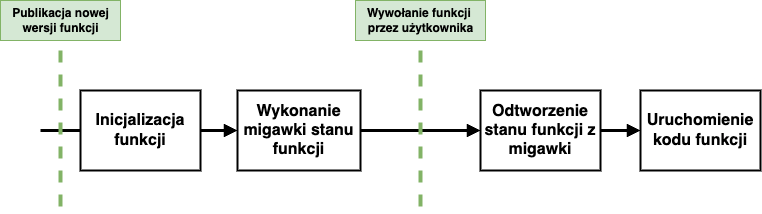
\includegraphics[width=0.95\textwidth]{charts/snapstart.png}
    \caption{Proces uruchomienia AWS Lambda z użyciem metody SnapStart [źródło:~opracowanie~własne]}
    \label{fig:aws_lambda_snapstart_process}
\end{figure}

Działanie tej metody jest technicznie możliwe dzięki użyciu środowiska wirtualizacji przez AWS Lambda.
Jak opisują Agache i inni autorzy \cite{246288} usługa Lambda do izolacji poszczególnych funkcji wykorzystuje dedykowane maszyny wirtualne typu microVM.
Są one zarządzane przez lekki monitor maszyn wirtualnych (ang. VMM) o nazwie Firecracker.
Posiada on cechy, które były kluczowe w minimalizacji problemu zimnego startu.
Po pierwsze, celowo rezygnuje on z emulacji zbędnych urządzeń (jak emulacja systemu BIOS czy rozbudowanych kontrolerów PCI) \cite{246288}.
Zmniejsza to złożoność i rozmiar stanu każdej maszyny wirtualnej. 
Dzięki temu wykonanie i odtworzenie migawki jest łatwiejsze.
Po drugie, Firecracker jest w pełni kontrolowany przez interfejs REST API \cite{246288}.
Umożliwia to precyzyjne zarządzanie całym cyklem życia każdej maszyny wirtualnej, włączając w to jej konfigurację, uruchomienie oraz zatrzymanie.
Pozwala to na określenie fazy inicjalizacji funkcji oraz wykonanie migawki w odpowiednim momencie.
Istotna jest również zapewniona przez Firecracker izolacja \cite{246288}, co gwarantuje bezpieczeństwo tworzenia i odtwarzania migawek.

Samo użycie metody SnapStart jest bardzo proste i nie wymaga od programisty dużego nakładu pracy.
Włączenie rozwiązania wymaga jedynie ustawienia odpowiedniej opcji podczas konfiguracji funkcji \cite{amazonSnapstartDeveloperGUide}.
Nie oznacza to jednak, że SnapStart jest odpowiedni dla wszystkich funkcji.
AWS podkreśla dwa typy aplikacji, które znacząco zyskają poprzez użycie SnapStart \cite{amazonSnapstartDeveloperGUide}.
Są nimi wrażliwe na opóźnienia interfejsy API i potoki przetwarzania danych.
Dodatkowo, metoda ta niesie za sobą pewne ograniczenia, które muszą zostać uwzględnione przed jej wdrożeniem.

Pierwszym aspektem jest kwestia unikalności stanu w funkcjach wykorzystujących SnapStart.
Jak analizują Brooker i inni autorzy \cite{brooker2021restoringuniquenessmicrovmsnapshots}, klonowanie migawek wprowadza fundamentalne wyzwanie związane z przywróceniem unikalności maszyn wirtualnych, co jest niezbędne do poprawnego generowania unikalnych identyfikatorów czy sekretów kryptograficznych.
Migawka zainicjowanego środowiska wykonywana jest jednorazowo, a następnie używana podczas wielu wywołań funkcji.
Może to stanowić duże zagrożenie dla programisty AWS Lambda, gdy potrzebuje on generować unikalne wartości jak identyfikatory (np. UUID) czy jednorazowe tokeny.
Narusza to znacznie poprawność logiki aplikacji oraz jej bezpieczeństwo.
Jedną z metod naprawy tego problemu jest generowanie wartości losowych wyłącznie w metodzie wywołującej funkcje (zamiast w bloku statycznym kodu) \cite{amazonSnapstartDeveloperGUide}.
Dodatkowo, ewentualne problemy z unikalnością funkcji SnapStart mogą zostać wykryte poprzez oprogramowanie SpotBugs \cite{SpotBugsProject}.
Narzędzie wykonuje statyczną analizę kodu, walidując go poprzez reguły zapewnione przez AWS.
Pozwala to programiście wykryć, a następnie naprawić fragmenty kodu powodujące problem z unikalnością.

Kolejnym istotnym wyzwaniem podczas rozwoju aplikacji z technologią SnapStart jest zarządzanie połączeniami sieciowymi \cite{amazonSnapstartDeveloperGUide}.
Połączenia nawiązane z zewnętrznymi usługami są standardową praktyką podczas tworzenia aplikacji AWS Lambda \cite{eismann2021reviewserverlessusecases}\cite{Ivanov_Petrova_2024}.
Problematyczne stają się jednak te połączenia sieciowe, które nawiązano podczas inicjalizacji funkcji. 
Ponieważ inicjalizacja odbywa się przed faktycznym przetworzeniem żądania użytkownika, upływający czas może sprawić, że w momencie odtworzenia funkcji połączenia te nie będą już aktywne.
Praktyką zalecaną przez AWS jest ponowne nawiązywanie lub dokładna walidacja istniejących połączeń \cite{amazonSnapstartDeveloperGUide}.
Powinno to być wykonane bezpośrednio w metodzie wywołującej funkcje lub z wykorzystaniem metody ,,afterRestore''.
Metoda ta jest wywoływana bezpośrednio po odtworzeniu migawki stanu funkcji.

Strategicznym czynnikiem usług bezserwerowych są koszty, zatem powinny być one uwzględnione także przed użyciem SnapStart.
Zgodnie z dokumentacją Amazon Web Services \cite{amazonSnapstartDeveloperGUide}, użycie SnapStart dla środowisk uruchomieniowych Java nie wiążą się z dodatkowymi kosztami.
Koszt wykonania funkcji z włączonym SnapStart nadal bazuje na standardowych rozliczeniach.
Składa się na niego liczba przetworzonych żądań oraz łączny czas trwania wykonań.

Podsumowując, mechanizm SnapStart stanowi prostą w aktywacji metodę redukcji czasu zimnych startów.
Sam mechanizm opiera się na wcześniejszym wykonaniu fazy inicjacji funkcji, a następnie wykonania migawki stanu.
W momencie wywołania funkcji stan ten może zostać odtworzony.
Znaczącą korzyścią metody jest brak dodatkowych kosztów.
Wiąże się ona jednak z istotnymi utrudnieniami (jak zarządzanie połączeniami sieciowymi i problem z unikalnością stanu).
Powinny być one uwzględnione przez programistę przed użyciem narzędzia.
\section{GraalVM}\label{chapter:graalvm}

Ważnym obszarem badań nad optymalizacją Javy i jej użycia w AWS Lambda, są technologie pozwalające na zmianę sposobu kompilacji i uruchamiana aplikacji.
Jedną z technologii, które zyskusje na popularności w tym zakresie, jest GraalVM.
Jest to możliwe m.in. dzięki użyciu kompilatora JIT (ang. Just-In-Time) w połączeniu z kompilacją AOT (ang. Ahead-Of-Time) \cite{8756917}.
GraalVM oferuje zaawansowaną architekturę pozwalającą na kompilację i uruchomienie aplikacji w postaci obrazów natywnych.
Stanowi to alternatywę dla klasycznej maszyny wirtualnej Javy, a dodatkowo skupia się na jej wydajności.
Poniższy podrozdział poświęcono analizie działania omawianego rozwiązania, jego zalet i słabych stron.

Kluczowym mechanizmem GraalVM jest kompilacja AOT (ang. Ahead-Of-Time) do postaci tzw. obrazów natywnych (ang. native images) \cite{8756917}.
Ma to bezpośredni wpływ na wydajność działania aplikacji.
W modelu tradycyjnym, kod bajtowy Java jest interpretowany i kompilowany dynamicznie przez maszynę wirtualną w trakcie działania aplikacji.
Podejście AOT przenosi znaczną część z tych operacji na etap budowania artefaktu. 
Istotnym elementem tego procesu jest agresywna, statyczna analiza kodu \cite{9245290}, w celu identyfikacji osiągalnych w trakcie działania części.
Pozwala to na odrzucenie nieużywanych fragmentów kodu (np. z używanych bibliotek), co pozwala na zmniejszenie wielkości obrazu natywnego.
Aspekt ten może być kluczowy w kontekście AWS Lambda, ze względu na wpływ wielkości artefaktu na wydajność \cite{8116416}.
Po analizie kodu, dokonywana jest inicjalizacja klas, a stan aplikacji, w tym częściowo zainicjalizowana sterta, jest utrwalany.
W celu lepszej optymalizacji, operacje te są powtarzane, co zostało przedstawione na Rysunku \ref{fig:graalvm_build_process}.

Jako wynik kompilacji powstaje samodzielny, zoptymalizowany plik binarny.
Nie wymaga on do uruchomienia pełnej maszyny wirtualnej Java, a jedynie minimalnego środowiska wykonawczego dostarczanego przez SubstrateVM, będącego częścią GraalVM \cite{8756917}.
Różnica ta ma fundamentalne znaczenie w kontekście wydajności AWS Lambda.
Eliminowana jest konieczność wykonywania czasochłonnych operacji typowych dla startu tradycyjnej maszyny wirtualnej Java, takich jak ładowanie klas czy jej inicjalizacja.
Wszystkie te zadania zostały już wykonane wcześniej, w procesie budowy obrazu natywnego.
Dzięki temu tworzona przez programistę funkcja AWS Lambda nie będzie operować w zarządzanym środowisku Java.
Zamiast tego, usługi muszą opierać się o niestandardowe środowiska wykonawcze, oferujące wyłącznie system operacyjny (Amazon Linux 2023 lub Amazon Linux 2) \cite{awsLambdaDeveloperGuide}.
Ich użycie pozwala także na realizację drugiej zalety GraalVM, czyli redukcji zapotrzebowania na pamięć operacyjną \cite{9245290}.

Pomimo pozytywnego wpływu na wydajność, zastosowanie kompilacji AOT w GraalVM wiąże się także z ograniczeniami.
Jednym z nich jest obsługa dynamicznych cech Javy, takich jak refleksja (ang. reflection), dynamiczne proxy, serializacja czy natywny interfejs Java (JNI)
Wynika to z faktu użycia agresywnej statycznej analizy kodu.
Napotyka ona trudności w przewidzeniu wszystkich dynamicznie ładowanych klas, pól i metod, które nie są jawnie osiągalne w kodzie źródłowym.
Problem ten wymaga użycia dodatkowych mechanizmów GraalVM \cite{graalvm-reflection-jdk21}.
Polegają one na przygotowaniu dodatkowych metadanych dla klas, co wymaga jednak dodatkowej obsługi.

\begin{figure}
    \centering
    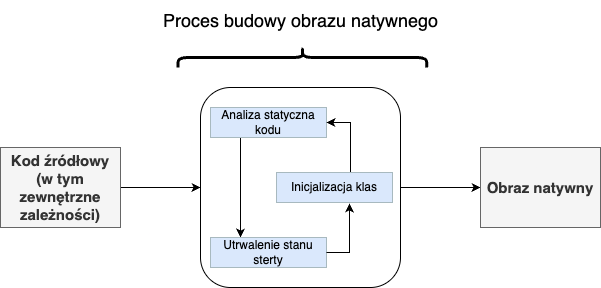
\includegraphics[width=0.95\textwidth]{charts/graalvm-build-process.drawio.png}
    \caption{Uproszczony proces budowy obrazu natywnego GraalVM [źródło:~opracowanie~własne]}
    \label{fig:graalvm_build_process}
\end{figure}

Kolejnym aspektem, który może negatywnie wpłynąć na rozwój oprogramowania przy użyciu GraalVM, jest czasochłonność procesu kompilacji.
Generowanie w pełni zoptymalizowanego obrazu natywnego jest operacją bardziej złożoną niż standardowa kompilacja kodu Javy do postaci bajtowej.
W praktyce oznacza to, że proces budowania artefaktu dla funkcji AWS Lambda może trwać odczuwalnie dłużej.
Może mieć to znaczący wpływ na rozwój oprogramowania, szczególnie w przypadku częstych iteracji i tworzenia nowych wersji funkcji.
Dłuższy czas kompilacji może także wpłynąć na ogólną efektywność procesów ciągłej integracji i ciągłego dostarczania (ang. CI/CD).

Jednym z sposobów poprawy doświadczeń programistów przy pracy z GraalVM, jest użycie odpowiednich frameworków.
Jednym z nich jest Quarkus \cite{9245290}, który został zaprojektowany z myślą o środowiskach chmurowych.
Kluczową cechą Quarkusa jest przeniesienie jak największej liczby operacji inicjalizacyjnych i konfiguracyjnych na etap budowania aplikacji.
Obejmuje to między innymi wstrzykiwanie zależności, przetwarzanie adnotacji oraz konfigurację rozszerzeń. 
Dzięki temu, w czasie budowania obrazu natywnego, Quarkus jest w stanie przeprowadzić szczegółową analizę aplikacji.
Poprzez użycie odpowiednich annotacji pozwala on na oznaczenie klas niezbędnych dla mechanizmów refleksji czy proxy \cite{quarkus-docs}.
Dzięki temu jest on w stanie automatycznie wygenerować niezbędne metadane dla klas.
Dane te następnie pozwalają na użycie wspomnianych mechanizmów w GraalVM.
Innymi, konkurencyjnymi do Quarkusa frameworkami, które oferują wsparcie dla obrazów natywnych są Helidon i Micronaut \cite{9245290}.
Ich popularność wskazuje na wysokie zainteresowanie takimi technologiami w społeczności programistów Java, dlatego jest to interesujący kierunek rozwoju dla funkcji AWS Lambda.

\section{Kotlin}\label{chapter:kotlin_multiplatform}

W ramach systematycznego przeglądu literatury (przedstawionego w Rozdziale \ref{chapter:przeglad_literatury}) zauważono, że aktualne badania skupiają się wyłącznie na języku Java.
Pomijają one jednak inne języki z ekosystemu Java, także oparte o maszynę wirtualną Java (ang. JVM).
Tymczasem na popularności zyskują alternatywne języki ekosystemu Javy.
Wśród nich na szczególną uwagę zasługuje Kotlin, rozwijany przez firmę JetBrains.
Jest on oficjalnie wspierany przez Google jako język programowania dla platformy Android, co wskazuje na jego solidne zastosowanie w tych systemach.
Coraz większe uznanie zyskuje także jako działający po stronie serwera. 
Dlatego język ten jest interesującym obszarem badań w kontekście AWS Lambda.
W tym rozdziale przedstawiony zostanie język programowania Kotlin, w tym jego zastosowanie w kontekście funkcji AWS Lambda.

Jednym z kluczowych czynników, które zwiększają popularność Kotlina, jest jego łatwa nauka przez programistów Javy.
Dodatkowo, istnieje możliwość łatwej intergracji kodu napisanego w Kotlinie z istniejącym oprogramowaniem Java \cite{kotlinlangKotlinDocs}.
Te cechy czynią go interesującym kandydatem do analizy w kontekście optymalizacji wydajności rozwiązań dla usługi AWS Lambda. 
Dla zespołów programistycznych może stanowić on wartościowe rozszerzenie dotychczasowych możliwości. 
Kotlin oferuje bowiem alternatywę lub uzupełnienie dla tradycyjnie stosowanej Javy.

Kwestia wydajności Kotlina w porównaniu do Javy jest przedmiotem dyskusji. 
Jednak badania dotyczą najczęściej ich zastosowań w kontekście aplikacji mobilnych.
Gajek i inni autorzy \cite{Gajek_Plechawska-Wójcik_2024} przeanalizowali wydajność obu języków, poprzez użycie gry mobilnej uruchomionej na systemie Android.
Wykazali oni, że w testowanym scenariuszu Java osiągnęła nieznacznie lepszą wydajność pod względem zużycia zasobów CPU i RAM.
Było to jednak zastosowanie mobilne, a same różnice nie były znaczne.
Należy jednak podkreślić, że warunki mobilne mogą być inne niż w systemach działających w usłudze AWS Lambda.
Sam język Kotlin posiada mechanizmy, które mogą pozytywnie wpłynąć na wydajność.

Funkcje inline (ang. inline functions) w Kotlinie mogą przyczynić się do redukcji narzutu wydajności podczas wywołań funkcji.
Mechanizm ten polega na wstawieniu kodu ciała funkcji bezpośrednio w miejsce jej wywołania \cite{kotlinlangKotlinDocs}.
Jest to wykonywane w momencie kompilacji, a programista może określić, które funkcje powinny być w ten sposób optymalizowane.
Eliminuje to koszt ich wywołania, co jest szczególnie przydatne w przypadku małych, często używanych funkcji.
Dodatkowo, język pozwala na przekazywanie funkcji jako parametrów, na przykład w kolekcjach i metodach jak filtrowanie.
W tych sytuacjach użycie funkcji inline może znacząco zmniejszyć liczbę operacji.
Pozytywny wpływ mechanizmu inline został przedstawiony przez Bergstrom i innych autorów \cite{DBLP:journals/corr/BergstromFRS13}, gdzie jego użycie zmniejszyło czas wykonywania programów nawet do 8\%.

Innym istotnym elementem Kotlina wspierającym wydajność są korutyny (ang. coroutines).
Mogą być one użyteczne zwłaszcza w kontekście operacji wejścia-wyjścia (I/O).
Systemy oparte o usługę AWS Lambda często integrowane są z zewnętrznymi serwisami (co zostało zauważone w ramach przeglądu literatury w Rozdziale \ref{chapter:przeglad_literatury}).
Wymaga to komunikacji opartej o operacje sieciowe.
Tradycyjne podejście oparte na wątkach może konsumować dużą ilość zasobów serwera i prowadzić do blokowania wykonania.
Korutyny pozwalają na pisanie asynchronicznego, nieblokującego kodu w sposób bardziej sekwencyjny i czytelny \cite{kotlinlangKotlinDocs}.
Na lepszą wydajność korutyn w porównaniu z tradycyjnymi wątkami wskazali Beronić i inni autorzy \cite{9803765}.

Implementacja mechanizmów poprawiających wydajność w języku programowania, pozwala następnie na ich użycie w bibliotekach, które są wykorzystywane przez programistów.
Język Kotlin oferuje ciekawy ekosystem bibliotek, przeznaczonych na przykład do tworzenia aplikacji działających po stronie serwera.
Są to biblioteki jak http4k czy ktor.
Ktor to framework zaprojektowany do budowy asynchronicznych aplikacji serwerowych i klienckich, rozwijany przez firmę JetBrains.
Jest on oparty w pełni o język Kotlin, a jego kluczową cechą jest natywne wsparcie dla korutyn.
Z kolei http4k kładzie nacisk na prostotę i minimalizm.
Architektura http4k opiera się na koncepcji funkcji jako podstawowych bloków aplikacji \cite{http4kCoreDocs}, co naturalnie współgra z modelem serverless i AWS Lambda.
Samo narzędzie rezyguje z mechanizmów refleksji \cite{http4kCoreDocs}, co może mieć pozytywny wpływ na wydajność.

Rosnące znaczenie Kotlin dostrzega także Amazon Web Service, które oferuje bibliotekę AWS SDK dla Kotlina \cite{awsSDKForKotlinDeveloperGuide}.
Jej celem jest zapewnienie programistom możliwości interakcji z usługami AWS w sposób naturalny dla tego języka.
SDK ten został zaprojektowany od podstaw z myślą o Kotlinie, co przejawia się między innymi w wykorzystaniu korutyn do obsługi operacji asynchronicznych.

Duży wpływ na wydajność funkcji AWS Lambda ma wybrany język programowania \cite{8605773}\cite{Cordingly2020704}.
Wynika to na przykład z różnych przypadków biznesowych i operacji, które muszą wykonywać.
Mimo to, często muszą one dzielić wspólny kod \cite{8116416}, co wskazuje na potrzebę wykorzystania mechanizmów, które to umożliwą.
Z tego powodu bardzo interesującą dla AWS Lambda i jej wydajności, może okazać się inicjatywa Kotlin Multiplatform.
KMP (Kotlin Multiplatform) to projekt, który powstał w szczególności dla aplikacji mobilnych.
Pozwala on na kompilację lub translację tego samego kodu Kotlin do użycia na różnych platformach.
Mogą to być na przykład Android, iOS, aplikacje desktopowe (JVM) lub webowe (JavaScript, Web Assembly) \cite{kotlinlangKotlinDocs}.
Oferuje to możliwość dzielenia kodu (np. logiki biznesowej) pomiędzy różnymi platformami, jednak przy możliwości zachowania natywnych komponentów widoku.

Mimo głównego przypadku użycia jakim są aplikacje klienckie, Kotlin Multiplatform może być obiecującym rozwiązaniem dla AWS Lambda.
Po pierwsze oferuje on możliwość translacji kodu Kotlin do JavaScript oraz kompilację do natywnych plików binarnych (opcje te zostaną przedstawione jako osobne metody w kolejnych rozdziałach).
Pozwala to na ominięcie różnych niedogodności wynikających z użycia maszyny wirtualnej Javy.
Jednak zachowane są przy tym zalety języka oraz wspiera to użycie już istniejących umiejętności programistów języków rodziny JVM.
Po drugie, kod w KMP może być dzielony pomiędzy platformami.
Umożliwia to bardzo elastyczny wybór środowiska uruchomieniowego AWS Lambda w ramach pojedynczego systemu.
Jednocześnie, część kodu może być współdzielona między wszystkie funkcje niezależnie od wybranej platformy.
Może to na przykład oznaczać, że klasy implementujące pewne struktury oraz zasady wynikające z reguł biznesowych, będą mogły być używane przez funkcje działające zarówno poprzez JavaScript, JVM, jak i natywne pliki binarne. 

Jednym z czynników, które mogą być modyfikowane już podczas działania usług AWS Lambda jest pamięć.
Jej rozmiar może być dostosowywany w zależności od wydajności monitorowanej funkcji.
Użycie Kotlin Multiplatform pozwala na rozszerzenie tej metody.
W zależności od obserwowanych parametrów (jak czas odpowiedzi lub opóźnienia zimnych startów) możliwe jest ponowne wykorzystanie tego samego kodu i budowa funkcji działającej na innej platformie.
Przykładowo, po wdrożeniu funkcji działającej z użyciem JVM, może pojawić się potrzeba redukcji czasu zimnych startów.
W takim wypadku Kotlin Multiplatform umożliwia translację kodu do JavaScript, który pozwoli na redukcję czasu inicjalizacji AWS Lambda.

Współdzielenie kodu pomiędzy platformami jest możliwe dzięki strukturze, którą oferuje Kotlin Multiplatform.
Została ona opisana przez firmę JetBrains w ramach dokumentacji KMP \cite{kotlinMultiplatformDev}.
Jej głównym elementem jest katalog ,,commonMain'', który jest współdzielony pomiędzy wszystkimi platformami.
Kompilator używa kodu współdzielonego jako dane wejściowe, aby w rezultacie utworzyć zestaw plików binarnych specyficznych dla danej platformy.
Mogą to być na przykład pliki .class dla maszyny wirtualnej Javy, czy natywne pliki wykonywalne (np. dla platformy Linux).

\begin{figure}[h]
    \centering
    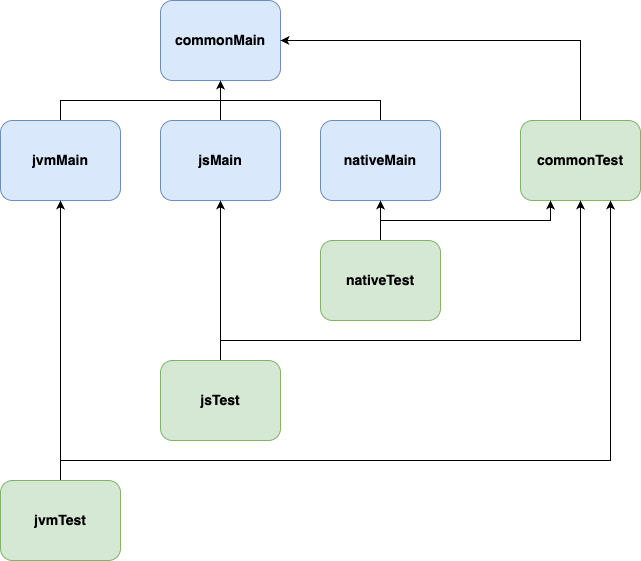
\includegraphics[width=0.95\textwidth]{charts/kmp-structure.drawio.png}
    \caption{Przykładowa struktura pojektu Kotlin Multiplatform [źródło:~opracowanie~własne]}
    \label{fig:kmp_project_structure}
\end{figure}

Następnie programista może utworzyć kolejne katalogi, które będą zawierać kod specyficzny dla docelowych platform.
Przykładowa struktura została przedstawiona na Rysunku \ref{fig:kmp_project_structure}, gdzie katalog commonMain jest wspóldzielony między JVM (jvmMain), JavaScript (jsMain) oraz platformy natywne (nativeMain).
Docelowe platformy (ang. targets) są deklarowane w konfiguracji Gradle \cite{kotlinMultiplatformDev}, a kod współdzielony jest przygotowywany wyłącznie dla nich.
Katalogi dla docelowych platform są wymagane, gdyż Kotlin nie zezwala na użycie specyficznych elementów danej platformy w katalogu współdzielonym.
Przykładem takiego elementu może być klasa ,,java.io.File'', która jest dostępna wyłącznie dla maszyny wirtualnej Javy.
Jej użycie w katalogu commonMain spowoduje błąd kompilacji.

Kotlin Multiplatform zawiera także integracje z testami oprogramowania.
Jest to szczególnie ważne dla tworzenia oprogramowania z wykorzystaniem AWS Lambda, gdzie testowanie może być skomplikowane (co było jednym z wniosków przeglądu literatury w Rozdziale \ref{chapter:przeglad_literatury}).
Testy dla kodu współdzielonego powinny być zapisane w katalogu ,,commonTest'', gdzie programista może użyć biblioteki kotlin.test \cite{kotlinMultiplatformDev}.
Następnie testy są uruchamiane dla każdej docelowej platformy.
Programista może także tworzyć przypadki testowe dla konkretnych platform, z użyciem technologii przez nie oferowanych.
Następuje tutaj analogiczne współdzielenie kodu jak dla katalogów ,,main'', co zostało także zawarte w Rysunku \ref{fig:kmp_project_structure}.

Specyficzne cechy Kotlina jak funkcjonalności języka, biblioteki czy projekt Kotlin Multiplatform mogą zapewnić znaczne wzrosty wydajności funkcji AWS Lambda.
Mimo, że Kotlin jest językiem wywodzącym się z Javy oferuje już możliwości, które mogą pozwolić na osiągnięcie niższych czasów odpowiedzi.
Dodatkowo, sposoby te nie zostały jeszcze przebadane. 
Dlatego Kotlin to obszar, który zasługuje na zawarcie go w badanich na temat wydajności AWS Lambda.

\section{Kotlin/JS}\label{chapter:kotlin_js}

\section{Kotlin/Native}\label{chapter:kotlin_native}

Bardzo skuteczną metodą optymalizacji wydajności może być rezygnacja z zarządzanych środowisk uruchomieniowych jak JVM.
Jedną z metod jest kompilacja do kodu natywnego, który uruchamiany jest bezpośrednio na systemie operacyjnym poza maszyną wirtualną.
Kotlin/Native oferuje zaawansową kompilację kodu Kotlin, który następnie może zostać uruchomiony w AWS Lambda z użyciem Amazon Linux.
W ramach rozdziału opisano sposób działania Kotlin/Native, jego możliwości i cechy, które mogą negatywnie wpłynąć na rozwój oprogramowania bezserwerowego.

Kluczowym elementami Kotlin/Native są kompilator oparty o LLVM oraz natywne implementacje bibliotek standardowych Kotlina \cite{kotlinlangKotlinDocs}.
Jak opisują Lattner i Adve \cite{1281665}, LLVM to framework kompilatora zaprojektowany do wspierania ciągłej i transparentnej analizy oraz transformacji programów.
Definiuje on wspólną, niskopoziomową reprezentację kodu w formie SSA (ang. Static Single Assignment) z systemem typów niezależnym od języka, co umożliwia implementację cech języków wysokiego poziomu. 
Głównym celem LLVM jest umożliwienie analizy i transformacji programu na różnych etapach jego życia, w tym w czasie kompilacji, linkowania, uruchomienia oraz w czasie bezczynności między uruchomieniami.
Jego użycie pozwala następnie na zbudowanie natywnych plików binarnych, które mogą zostać uruchomione bezpośrednio na docelowej platformie, dla której zostały skompilowane.
Wymaga to jednak dokładnego określenia systemu operacyjnego i architektury już w momencie kompilacji.

Kompilacja Kotlina do kodu natywnego otwiera przez KMP możliwość tworzenia samodzielnych programów wykonywalnych, które nie wymagają zewnętrznego środowiska uruchomieniowego.
Znajduje to zastosowanie w scenariuszach takich jak rozwój aplikacji mobilnych na platformę iOS, współdzielenie logiki biznesowej między różnymi platformami (np. Android i iOS) czy budowa narzędzi konsolowych.
Dlatego ważnym aspektem Kotlin/Native jest współdziałanie z istniejącym kodem natywnym.
Pozwala to na bezpośrednie wywoływanie funkcji z bibliotek napisanych w języku C, a na platformach firmy Apple również Objective-C \cite{kotlinlangKotlinDocs}.
Znacząco rozszerza to zakres dostępnych narzędzi i bibliotek, które mogą zostać użyte przez programistów.

Kotlin/Native oferuje wiele różnych platform docelowych, rozszerzając tym samym zakres zastosowań języka Kotlin.
Wśród wspieranych systemów docelowych znajdują się platformy Apple (takie jak macOS, iOS, watchOS, tvOS), Android, a także systemy z rodziny Windows oraz Linux \cite{kotlinlangKotlinDocs}.
Szczególnie istotnie dla usługi AWS Lambda są jednak platformy linuxowe.
Są to linuxX64 oraz linuxArm64, które pozwalają na uruchomienie kodu z użyciem odpowiednio architektur x86 oraz ARM.
Pozwala to następnie na ich bezpośrednie użycie w AWS Lambda, działającej bezpośrednio w systemie Amazon Linux.
Dzięki temu możliwa jest poprawa wydajności, szczególnie w aspekcie zimnych startów, które są znacznym wyzwaniem dla funkcji opartych o JVM.

Istotnym elementen funkcji bezserwerowych jest zarządzanie pamięcią, która wpływa bezpośrednio na koszty.
W przypadku Kotlin/Native, ewolucja modelu zarządzania pamięcią znacząco wpłynęła na jego użyteczność i możliwości optymalizacyjne.
Początkowa technologia ta opierała się na restrykcyjnym modelu z izolacją obiektów między wątkami \cite{kotlinlangKotlinDocs}.
Powodowało to skomplikowane zarządzanie stanem w operacjach współbieżnych.
Aktualnie, Kotlin/Native implementuje nowy menedżer pamięci.
Wprowadza on automatyczne zarządzanie pamięcią poprzez współbieżny, nieblokujący moduł zbierania śmieci (ang. garbage collector) \cite{kotlinlangKotlinDocs}.
Znacząco upraszcza to programowanie współbieżne, które teraz nie wymaga ręcznego zarządzania obiektami.
Mechanizm ten wprowadza intuicyjne współdzielenie stanu, które jest analogiczne do środowiska JVM, jednak bez konieczności kosztownej obsługi maszyny wirtualnej Java.

Mimo potencjalnych zysków w ramach wydajności, użycie Kotlin/Native może nieść utrudnienia w kontekście integracji z bibliotekami zewnętrznymi.
Język C nie jest oficjalnie wspierany jako język programowania AWS Lambda \cite{awsLambdaDeveloperGuide}, co wynika zapewne z jego niewielkiej popularności na tej platformie.
Współdziałanie z kodem natywnym w Kotlin/Native skupia się jednak na platformach klienckich, co nie musi być do końca użyteczne w zakresie AWS Lambda.
Amazon Web Services oferuje swoje SDK w języku C++, który nie jest jednak łatwo integrowalny z Kotlin/Native (w odróżnieniu od C i Objective-C).
Jest to ważny czynnik, który powinien być uwzględniony przez programistów projektujących aplikacje bezserwerowe.

% Plan
% 0. Wstęp

% 1. Jak to działa:
% - Opisać LLVM
% - Gdzie się głównie używa
% - Wspomnieć o interoperacyjności z C, Objective-C itp
% - Jakie platformy? (https://kotlinlang.org/docs/native-target-support.html#for-library-authors)

% 2. Zarządzanie pamięcią (https://kotlinlang.org/docs/native-memory-manager.html)

% 3. Wady - problem z dostępnością bibliotek
% - AWS SDK może poprzez C++ jednak może to wymagać większego nakładu pracy


\newpage

\pagestyle{customUnnumberedStyle}
\chapter{Wybrane metody optymalizacji}\label{chapter:wybrane_metody_optimalizacji}

% TODO: jakiś wstęp, typu jakich metod brakowało w przeglądzie. Podkreślić brak innych języków
\section{SnapStart}\label{chapter:snapstart}

Jednym z istotnych czynników wpływających na wydajność funkcji AWS Lambda implementowanych w ekosystemie Java jest zjawisko tzw. zimnego startu.
Wynika on z cyklu życia funkcji i etapu inicjalizacji (co zostało opisane w Rozdziale \ref{chapter:aws_lambda}).
W etap ten wchodzą procesy takie jak inicjalizacja maszyny wirtualnej Java czy uruchomienie statycznego kodu inicjującego \cite{awsLambdaDocs}.
W przypadku Javy zajmuje to więcej czasu niż dla innych języków (jak Python), co wydłuża zimne starty \cite{8605773}.
Znacząco oddziałuje to na wydajność funkcji, a może być szczególnie dotkliwe dla serwisów o niewielkiej aktywności.
W odpowiedzi na potrzebę minimalizacji tych negatywnych skutków Amazon Web Services wprowadziło mechanizm znany jako AWS Lambda SnapStart.
W ramach podrozdziału podjęto analizę tego rozwiązania w kontekście jego działania, zalet oraz ograniczeń. 

Mechanizm SnapStart istotnie modyfikuje tradycyjny cykl życia funkcji AWS Lambda.
Zasadnicza różnica polega na przeniesieniu kosztownego etapu inicjalizacji z momentu pierwszego wywołania funkcji na etap jej publikacji \cite{amazonSnapstartDeveloperGUide}.
Oznacza to, że inicjalizacja funkcji nie jest wykonywana w momencie zapytania użytkownika (co wywołuje zimny start), lecz w momencie wgrania nowej wersji funkcji (oraz kodu) przez programistę.
Inicjalizacja ta zawiera najdłuższe operacje dla rozwiązań Java jak utworzenie maszyny wirtualnej, załadowanie klas, czy wykonanie kodu inicjalizującego.
Następnie, tworzona jest zaszyfrowana ,,migawka'' (ang. snapshot) stanu pamięci i dysku w pełni gotowego środowiska wykonawczego.
Gdy funkcja jest następnie wywoływana po raz pierwszy, nie zachodzi już standardowy zimny start.
Zamiast tego środowisko jest odtwarzane z utworzonej migawki, co zostało przedstawione na Rysunku \ref{fig:aws_lambda_snapstart_process}.
Według dostawcy AWS metoda ta w optymalnych scenariuszach zmniejsza opóźnienie z kilku sekund do mniej niż sekundy \cite{amazonSnapstartDeveloperGUide}. 

\begin{figure}[h]
    \centering
    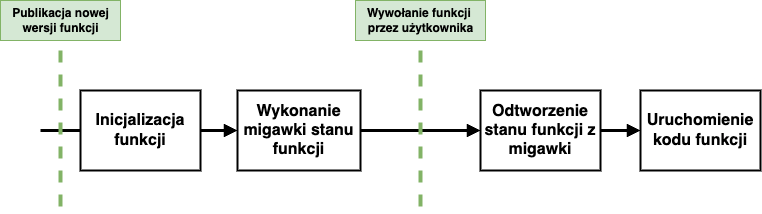
\includegraphics[width=0.95\textwidth]{charts/snapstart.png}
    \caption{Proces uruchomienia AWS Lambda z użyciem metody SnapStart [źródło:~opracowanie~własne]}
    \label{fig:aws_lambda_snapstart_process}
\end{figure}

Działanie tej metody jest technicznie możliwe dzięki użyciu środowiska wirtualizacji przez AWS Lambda.
Jak opisują Agache i inni autorzy \cite{246288} usługa Lambda do izolacji poszczególnych funkcji wykorzystuje dedykowane maszyny wirtualne typu microVM.
Są one zarządzane przez lekki monitor maszyn wirtualnych (ang. VMM) o nazwie Firecracker.
Posiada on cechy, które były kluczowe w minimalizacji problemu zimnego startu.
Po pierwsze, celowo rezygnuje on z emulacji zbędnych urządzeń (jak emulacja systemu BIOS czy rozbudowanych kontrolerów PCI) \cite{246288}.
Zmniejsza to złożoność i rozmiar stanu każdej maszyny wirtualnej. 
Dzięki temu wykonanie i odtworzenie migawki jest łatwiejsze.
Po drugie, Firecracker jest w pełni kontrolowany przez interfejs REST API \cite{246288}.
Umożliwia to precyzyjne zarządzanie całym cyklem życia każdej maszyny wirtualnej, włączając w to jej konfigurację, uruchomienie oraz zatrzymanie.
Pozwala to na określenie fazy inicjalizacji funkcji oraz wykonanie migawki w odpowiednim momencie.
Istotna jest również zapewniona przez Firecracker izolacja \cite{246288}, co gwarantuje bezpieczeństwo tworzenia i odtwarzania migawek.

Samo użycie metody SnapStart jest bardzo proste i nie wymaga od programisty dużego nakładu pracy.
Włączenie rozwiązania wymaga jedynie ustawienia odpowiedniej opcji podczas konfiguracji funkcji \cite{amazonSnapstartDeveloperGUide}.
Nie oznacza to jednak, że SnapStart jest odpowiedni dla wszystkich funkcji.
AWS podkreśla dwa typy aplikacji, które znacząco zyskają poprzez użycie SnapStart \cite{amazonSnapstartDeveloperGUide}.
Są nimi wrażliwe na opóźnienia interfejsy API i potoki przetwarzania danych.
Dodatkowo, metoda ta niesie za sobą pewne ograniczenia, które muszą zostać uwzględnione przed jej wdrożeniem.

Pierwszym aspektem jest kwestia unikalności stanu w funkcjach wykorzystujących SnapStart.
Jak analizują Brooker i inni autorzy \cite{brooker2021restoringuniquenessmicrovmsnapshots}, klonowanie migawek wprowadza fundamentalne wyzwanie związane z przywróceniem unikalności maszyn wirtualnych, co jest niezbędne do poprawnego generowania unikalnych identyfikatorów czy sekretów kryptograficznych.
Migawka zainicjowanego środowiska wykonywana jest jednorazowo, a następnie używana podczas wielu wywołań funkcji.
Może to stanowić duże zagrożenie dla programisty AWS Lambda, gdy potrzebuje on generować unikalne wartości jak identyfikatory (np. UUID) czy jednorazowe tokeny.
Narusza to znacznie poprawność logiki aplikacji oraz jej bezpieczeństwo.
Jedną z metod naprawy tego problemu jest generowanie wartości losowych wyłącznie w metodzie wywołującej funkcje (zamiast w bloku statycznym kodu) \cite{amazonSnapstartDeveloperGUide}.
Dodatkowo, ewentualne problemy z unikalnością funkcji SnapStart mogą zostać wykryte poprzez oprogramowanie SpotBugs \cite{SpotBugsProject}.
Narzędzie wykonuje statyczną analizę kodu, walidując go poprzez reguły zapewnione przez AWS.
Pozwala to programiście wykryć, a następnie naprawić fragmenty kodu powodujące problem z unikalnością.

Kolejnym istotnym wyzwaniem podczas rozwoju aplikacji z technologią SnapStart jest zarządzanie połączeniami sieciowymi \cite{amazonSnapstartDeveloperGUide}.
Połączenia nawiązane z zewnętrznymi usługami są standardową praktyką podczas tworzenia aplikacji AWS Lambda \cite{eismann2021reviewserverlessusecases}\cite{Ivanov_Petrova_2024}.
Problematyczne stają się jednak te połączenia sieciowe, które nawiązano podczas inicjalizacji funkcji. 
Ponieważ inicjalizacja odbywa się przed faktycznym przetworzeniem żądania użytkownika, upływający czas może sprawić, że w momencie odtworzenia funkcji połączenia te nie będą już aktywne.
Praktyką zalecaną przez AWS jest ponowne nawiązywanie lub dokładna walidacja istniejących połączeń \cite{amazonSnapstartDeveloperGUide}.
Powinno to być wykonane bezpośrednio w metodzie wywołującej funkcje lub z wykorzystaniem metody ,,afterRestore''.
Metoda ta jest wywoływana bezpośrednio po odtworzeniu migawki stanu funkcji.

Strategicznym czynnikiem usług bezserwerowych są koszty, zatem powinny być one uwzględnione także przed użyciem SnapStart.
Zgodnie z dokumentacją Amazon Web Services \cite{amazonSnapstartDeveloperGUide}, użycie SnapStart dla środowisk uruchomieniowych Java nie wiążą się z dodatkowymi kosztami.
Koszt wykonania funkcji z włączonym SnapStart nadal bazuje na standardowych rozliczeniach.
Składa się na niego liczba przetworzonych żądań oraz łączny czas trwania wykonań.

Podsumowując, mechanizm SnapStart stanowi prostą w aktywacji metodę redukcji czasu zimnych startów.
Sam mechanizm opiera się na wcześniejszym wykonaniu fazy inicjacji funkcji, a następnie wykonania migawki stanu.
W momencie wywołania funkcji stan ten może zostać odtworzony.
Znaczącą korzyścią metody jest brak dodatkowych kosztów.
Wiąże się ona jednak z istotnymi utrudnieniami (jak zarządzanie połączeniami sieciowymi i problem z unikalnością stanu).
Powinny być one uwzględnione przez programistę przed użyciem narzędzia.
\section{GraalVM}\label{chapter:graalvm}

Ważnym obszarem badań nad optymalizacją Javy i jej użycia w AWS Lambda, są technologie pozwalające na zmianę sposobu kompilacji i uruchamiana aplikacji.
Jedną z technologii, które zyskusje na popularności w tym zakresie, jest GraalVM.
Jest to możliwe m.in. dzięki użyciu kompilatora JIT (ang. Just-In-Time) w połączeniu z kompilacją AOT (ang. Ahead-Of-Time) \cite{8756917}.
GraalVM oferuje zaawansowaną architekturę pozwalającą na kompilację i uruchomienie aplikacji w postaci obrazów natywnych.
Stanowi to alternatywę dla klasycznej maszyny wirtualnej Javy, a dodatkowo skupia się na jej wydajności.
Poniższy podrozdział poświęcono analizie działania omawianego rozwiązania, jego zalet i słabych stron.

Kluczowym mechanizmem GraalVM jest kompilacja AOT (ang. Ahead-Of-Time) do postaci tzw. obrazów natywnych (ang. native images) \cite{8756917}.
Ma to bezpośredni wpływ na wydajność działania aplikacji.
W modelu tradycyjnym, kod bajtowy Java jest interpretowany i kompilowany dynamicznie przez maszynę wirtualną w trakcie działania aplikacji.
Podejście AOT przenosi znaczną część z tych operacji na etap budowania artefaktu. 
Istotnym elementem tego procesu jest agresywna, statyczna analiza kodu \cite{9245290}, w celu identyfikacji osiągalnych w trakcie działania części.
Pozwala to na odrzucenie nieużywanych fragmentów kodu (np. z używanych bibliotek), co pozwala na zmniejszenie wielkości obrazu natywnego.
Aspekt ten może być kluczowy w kontekście AWS Lambda, ze względu na wpływ wielkości artefaktu na wydajność \cite{8116416}.
Po analizie kodu, dokonywana jest inicjalizacja klas, a stan aplikacji, w tym częściowo zainicjalizowana sterta, jest utrwalany.
W celu lepszej optymalizacji, operacje te są powtarzane, co zostało przedstawione na Rysunku \ref{fig:graalvm_build_process}.

Jako wynik kompilacji powstaje samodzielny, zoptymalizowany plik binarny.
Nie wymaga on do uruchomienia pełnej maszyny wirtualnej Java, a jedynie minimalnego środowiska wykonawczego dostarczanego przez SubstrateVM, będącego częścią GraalVM \cite{8756917}.
Różnica ta ma fundamentalne znaczenie w kontekście wydajności AWS Lambda.
Eliminowana jest konieczność wykonywania czasochłonnych operacji typowych dla startu tradycyjnej maszyny wirtualnej Java, takich jak ładowanie klas czy jej inicjalizacja.
Wszystkie te zadania zostały już wykonane wcześniej, w procesie budowy obrazu natywnego.
Dzięki temu tworzona przez programistę funkcja AWS Lambda nie będzie operować w zarządzanym środowisku Java.
Zamiast tego, usługi muszą opierać się o niestandardowe środowiska wykonawcze, oferujące wyłącznie system operacyjny (Amazon Linux 2023 lub Amazon Linux 2) \cite{awsLambdaDeveloperGuide}.
Ich użycie pozwala także na realizację drugiej zalety GraalVM, czyli redukcji zapotrzebowania na pamięć operacyjną \cite{9245290}.

Pomimo pozytywnego wpływu na wydajność, zastosowanie kompilacji AOT w GraalVM wiąże się także z ograniczeniami.
Jednym z nich jest obsługa dynamicznych cech Javy, takich jak refleksja (ang. reflection), dynamiczne proxy, serializacja czy natywny interfejs Java (JNI)
Wynika to z faktu użycia agresywnej statycznej analizy kodu.
Napotyka ona trudności w przewidzeniu wszystkich dynamicznie ładowanych klas, pól i metod, które nie są jawnie osiągalne w kodzie źródłowym.
Problem ten wymaga użycia dodatkowych mechanizmów GraalVM \cite{graalvm-reflection-jdk21}.
Polegają one na przygotowaniu dodatkowych metadanych dla klas, co wymaga jednak dodatkowej obsługi.

\begin{figure}
    \centering
    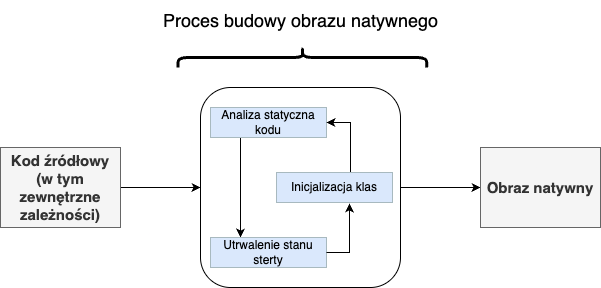
\includegraphics[width=0.95\textwidth]{charts/graalvm-build-process.drawio.png}
    \caption{Uproszczony proces budowy obrazu natywnego GraalVM [źródło:~opracowanie~własne]}
    \label{fig:graalvm_build_process}
\end{figure}

Kolejnym aspektem, który może negatywnie wpłynąć na rozwój oprogramowania przy użyciu GraalVM, jest czasochłonność procesu kompilacji.
Generowanie w pełni zoptymalizowanego obrazu natywnego jest operacją bardziej złożoną niż standardowa kompilacja kodu Javy do postaci bajtowej.
W praktyce oznacza to, że proces budowania artefaktu dla funkcji AWS Lambda może trwać odczuwalnie dłużej.
Może mieć to znaczący wpływ na rozwój oprogramowania, szczególnie w przypadku częstych iteracji i tworzenia nowych wersji funkcji.
Dłuższy czas kompilacji może także wpłynąć na ogólną efektywność procesów ciągłej integracji i ciągłego dostarczania (ang. CI/CD).

Jednym z sposobów poprawy doświadczeń programistów przy pracy z GraalVM, jest użycie odpowiednich frameworków.
Jednym z nich jest Quarkus \cite{9245290}, który został zaprojektowany z myślą o środowiskach chmurowych.
Kluczową cechą Quarkusa jest przeniesienie jak największej liczby operacji inicjalizacyjnych i konfiguracyjnych na etap budowania aplikacji.
Obejmuje to między innymi wstrzykiwanie zależności, przetwarzanie adnotacji oraz konfigurację rozszerzeń. 
Dzięki temu, w czasie budowania obrazu natywnego, Quarkus jest w stanie przeprowadzić szczegółową analizę aplikacji.
Poprzez użycie odpowiednich annotacji pozwala on na oznaczenie klas niezbędnych dla mechanizmów refleksji czy proxy \cite{quarkus-docs}.
Dzięki temu jest on w stanie automatycznie wygenerować niezbędne metadane dla klas.
Dane te następnie pozwalają na użycie wspomnianych mechanizmów w GraalVM.
Innymi, konkurencyjnymi do Quarkusa frameworkami, które oferują wsparcie dla obrazów natywnych są Helidon i Micronaut \cite{9245290}.
Ich popularność wskazuje na wysokie zainteresowanie takimi technologiami w społeczności programistów Java, dlatego jest to interesujący kierunek rozwoju dla funkcji AWS Lambda.

\section{Kotlin}\label{chapter:kotlin_multiplatform}

W ramach systematycznego przeglądu literatury (przedstawionego w Rozdziale \ref{chapter:przeglad_literatury}) zauważono, że aktualne badania skupiają się wyłącznie na języku Java.
Pomijają one jednak inne języki z ekosystemu Java, także oparte o maszynę wirtualną Java (ang. JVM).
Tymczasem na popularności zyskują alternatywne języki ekosystemu Javy.
Wśród nich na szczególną uwagę zasługuje Kotlin, rozwijany przez firmę JetBrains.
Jest on oficjalnie wspierany przez Google jako język programowania dla platformy Android, co wskazuje na jego solidne zastosowanie w tych systemach.
Coraz większe uznanie zyskuje także jako działający po stronie serwera. 
Dlatego język ten jest interesującym obszarem badań w kontekście AWS Lambda.
W tym rozdziale przedstawiony zostanie język programowania Kotlin, w tym jego zastosowanie w kontekście funkcji AWS Lambda.

Jednym z kluczowych czynników, które zwiększają popularność Kotlina, jest jego łatwa nauka przez programistów Javy.
Dodatkowo, istnieje możliwość łatwej intergracji kodu napisanego w Kotlinie z istniejącym oprogramowaniem Java \cite{kotlinlangKotlinDocs}.
Te cechy czynią go interesującym kandydatem do analizy w kontekście optymalizacji wydajności rozwiązań dla usługi AWS Lambda. 
Dla zespołów programistycznych może stanowić on wartościowe rozszerzenie dotychczasowych możliwości. 
Kotlin oferuje bowiem alternatywę lub uzupełnienie dla tradycyjnie stosowanej Javy.

Kwestia wydajności Kotlina w porównaniu do Javy jest przedmiotem dyskusji. 
Jednak badania dotyczą najczęściej ich zastosowań w kontekście aplikacji mobilnych.
Gajek i inni autorzy \cite{Gajek_Plechawska-Wójcik_2024} przeanalizowali wydajność obu języków, poprzez użycie gry mobilnej uruchomionej na systemie Android.
Wykazali oni, że w testowanym scenariuszu Java osiągnęła nieznacznie lepszą wydajność pod względem zużycia zasobów CPU i RAM.
Było to jednak zastosowanie mobilne, a same różnice nie były znaczne.
Należy jednak podkreślić, że warunki mobilne mogą być inne niż w systemach działających w usłudze AWS Lambda.
Sam język Kotlin posiada mechanizmy, które mogą pozytywnie wpłynąć na wydajność.

Funkcje inline (ang. inline functions) w Kotlinie mogą przyczynić się do redukcji narzutu wydajności podczas wywołań funkcji.
Mechanizm ten polega na wstawieniu kodu ciała funkcji bezpośrednio w miejsce jej wywołania \cite{kotlinlangKotlinDocs}.
Jest to wykonywane w momencie kompilacji, a programista może określić, które funkcje powinny być w ten sposób optymalizowane.
Eliminuje to koszt ich wywołania, co jest szczególnie przydatne w przypadku małych, często używanych funkcji.
Dodatkowo, język pozwala na przekazywanie funkcji jako parametrów, na przykład w kolekcjach i metodach jak filtrowanie.
W tych sytuacjach użycie funkcji inline może znacząco zmniejszyć liczbę operacji.
Pozytywny wpływ mechanizmu inline został przedstawiony przez Bergstrom i innych autorów \cite{DBLP:journals/corr/BergstromFRS13}, gdzie jego użycie zmniejszyło czas wykonywania programów nawet do 8\%.

Innym istotnym elementem Kotlina wspierającym wydajność są korutyny (ang. coroutines).
Mogą być one użyteczne zwłaszcza w kontekście operacji wejścia-wyjścia (I/O).
Systemy oparte o usługę AWS Lambda często integrowane są z zewnętrznymi serwisami (co zostało zauważone w ramach przeglądu literatury w Rozdziale \ref{chapter:przeglad_literatury}).
Wymaga to komunikacji opartej o operacje sieciowe.
Tradycyjne podejście oparte na wątkach może konsumować dużą ilość zasobów serwera i prowadzić do blokowania wykonania.
Korutyny pozwalają na pisanie asynchronicznego, nieblokującego kodu w sposób bardziej sekwencyjny i czytelny \cite{kotlinlangKotlinDocs}.
Na lepszą wydajność korutyn w porównaniu z tradycyjnymi wątkami wskazali Beronić i inni autorzy \cite{9803765}.

Implementacja mechanizmów poprawiających wydajność w języku programowania, pozwala następnie na ich użycie w bibliotekach, które są wykorzystywane przez programistów.
Język Kotlin oferuje ciekawy ekosystem bibliotek, przeznaczonych na przykład do tworzenia aplikacji działających po stronie serwera.
Są to biblioteki jak http4k czy ktor.
Ktor to framework zaprojektowany do budowy asynchronicznych aplikacji serwerowych i klienckich, rozwijany przez firmę JetBrains.
Jest on oparty w pełni o język Kotlin, a jego kluczową cechą jest natywne wsparcie dla korutyn.
Z kolei http4k kładzie nacisk na prostotę i minimalizm.
Architektura http4k opiera się na koncepcji funkcji jako podstawowych bloków aplikacji \cite{http4kCoreDocs}, co naturalnie współgra z modelem serverless i AWS Lambda.
Samo narzędzie rezyguje z mechanizmów refleksji \cite{http4kCoreDocs}, co może mieć pozytywny wpływ na wydajność.

Rosnące znaczenie Kotlin dostrzega także Amazon Web Service, które oferuje bibliotekę AWS SDK dla Kotlina \cite{awsSDKForKotlinDeveloperGuide}.
Jej celem jest zapewnienie programistom możliwości interakcji z usługami AWS w sposób naturalny dla tego języka.
SDK ten został zaprojektowany od podstaw z myślą o Kotlinie, co przejawia się między innymi w wykorzystaniu korutyn do obsługi operacji asynchronicznych.

Duży wpływ na wydajność funkcji AWS Lambda ma wybrany język programowania \cite{8605773}\cite{Cordingly2020704}.
Wynika to na przykład z różnych przypadków biznesowych i operacji, które muszą wykonywać.
Mimo to, często muszą one dzielić wspólny kod \cite{8116416}, co wskazuje na potrzebę wykorzystania mechanizmów, które to umożliwą.
Z tego powodu bardzo interesującą dla AWS Lambda i jej wydajności, może okazać się inicjatywa Kotlin Multiplatform.
KMP (Kotlin Multiplatform) to projekt, który powstał w szczególności dla aplikacji mobilnych.
Pozwala on na kompilację lub translację tego samego kodu Kotlin do użycia na różnych platformach.
Mogą to być na przykład Android, iOS, aplikacje desktopowe (JVM) lub webowe (JavaScript, Web Assembly) \cite{kotlinlangKotlinDocs}.
Oferuje to możliwość dzielenia kodu (np. logiki biznesowej) pomiędzy różnymi platformami, jednak przy możliwości zachowania natywnych komponentów widoku.

Mimo głównego przypadku użycia jakim są aplikacje klienckie, Kotlin Multiplatform może być obiecującym rozwiązaniem dla AWS Lambda.
Po pierwsze oferuje on możliwość translacji kodu Kotlin do JavaScript oraz kompilację do natywnych plików binarnych (opcje te zostaną przedstawione jako osobne metody w kolejnych rozdziałach).
Pozwala to na ominięcie różnych niedogodności wynikających z użycia maszyny wirtualnej Javy.
Jednak zachowane są przy tym zalety języka oraz wspiera to użycie już istniejących umiejętności programistów języków rodziny JVM.
Po drugie, kod w KMP może być dzielony pomiędzy platformami.
Umożliwia to bardzo elastyczny wybór środowiska uruchomieniowego AWS Lambda w ramach pojedynczego systemu.
Jednocześnie, część kodu może być współdzielona między wszystkie funkcje niezależnie od wybranej platformy.
Może to na przykład oznaczać, że klasy implementujące pewne struktury oraz zasady wynikające z reguł biznesowych, będą mogły być używane przez funkcje działające zarówno poprzez JavaScript, JVM, jak i natywne pliki binarne. 

Jednym z czynników, które mogą być modyfikowane już podczas działania usług AWS Lambda jest pamięć.
Jej rozmiar może być dostosowywany w zależności od wydajności monitorowanej funkcji.
Użycie Kotlin Multiplatform pozwala na rozszerzenie tej metody.
W zależności od obserwowanych parametrów (jak czas odpowiedzi lub opóźnienia zimnych startów) możliwe jest ponowne wykorzystanie tego samego kodu i budowa funkcji działającej na innej platformie.
Przykładowo, po wdrożeniu funkcji działającej z użyciem JVM, może pojawić się potrzeba redukcji czasu zimnych startów.
W takim wypadku Kotlin Multiplatform umożliwia translację kodu do JavaScript, który pozwoli na redukcję czasu inicjalizacji AWS Lambda.

Współdzielenie kodu pomiędzy platformami jest możliwe dzięki strukturze, którą oferuje Kotlin Multiplatform.
Została ona opisana przez firmę JetBrains w ramach dokumentacji KMP \cite{kotlinMultiplatformDev}.
Jej głównym elementem jest katalog ,,commonMain'', który jest współdzielony pomiędzy wszystkimi platformami.
Kompilator używa kodu współdzielonego jako dane wejściowe, aby w rezultacie utworzyć zestaw plików binarnych specyficznych dla danej platformy.
Mogą to być na przykład pliki .class dla maszyny wirtualnej Javy, czy natywne pliki wykonywalne (np. dla platformy Linux).

\begin{figure}[h]
    \centering
    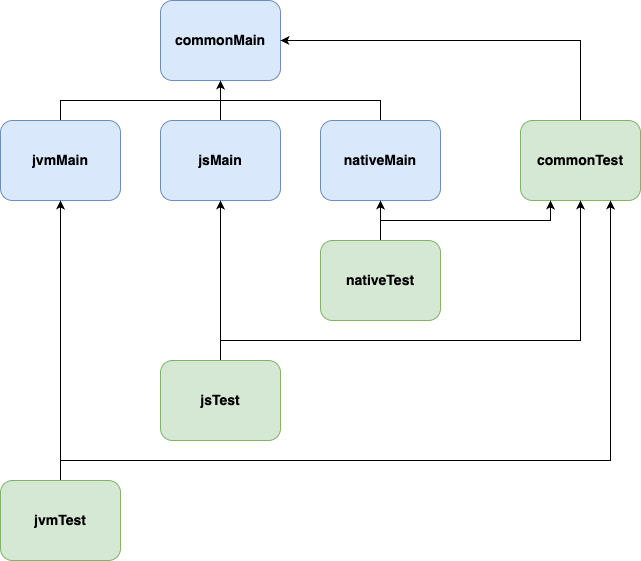
\includegraphics[width=0.95\textwidth]{charts/kmp-structure.drawio.png}
    \caption{Przykładowa struktura pojektu Kotlin Multiplatform [źródło:~opracowanie~własne]}
    \label{fig:kmp_project_structure}
\end{figure}

Następnie programista może utworzyć kolejne katalogi, które będą zawierać kod specyficzny dla docelowych platform.
Przykładowa struktura została przedstawiona na Rysunku \ref{fig:kmp_project_structure}, gdzie katalog commonMain jest wspóldzielony między JVM (jvmMain), JavaScript (jsMain) oraz platformy natywne (nativeMain).
Docelowe platformy (ang. targets) są deklarowane w konfiguracji Gradle \cite{kotlinMultiplatformDev}, a kod współdzielony jest przygotowywany wyłącznie dla nich.
Katalogi dla docelowych platform są wymagane, gdyż Kotlin nie zezwala na użycie specyficznych elementów danej platformy w katalogu współdzielonym.
Przykładem takiego elementu może być klasa ,,java.io.File'', która jest dostępna wyłącznie dla maszyny wirtualnej Javy.
Jej użycie w katalogu commonMain spowoduje błąd kompilacji.

Kotlin Multiplatform zawiera także integracje z testami oprogramowania.
Jest to szczególnie ważne dla tworzenia oprogramowania z wykorzystaniem AWS Lambda, gdzie testowanie może być skomplikowane (co było jednym z wniosków przeglądu literatury w Rozdziale \ref{chapter:przeglad_literatury}).
Testy dla kodu współdzielonego powinny być zapisane w katalogu ,,commonTest'', gdzie programista może użyć biblioteki kotlin.test \cite{kotlinMultiplatformDev}.
Następnie testy są uruchamiane dla każdej docelowej platformy.
Programista może także tworzyć przypadki testowe dla konkretnych platform, z użyciem technologii przez nie oferowanych.
Następuje tutaj analogiczne współdzielenie kodu jak dla katalogów ,,main'', co zostało także zawarte w Rysunku \ref{fig:kmp_project_structure}.

Specyficzne cechy Kotlina jak funkcjonalności języka, biblioteki czy projekt Kotlin Multiplatform mogą zapewnić znaczne wzrosty wydajności funkcji AWS Lambda.
Mimo, że Kotlin jest językiem wywodzącym się z Javy oferuje już możliwości, które mogą pozwolić na osiągnięcie niższych czasów odpowiedzi.
Dodatkowo, sposoby te nie zostały jeszcze przebadane. 
Dlatego Kotlin to obszar, który zasługuje na zawarcie go w badanich na temat wydajności AWS Lambda.

\section{Kotlin/JS}\label{chapter:kotlin_js}

\section{Kotlin/Native}\label{chapter:kotlin_native}

Bardzo skuteczną metodą optymalizacji wydajności może być rezygnacja z zarządzanych środowisk uruchomieniowych jak JVM.
Jedną z metod jest kompilacja do kodu natywnego, który uruchamiany jest bezpośrednio na systemie operacyjnym poza maszyną wirtualną.
Kotlin/Native oferuje zaawansową kompilację kodu Kotlin, który następnie może zostać uruchomiony w AWS Lambda z użyciem Amazon Linux.
W ramach rozdziału opisano sposób działania Kotlin/Native, jego możliwości i cechy, które mogą negatywnie wpłynąć na rozwój oprogramowania bezserwerowego.

Kluczowym elementami Kotlin/Native są kompilator oparty o LLVM oraz natywne implementacje bibliotek standardowych Kotlina \cite{kotlinlangKotlinDocs}.
Jak opisują Lattner i Adve \cite{1281665}, LLVM to framework kompilatora zaprojektowany do wspierania ciągłej i transparentnej analizy oraz transformacji programów.
Definiuje on wspólną, niskopoziomową reprezentację kodu w formie SSA (ang. Static Single Assignment) z systemem typów niezależnym od języka, co umożliwia implementację cech języków wysokiego poziomu. 
Głównym celem LLVM jest umożliwienie analizy i transformacji programu na różnych etapach jego życia, w tym w czasie kompilacji, linkowania, uruchomienia oraz w czasie bezczynności między uruchomieniami.
Jego użycie pozwala następnie na zbudowanie natywnych plików binarnych, które mogą zostać uruchomione bezpośrednio na docelowej platformie, dla której zostały skompilowane.
Wymaga to jednak dokładnego określenia systemu operacyjnego i architektury już w momencie kompilacji.

Kompilacja Kotlina do kodu natywnego otwiera przez KMP możliwość tworzenia samodzielnych programów wykonywalnych, które nie wymagają zewnętrznego środowiska uruchomieniowego.
Znajduje to zastosowanie w scenariuszach takich jak rozwój aplikacji mobilnych na platformę iOS, współdzielenie logiki biznesowej między różnymi platformami (np. Android i iOS) czy budowa narzędzi konsolowych.
Dlatego ważnym aspektem Kotlin/Native jest współdziałanie z istniejącym kodem natywnym.
Pozwala to na bezpośrednie wywoływanie funkcji z bibliotek napisanych w języku C, a na platformach firmy Apple również Objective-C \cite{kotlinlangKotlinDocs}.
Znacząco rozszerza to zakres dostępnych narzędzi i bibliotek, które mogą zostać użyte przez programistów.

Kotlin/Native oferuje wiele różnych platform docelowych, rozszerzając tym samym zakres zastosowań języka Kotlin.
Wśród wspieranych systemów docelowych znajdują się platformy Apple (takie jak macOS, iOS, watchOS, tvOS), Android, a także systemy z rodziny Windows oraz Linux \cite{kotlinlangKotlinDocs}.
Szczególnie istotnie dla usługi AWS Lambda są jednak platformy linuxowe.
Są to linuxX64 oraz linuxArm64, które pozwalają na uruchomienie kodu z użyciem odpowiednio architektur x86 oraz ARM.
Pozwala to następnie na ich bezpośrednie użycie w AWS Lambda, działającej bezpośrednio w systemie Amazon Linux.
Dzięki temu możliwa jest poprawa wydajności, szczególnie w aspekcie zimnych startów, które są znacznym wyzwaniem dla funkcji opartych o JVM.

Istotnym elementen funkcji bezserwerowych jest zarządzanie pamięcią, która wpływa bezpośrednio na koszty.
W przypadku Kotlin/Native, ewolucja modelu zarządzania pamięcią znacząco wpłynęła na jego użyteczność i możliwości optymalizacyjne.
Początkowa technologia ta opierała się na restrykcyjnym modelu z izolacją obiektów między wątkami \cite{kotlinlangKotlinDocs}.
Powodowało to skomplikowane zarządzanie stanem w operacjach współbieżnych.
Aktualnie, Kotlin/Native implementuje nowy menedżer pamięci.
Wprowadza on automatyczne zarządzanie pamięcią poprzez współbieżny, nieblokujący moduł zbierania śmieci (ang. garbage collector) \cite{kotlinlangKotlinDocs}.
Znacząco upraszcza to programowanie współbieżne, które teraz nie wymaga ręcznego zarządzania obiektami.
Mechanizm ten wprowadza intuicyjne współdzielenie stanu, które jest analogiczne do środowiska JVM, jednak bez konieczności kosztownej obsługi maszyny wirtualnej Java.

Mimo potencjalnych zysków w ramach wydajności, użycie Kotlin/Native może nieść utrudnienia w kontekście integracji z bibliotekami zewnętrznymi.
Język C nie jest oficjalnie wspierany jako język programowania AWS Lambda \cite{awsLambdaDeveloperGuide}, co wynika zapewne z jego niewielkiej popularności na tej platformie.
Współdziałanie z kodem natywnym w Kotlin/Native skupia się jednak na platformach klienckich, co nie musi być do końca użyteczne w zakresie AWS Lambda.
Amazon Web Services oferuje swoje SDK w języku C++, który nie jest jednak łatwo integrowalny z Kotlin/Native (w odróżnieniu od C i Objective-C).
Jest to ważny czynnik, który powinien być uwzględniony przez programistów projektujących aplikacje bezserwerowe.

% Plan
% 0. Wstęp

% 1. Jak to działa:
% - Opisać LLVM
% - Gdzie się głównie używa
% - Wspomnieć o interoperacyjności z C, Objective-C itp
% - Jakie platformy? (https://kotlinlang.org/docs/native-target-support.html#for-library-authors)

% 2. Zarządzanie pamięcią (https://kotlinlang.org/docs/native-memory-manager.html)

% 3. Wady - problem z dostępnością bibliotek
% - AWS SDK może poprzez C++ jednak może to wymagać większego nakładu pracy


\newpage

% Redefine plain for 1st bibliography page style
\resetformatting
% Please read :
%https://www.overleaf.com/learn/latex/Bibliography_management_with_bibtex
% \pagestyle{bibliographyStyle}
% \defbibfilter{bibliographyPapers}{
%   type=article or
%   type=inproceedings or
%   type=conference or
%   type=mastersthesis
% }
% \addcontentsline{toc}{chapter}{Bibliografia}  
% \printbibliography[filter=bibliographyPapers,title={Bibliografia}]
% \newpage

% \pagestyle{onlineSourcesStyle}
% \defbibfilter{onlinePapers}{
%   type=online or
%   type=misc or
%   type=manual
% }
% \addcontentsline{toc}{chapter}{Źródła internetowe}  
% \printbibliography[filter=onlinePapers,title={Źródła internetowe}]

\pagestyle{bibliographyStyle}
\addcontentsline{toc}{chapter}{Bibliografia}  
\printbibliography[title={Bibliografia}]
\newpage

% Add list of figures and tables
\pagestyle{custom}
\newpage
\pagestyle{ListofFiguresStyle}
\addcontentsline{toc}{chapter}{Spis rysunków}  
\listoffigures
\newpage
\pagestyle{ListofTablesStyle}
\addcontentsline{toc}{chapter}{Spis tabel}  
\listoftables

% % Redefine plain for 1st bibliography page style
% \resetformatting
% % Please read :
% %https://www.overleaf.com/learn/latex/Bibliography_management_with_bibtex
% \pagestyle{bibliographyStyle}
% \bibliographystyle{abbrv}
% \bibliography{sources/bibliography}

% %https://www.overleaf.com/learn/latex/Bibliography_management_with_bibtex
% % \pagestyle{bibliographyStyle}
% % \bibliographystyle{abbrv}
% % % zmienić tytuł
% % \bibliography{sources/internet_sources}

% % Add list of figures and tables
% \pagestyle{custom}
% \newpage
% \pagestyle{ListofFiguresStyle}
% \listoffigures
% \newpage
% \pagestyle{ListofTablesStyle}
% \listoftables

\end{document}